\documentclass[8 pt]{beamer}
\usepackage[utf8]{inputenc}
\usepackage{amsmath}
\usepackage{multirow}
\usepackage{cancel}
\usepackage{multicol}
\usepackage[document]{ragged2e}
\usepackage{hyperref}
\usepackage{xcolor}
\usepackage{color}
\usepackage{bm}
\usepackage{mathtools}
\definecolor{mygray}{gray}{0.7}
\renewcommand*{\arraystretch}{1.5}

\usetheme{EastLansing}
\setbeamertemplate{headline}{} %Remove section title
%\usetheme{Pittsburgh}
%\usetheme[height=30pt]{Rochester}
%\usecolortheme{lily}
%\usecolortheme{spruce}

\newcommand{\backupbegin}{
   \newcounter{finalframe}
   \setcounter{finalframe}{\value{framenumber}}
}
\newcommand{\backupend}{
   \setcounter{framenumber}{\value{finalframe}}
}

% -- East Lansing --
\definecolor{mydarkgreen}{RGB}{0,81,40}
\definecolor{mymediumgreen}{RGB}{153, 193, 173}
\definecolor{mylightgreen}{RGB}{229, 239, 234}
\definecolor{mycolor}{RGB}{0,81,40}

\setbeamertemplate{blocks}[rounded][shadow=false]
\setbeamercolor{structure}{fg=mydarkgreen}
\setbeamercolor*{block title}{fg=mydarkgreen, bg=mymediumgreen}
\setbeamercolor*{block body}{fg=black, bg=mylightgreen}

% -- Pittsburgh
%\definecolor{mycolor}{RGB}{51,51,180} %Dark blue
%\definecolor{mycolor}{RGB}{192,57,43} %Dark red
%\definecolor{mycolor}{RGB}{0,81,40} %Dark green

%\setbeamercolor*{title}{use=structure,fg=mycolor,bg=mycolor!12}
%\setbeamertemplate{title page}[default][colsep=-4bp,rounded=true,shadow=false]

%\setbeamertemplate{frametitle}
%{
%	\begin{center}\color{mycolor}\textbf{\Large\insertframetitle}\end{center} \vspace{-5pt}
%}

%\setbeamercolor{structure}{fg=mycolor}
%\setbeamercolor{itemize item}{fg=black}

\setbeamertemplate{blocks}[rounded][shadow=false]
\setbeamercolor*{block title}{fg=mycolor, bg=mycolor!12}
\setbeamercolor*{block body}{fg=black, bg=mycolor!12}

\setbeamercolor*{block title example}{fg=mycolor, bg=mycolor!4}
\setbeamercolor*{block body example}{fg=mycolor, bg=mycolor!12}
\setbeamersize{text margin left=6mm,text margin right=6mm} 
  
%\addtobeamertemplate{navigation symbols}{}{%
%    \usebeamerfont{footline}%
%   \usebeamercolor[fg]{footline}%
%   \hspace{1em}%
%    \insertframenumber/\inserttotalframenumber
%}

\title{Statistical approach to muography}
\date{July 17th 2020}
\author{C\'{e}dric Prie\"els}

 \begin{document}


\begin{frame}
\vspace{-15pt} 
\title{Development of a statistical analysis framework \\ in the context of Muography applied to the industry}
\author{C\'{e}dric Prie\"els \\ \vspace{10pt} \textbf{Director} - Pablo Mart\'inez Ru\'iz del \'Arbol \newline \textbf{Co-director} - Carlos D\'iez \\ \vspace{20pt} 
\includegraphics[width= 0.15\textwidth]{figs/image_UC.png} \hspace{10pt} 
\includegraphics[width= 0.16\textwidth]{figs/muonSystems.png} \newline \vspace{20pt} Universidad de Cantabria \newline Muon systems \newline  \begin{center} \large{\textbf{July 17th 2020}} \end{center}}

\date{}
\vspace{15pt}
\maketitle

\centering
  
\end{frame}


\begin{frame}{Table of contents}

	\begin{itemize}
		\item Introduction
		\begin{itemize}
			\item Muons, cosmic rays and and muography
			\item Experimental setup
		\end{itemize} \vfill
		\item Statistical basis of the algorithm
		\begin{itemize}
			\item Probability density functions
			\item Kernel density estimation
			\item Monte-Carlo simulations
			\item Likelihood minimization
		\end{itemize} \vfill
		\item Algorithm implementation
		\begin{itemize}
			\item PipeReconstructor, Generator, Plotter
		\end{itemize} \vfill
		\item Results obtained
		\begin{itemize}
			\item Generator validation
			\item Pipes geometries
			\item Likelihood curves
		\end{itemize} \vfill
		\item Conclusions \vfill
	\end{itemize}

\end{frame}






%Introduction
\begin{frame}{}
	\centering
	\huge{\textbf{\color{mycolor} Section I}} \newline
	\LARGE{\textbf{\color{mycolor} General introduction \color{black}}} \vfill
	
	\LARGE{\textbf{\color{black} \color{black}}}\newline \vspace{10pt} \Large{Develop a new framework allowing us to study the results from a muography experiment to characterize the inner properties of physical objects using data science and advanced statistical models.} \vfill
\end{frame}















%Theoretical introduction
\begin{frame}{Particle physics and muons}

\begin{minipage}[c]{.54\textwidth}
The Standard Model \textbf{describes the fundamental particles} existing and their interactions:
\begin{itemize}
	\justifying
	\item Introduced in the 1970s and still considered to be valid, but probably incomplete
	\item Simple in concept but extremely precise
	\item Lots of successful predictions made over the years, such as the existence of the top quark and the Higgs boson
\end{itemize}
\end{minipage} \hfill
\begin{minipage}[c]{.42\textwidth}
	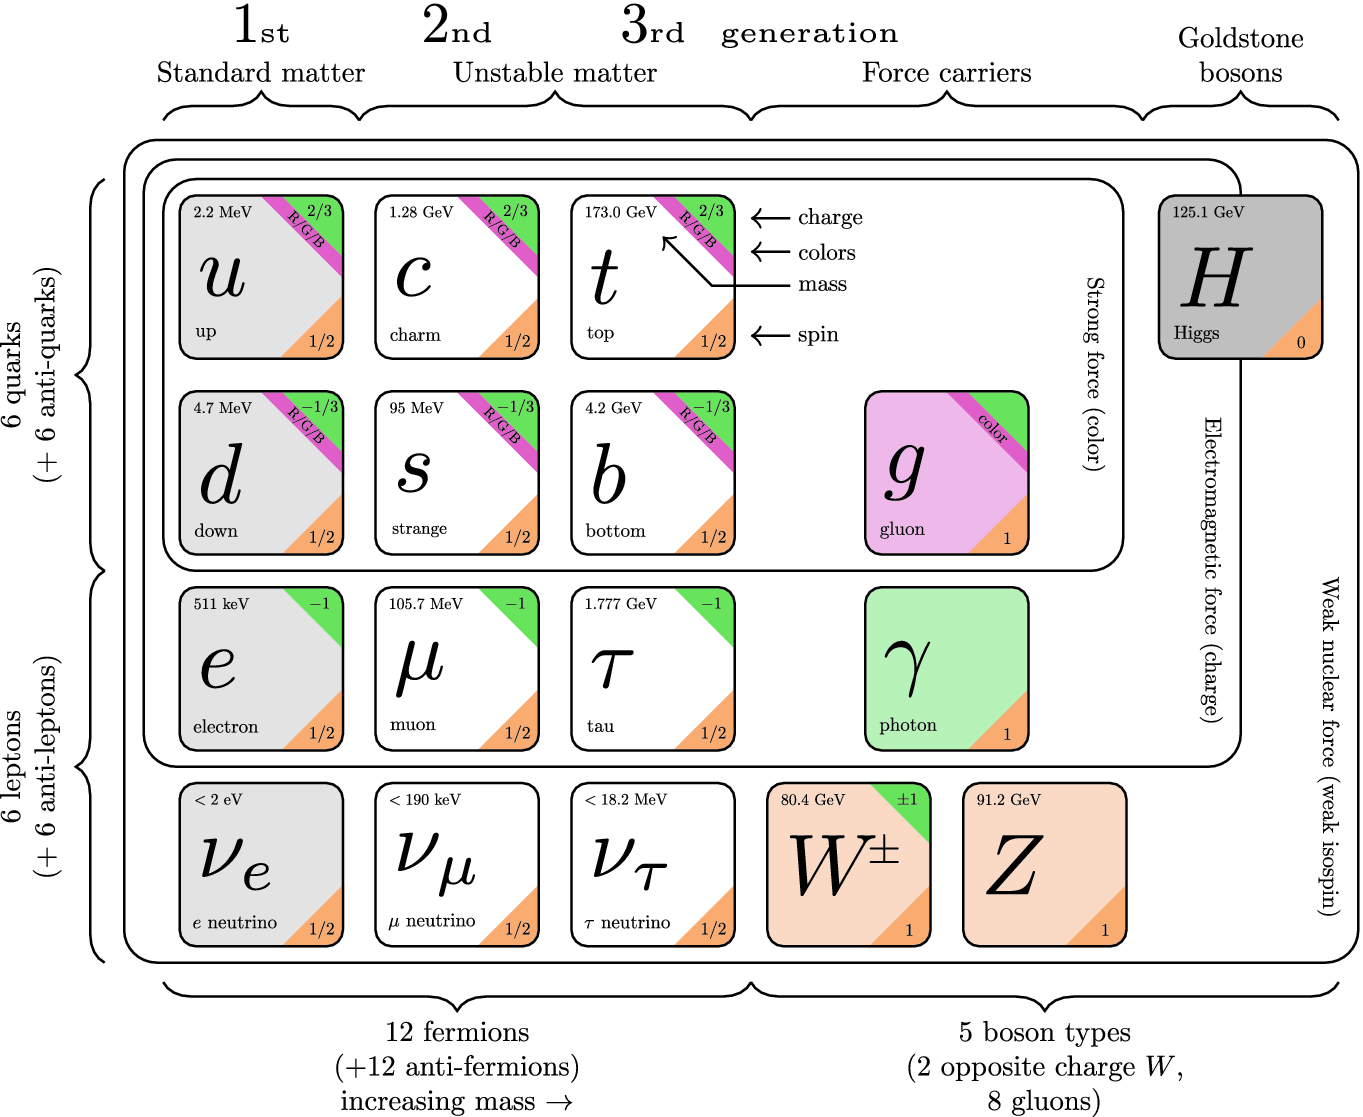
\includegraphics[width=5cm, height=4.2cm]{figs/SMFermions.png}
\end{minipage} \hfill \vfill

\begin{exampleblock}{} Muons \end{exampleblock}
\begin{itemize}
	\justifying
	\item Muons $\mu^-$ are one of the 12 fundamental particles existing
	\item They have a relatively small interaction cross-section with ordinary matter, allowing them to cross material without being stopped, making them interesting.
\end{itemize} \vfill
\end{frame}


\begin{frame}{Cosmic rays}
\justifying
Comic rays are a \textbf{constant flux of high energy particles} reaching the Earth:
\begin{itemize}
	\justifying
	\item Mostly made out of protons and atomic nuclei
	\item Trigger a decay chain by interacting with the atmosphere, producing muons

	\begin{minipage}[c]{.98\textwidth}
	\begin{center}
	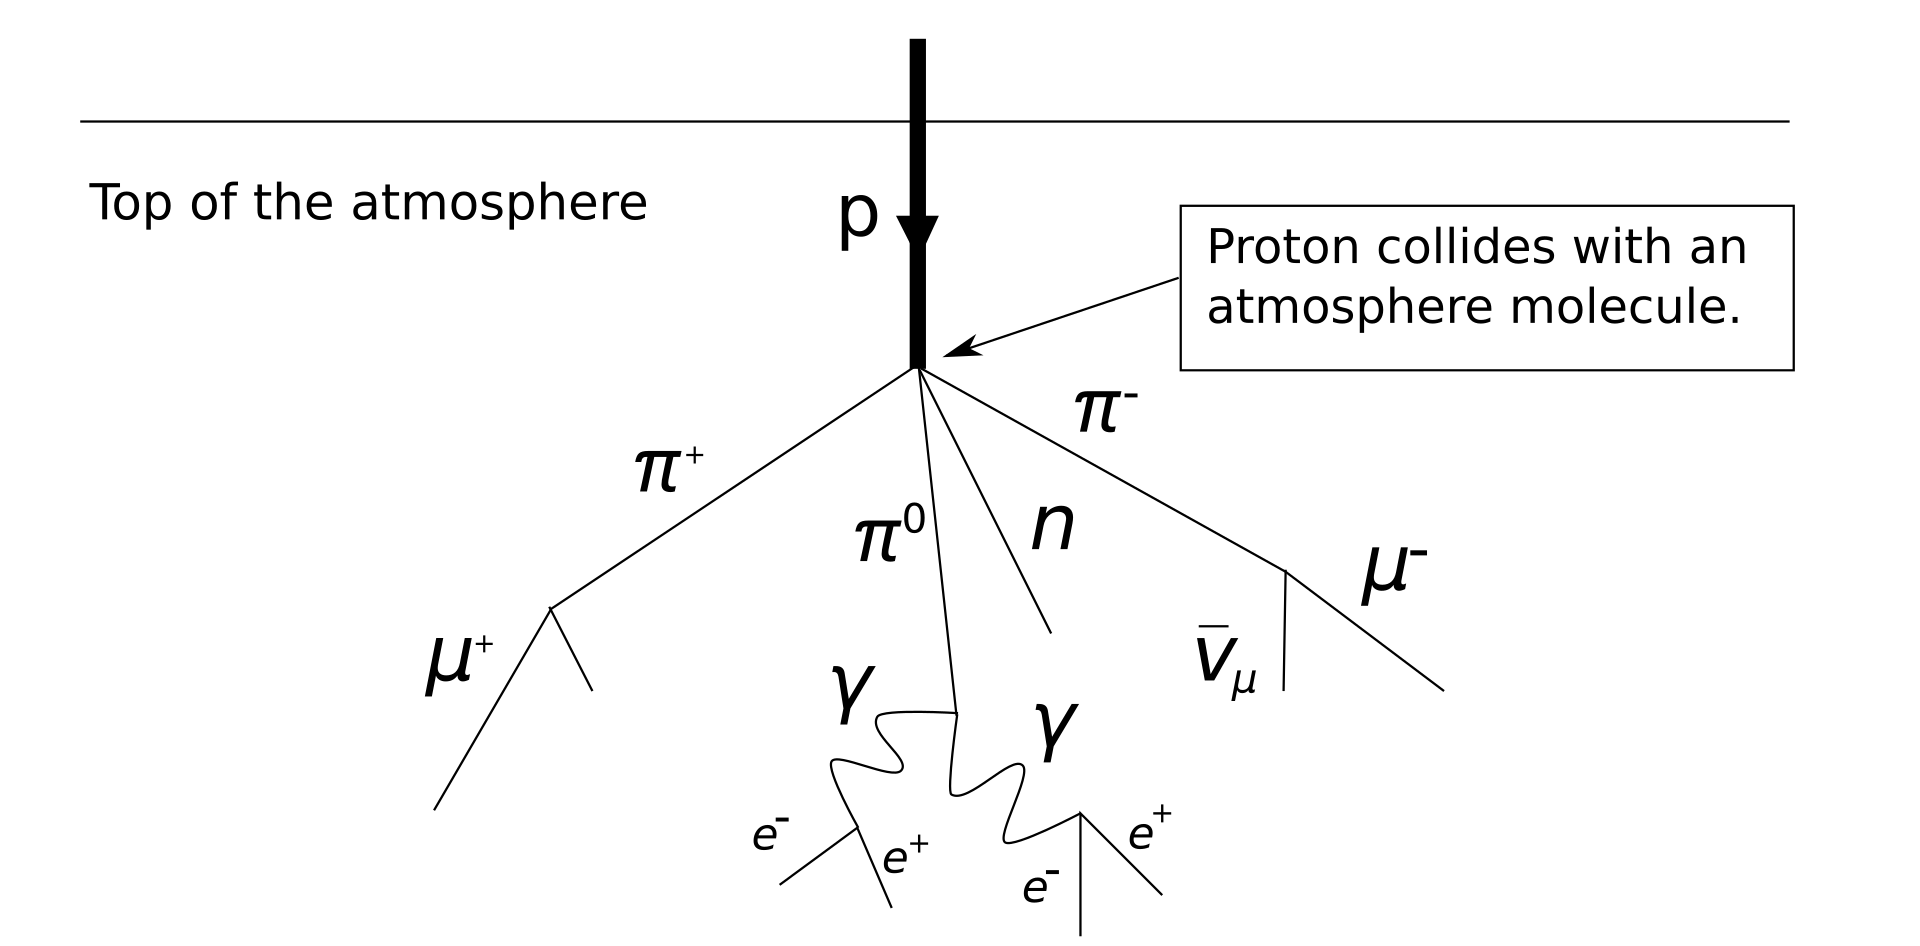
\includegraphics[width=8cm, height=4cm]{figs/cosmic.png}
	\end{center}
\end{minipage} \hfill 
	
	\item Muons are not stable ($\tau \simeq 2.2\mu$s) but relativistic effects makes some of them live long enough to reach the ground \\ \hspace{10pt} $\rightarrow$ 10.000 cosmic muons per $m^2$ and per minute are observed at sea level.
\end{itemize} \vfill

\end{frame}

\begin{frame}{Muons interactions with matter}
\justifying
%Muons interact with matter through two main processes:
\begin{exampleblock}{} Ionization \end{exampleblock}
When  the  incident  muon collides and gives some of its energy to the electrons of the absorber, but quite small for MIPs such as cosmic muons. \\
\hspace{10pt} $\rightarrow$ Basis for the \textbf{\alert{absorption muography}}, not covered here. \vfill

\begin{exampleblock}{} Multiple Coulomb scattering \end{exampleblock}
Coulomb interactions induce a \alert{\textbf{stochastic deviation}} whose central angular deviation can be described by a Gaussian of width $\theta_0$ under our experimental conditions:

\begin{minipage}[c]{.48\textwidth}
\begin{equation*}
\label{eq:Moliere}
\theta_0 \simeq \frac{13.6 \text{ MeV}}{\beta c p} \sqrt{\frac{x}{X_0}}
\end{equation*}

\justifying
The deviation depends on the number of radiation lengths $X_0$ and on the medium crossed. \\
\hspace{10pt} $\rightarrow$ Basis for the \textbf{\alert{scattering muography}}.
\end{minipage} \hfill
\begin{minipage}[c]{.51\textwidth}
	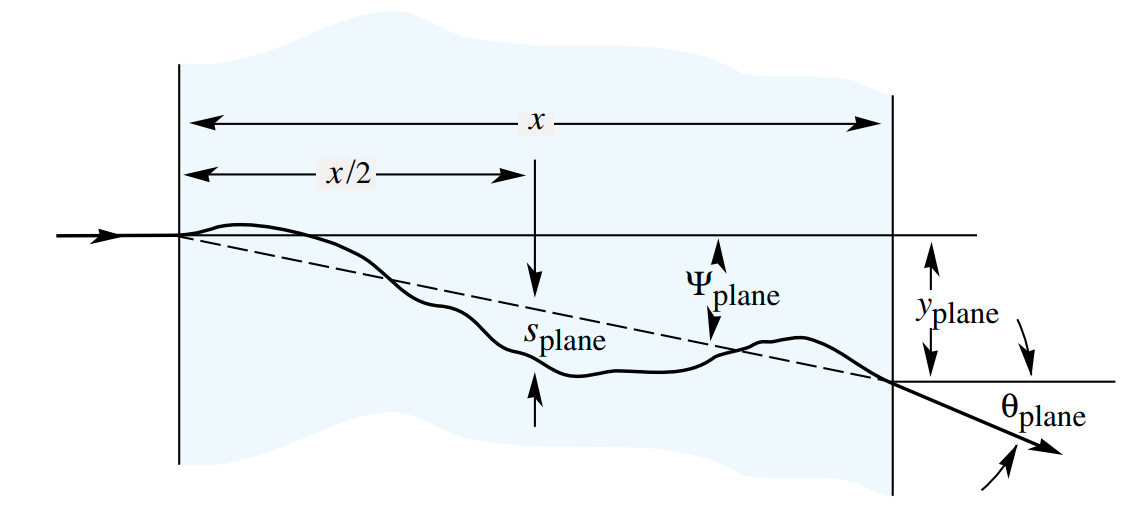
\includegraphics[width=6.3cm, height=2.6cm]{figs/moliere.png}
\end{minipage} \hfill \vfill
\end{frame}

\begin{frame}{Muon tomography}
Instead of \textit{calculating} the deviation expected for a cosmic muon, we can \textit{measure} the positional and angular deviation suffered \textbf{to estimate the properties of the medium crossed}. \vfill
% \\ \hspace{10pt} $\rightarrow$ Main idea behind the principle of \textbf{\alert{muon tomography}}, or \textbf{\alert{muography}}. \vfill

Several advantages over other imaging techniques:
\begin{itemize}
\justifying
\item Non-destructive technique
\item High penetrating capabilities allowing to probe large and dense objects
\item Completely safe, by using natural cosmic rays for the measurement.
\end{itemize} \vspace{10pt}

\begin{minipage}[c]{.54\textwidth}
\justifying

	Muography can be used in many different fields:
\begin{itemize}
	\justifying
	\item Find hidden rooms in Pyramids
	\item Nuclear waste/facilities inspection
	\item In volcanology, to know whether a pocket is empty or full of lava.
\end{itemize}	
	
\end{minipage} \hfill
\begin{minipage}[c]{.44\textwidth}
	\begin{center}
	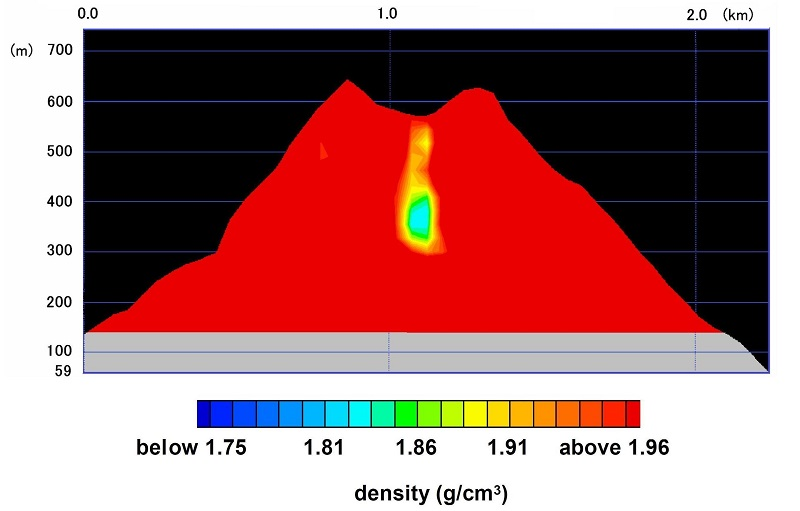
\includegraphics[width=5cm, height=3.5cm]{figs/volcano.jpg}
	\end{center}
\end{minipage} \hfill \vfill
\end{frame}








%Statistical basis
\begin{frame}{}
\centering
	\huge{\textbf{\color{mycolor} Section II}} \newline
	\LARGE{\textbf{\color{mycolor} Statistical basis \color{black}}} \vfill
\Large{The algorithm developed heavily relies on several important statistical concepts that we can now define.} \vfill
\end{frame}

\begin{frame}{Probability density functions}

\begin{minipage}[c]{.50\textwidth}
\justifying
PDFs are mathematical expressions defining probability distributions \textbf{which represent the likelihood of any given outcome}. \\ \vspace{10pt}
The area below the PDF in an interval can be interpreted as the value of the probability of a random variable X occurring. 
\end{minipage}
\begin{minipage}[c]{.50\textwidth}
\begin{center}
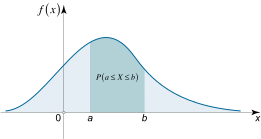
\includegraphics[width=5cm, height=2.2cm]{figs/PDF.png}
\end{center}
\end{minipage} \vfill

\begin{minipage}[c]{.50\textwidth}
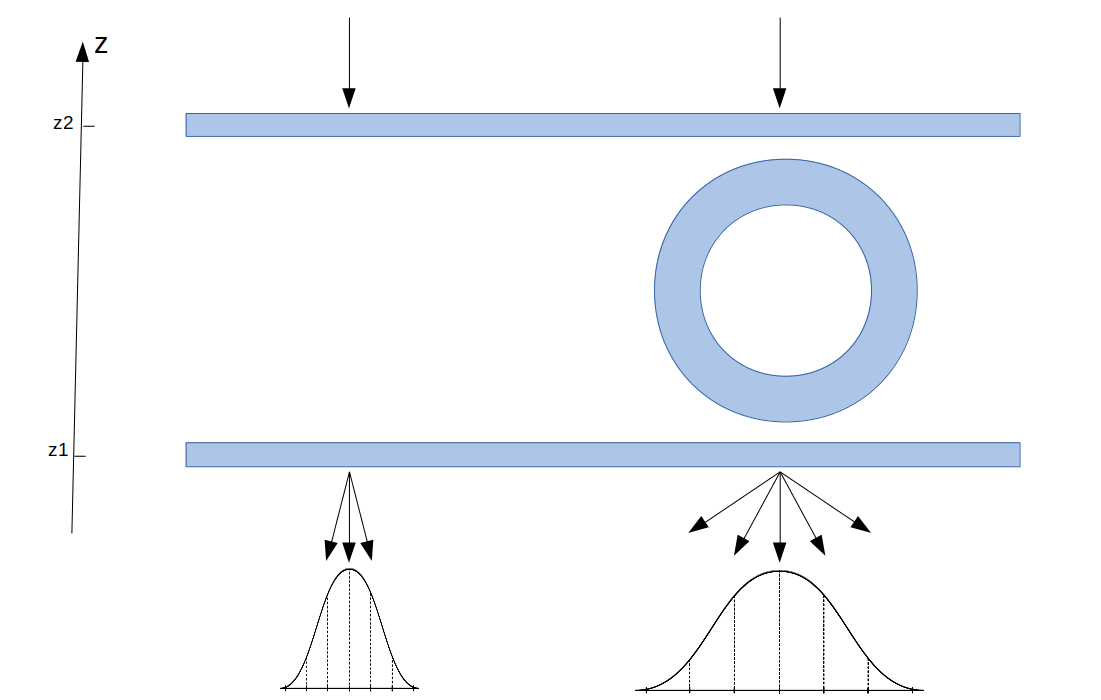
\includegraphics[width=6cm, height=3.5cm]{figs/pdfs.png}
\end{minipage}
\begin{minipage}[c]{.50\textwidth}
\justifying
The multiple scattering is a stochastic process, making PDFs extremely important. 

\begin{exampleblock}{}
\justifying A thicker and denser object results in a statistically higher expected deviation and a larger standard deviation $\sigma$ of the Gaussian PDF. \end{exampleblock}

%\\ \vspace{10pt}
%The study of the $\sigma$ of the deviation will then allow us to determine the thickness of the pipe placed between the detectors.
\end{minipage}
\end{frame}

\begin{frame}{Kernel density estimation}
This method allows us to estimate the shape of an unknown PDF $f$ of a random variable $X$ from a set of $N$ observations.

\begin{minipage}[c]{.50\textwidth}
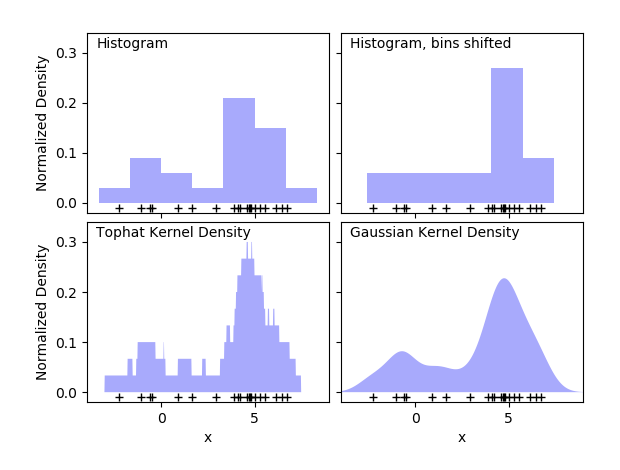
\includegraphics[width=5.8cm, height=5cm]{figs/kernels.png}
\end{minipage}
\begin{minipage}[c]{.50\textwidth}
\justifying
The usual way to proceed is to simply put the observations in an histogram, but this results in a non continuous function with possible gaps. \\ \vspace{10pt}
We then define $\hat{f}_h(x)$, an estimator of $f$ defined as the sum of continuous functions instead.

\begin{equation*}
\label{eq:KDF}
\hat{f}_h(x) = \frac{1}{Nh} \sum_{i=1}^{N} K \left (\frac{x-x_i}{h} \right )
\end{equation*}
\end{minipage}

Two important parameters
\begin{itemize}
\item The \textbf{\alert{kernel}} $K$, chosen as Gaussian functions in this case
\item And the \textbf{\alert{bandwidth}} $h$, a smoothing parameter.
\end{itemize} \vfill

\end{frame}

\begin{frame}{Monte-Carlo simulations}
\justifying
Monte-Carlo simulations are obtained from algorithms developed to \textbf{compute approximate numerical values to stochastic problems} using random processes and probabilistic techniques. \vfill

Instead of relying on actual data collected from the experiment, we can:
\begin{enumerate}
\justifying
\item Use CRY, a cosmic ray generator to simulate thousands of incident muons
\item Make these muons go through a complete simulation of the detector done with Geant4
\item Go through the same post-processing process as actual data
\item Build the PDF for a given experiment from these simulations
\item Repeat this experiment $N_\text{MC}$ times, \textbf{simulating thousands of experiments} without the need to perform them.
\end{enumerate} \vfill

Simulating an experiment is cheaper and faster than running it and allows to compare results obtained from both channels. In this work, the dependence on Geant4 will be removed as well, to make this process even faster. \vfill
\end{frame}

\begin{frame}{Maximum likelihood estimation}
\justifying
We still need a method allowing us to \textbf{estimate the optimal geometrical parameters of an object from a given set of measurements}, such as the thickness of a pipe. \vfill

\begin{exampleblock}{}
\justifying 
The likelihood measures the goodness of a fit with respect to a sample of data for one or several unknown parameters. If $\bm \theta$ are the parameters of the model and $x$ is the measurement of a random variable $X$ defined from a PDF $f$, then:
\begin{equation*}
\label{eq:likelihood}
\mathcal{L}(\bm \theta | x) = f_{\bm \theta}(x) = P(X = x | \bm \theta)
\end{equation*}
 \end{exampleblock} \vfill

The likelihood can be described as an hypersurface whose peak gives the optimal set of parameters maximizing the probability of drawing the actual sample measured $\rightarrow$ the objective is to \textbf{find the set of parameters minimizing the log-likelihood} $l(\bm \theta | x) = -2 \log(\mathcal{L}(\bm \theta | x))$. \vfill

In this work, the parameter to be optimized will be the thickness of a steel pipe. \vfill
\end{frame}








%The algorithm
\begin{frame}{}
\centering
	\huge{\textbf{\color{mycolor} Section III}} \newline
	\LARGE{\textbf{\color{mycolor} Algorithm implementation \color{black}}} \vfill
\Large{A C++ framework has been developed in order to solve this problem, relying on two main parts: a PipeReconstructor and a Generator, both described in the next slides.} \vfill
\end{frame}

\begin{frame}{General idea}
\begin{exampleblock}{} PipeReconstructor \end{exampleblock}
\justifying
General set of classes defined in the next slides allowing us to:
\begin{itemize}
\justifying
\item Define the geometry of the problem (mainly, the detector and object position and size)
\item Compute the intersection points between cosmic muons and this geometry
\item Propagate these muons through the geometry using the multiple scattering
\item Calculate the likelihood of a given measurement for a given geometry
\item Finally, find the optimal object parameters from this likelihood.
\end{itemize} \vfill

\begin{exampleblock}{} Generator \end{exampleblock}
\justifying
Another class allowing us to generate muons by performing Monte-Carlo simulations using some of the functions of the PipeReconstructor and without relying on Geant4. \vfill

%\begin{exampleblock}{} Plotter \end{exampleblock}
%\justifying
%Simple set of scripts used in order to plot all the results shown in the next slides. \vfill
\end{frame}

\begin{frame}{Surfaces, volumes and MuonStates}
\justifying
\begin{minipage}[c]{.65\textwidth}
\begin{exampleblock}{} Surfaces and Volumes \end{exampleblock}
\justifying
General virtual classes defining the geometry of the problem ; a Volume is defined as a vector of a fixed number of Surfaces. \\ \vspace{5pt}
In particular, the subclasses Cylinder and Pipe are mostly used in this work. A Pipe is defined from 7 parameters: 
\begin{itemize}
\item Its central position ($x$, $y$, $z$)
\item Its inner $r$ and outer radii $R$
\item Its constant density $\rho$
\item And its length $L$ along the axis of the cylinder.
\end{itemize}
\end{minipage}
\begin{minipage}[c]{.33\textwidth}
\vspace{35pt}
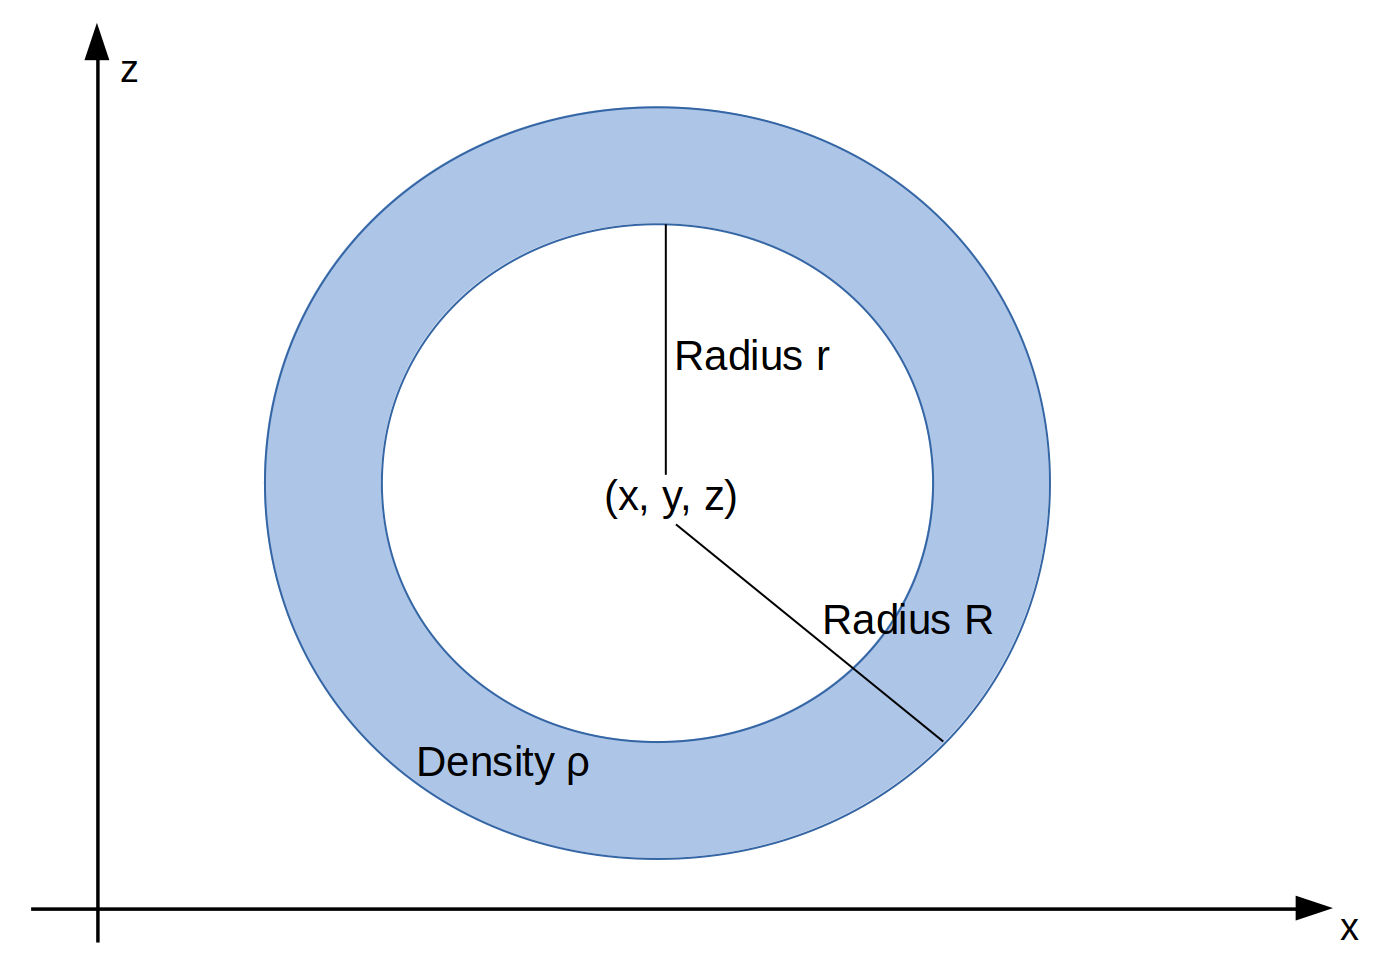
\includegraphics[width=4.5cm, height=3.2cm]{figs/cylinder.png}
\end{minipage} \vfill
\begin{exampleblock}{} MuonStates \end{exampleblock}
A MuonState is a class defining a muon from two vectors representing its position ($x$, $y$, $z$), direction ($v_x$, $v_y$, $v_z$) and momentum value $p$. \\ \vspace{10pt}

%Two MuonStates are defined for each experiment: one measured at the top detector ($x_1$, $y_1$, $z_1$, $v_{x1}$, $v_{y1}$, $v_{z1}$, $p_1$), and one at the bottom, with the index 2. \vfill
\end{frame}

\begin{frame}{Propagator}
\justifying
The propagator is the object allowing to \textbf{propagate a MuonState through a Volume}: \vfill

\begin{minipage}[c]{.59\textwidth}
\begin{enumerate}
\justifying
\item First, the distances between a MuonState and all the Surfaces of the Volume are computed and the first intersection point is kept \vspace{5pt}
\item The muon is propagated 90\% of the distance to this cut point using the multiple scattering, and this process is repeated several times until being closer to 0.1mm to the first surface \vspace{5pt}
\item The Surface is manually crossed by slightly moving the MuonState along its direction \vspace{5pt}
\item This process is repeated for all the Surfaces of the Volume and then one last time until reaching the bottom detector, where the MuonState is returned.
\end{enumerate}
\end{minipage}
\begin{minipage}[c]{.40\textwidth}
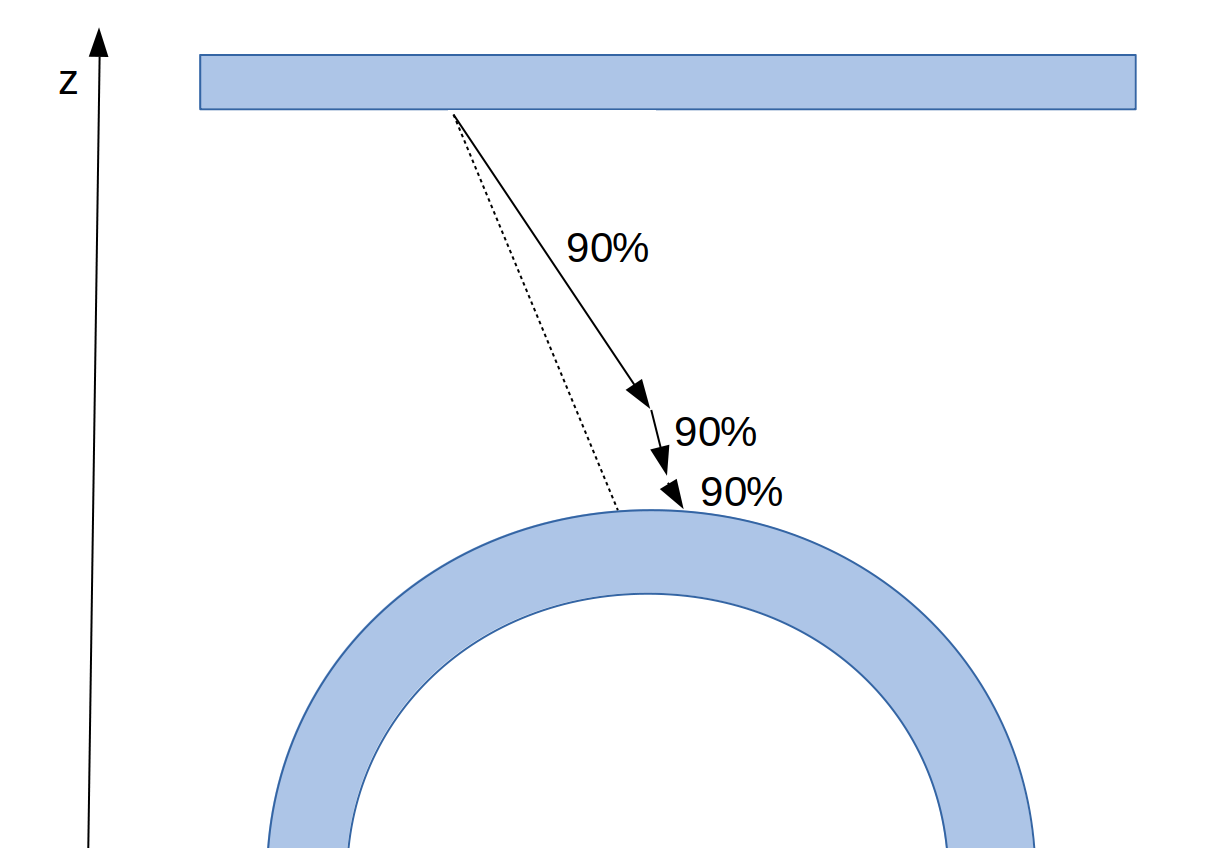
\includegraphics[width=4.5cm, height=3.2cm]{figs/propagation.png}
\end{minipage} \vfill

Eventual muons which do not actually cross the pipe or out of the acceptance of any of the detectors are rejected at this stage. \vfill
\end{frame}

\begin{frame}{Likelihood}
\justifying
The Likelihood class takes as input a Volume and a data/MC rootfile, to tell us \textbf{how likely it is that we obtained exactly these measurements for the geometry given}: \vspace{5pt}

\begin{enumerate}
\begin{minipage}[c]{.58\textwidth}
\item First, four MuonStates are computed:
	\begin{itemize}
	\justifying
	\item The IncomingMuon and OutgoingMuon, as the actual measurements made by the top/bottom detectors
	\item The IncomingMuonLinearDown, the linear propagation of the IncomingMuon, used as reference
	\item And the IncomingMuonDown, by propagating the initial state with our Propagator through the Volume
	\end{itemize}
\end{minipage}
\begin{minipage}[c]{.36\textwidth}
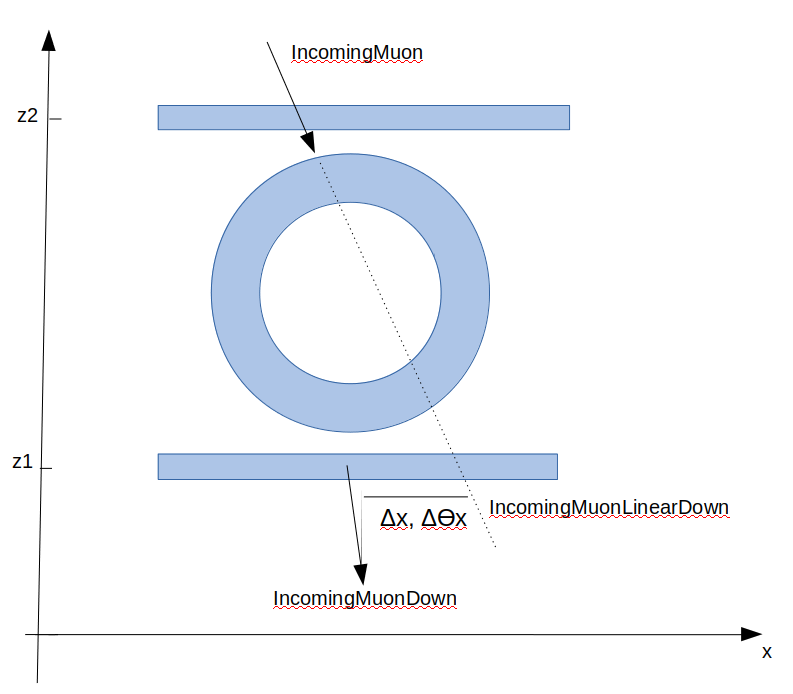
\includegraphics[width=4.2cm, height=3.15cm]{figs/parameters.png}
\end{minipage} \vspace{5pt}

\justifying
\item This process is repeated $n_{\text{iter}}$ times for each input event, obtaining each time values for the $\Delta$x, $\Delta \theta_x$, $\Delta$y and $\Delta \theta_y$ parameters, filling 2 bi-dimensional PDFs histograms \vspace{5pt}
\item The histograms obtained are smoothen using the kernel density estimation method \vspace{5pt}
\item The probability to observe the actual measurement (OutgoingMuon) is computed, and summed over all the ${N_\text{MC}}$ events in the file, returning the value:

\begin{equation*}
\label{eq:totallikelihood}
\mathcal{L} = \sum_{i = 1}^{N_\text{MC}} -2.0 \left ( \log(\text{value}_{x, i}) + \log(\text{value}_{y, i}) \right)
\end{equation*}
\end{enumerate} \vfill
\end{frame}

%\begin{frame}{Generator}
%\justifying
%The Generator allows us to generate Monte-Carlo experiments in a faster way than using Geant4, which is more complex, relying on a complete description of the detector. \vfill
%
%Information from CRY is therefore used in order to simulate thousands of incident muons, read from a rootfile previously created by MuonSystems. Each incident muon is then propagated through a given Volume using the previous functions, therefore simulating thousands of experiments. \vfill 
%\end{frame}










%Results obtained
\begin{frame}{}
\centering
	\huge{\textbf{\color{mycolor} Section IV}} \newline
	\LARGE{\textbf{\color{mycolor} Results obtained \color{black}}} \vfill
\Large{First of all, the results obtained by our Generator whill be shown and compared to Geant4, before moving on to the actual results obtained with our algorithm.} \vfill
\end{frame}

\begin{frame}{Generator validation}
\justifying
The Generator allows us to generate Monte-Carlo experiments in a faster way than using Geant4, which is more complex, relying on a complete description of the detector. \\ \vspace{10pt}
The first step was then to validate our Monte-Carlo simulations by comparing measurements simulated by both Geant4 and our own Generator for a given geometry. \vfill

\begin{minipage}[c]{.32\textwidth}
\begin{exampleblock}{} \begin{center}Bottom X position\end{center} \end{exampleblock}
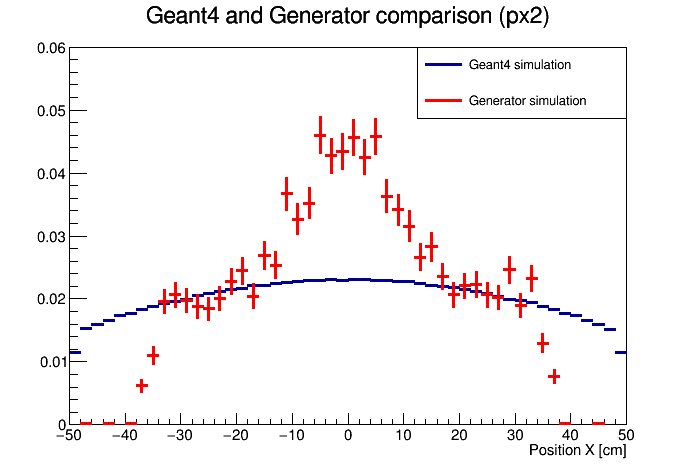
\includegraphics[width=4.2cm, height=3.2cm]{figs/px2-17p2vs17p2.png} 
\end{minipage}
\begin{minipage}[c]{.32\textwidth}
\begin{exampleblock}{} \begin{center}$\Delta_x$ parameter\end{center} \end{exampleblock}
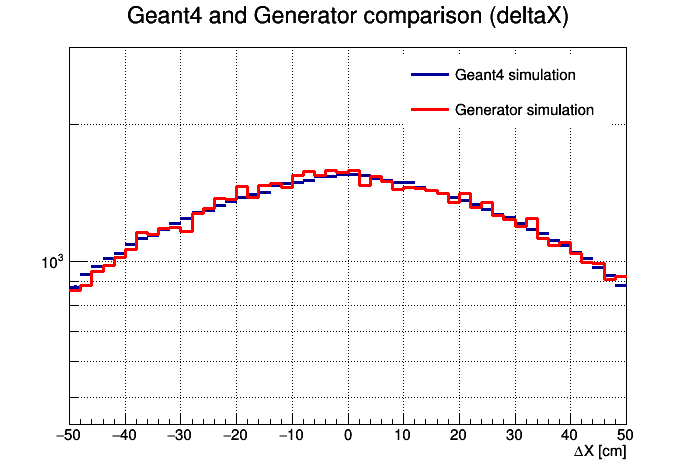
\includegraphics[width=4.2cm, height=3.2cm]{figs/deltaX-17p2vs17p2.png}
\end{minipage}
\begin{minipage}[c]{.32\textwidth}
\begin{exampleblock}{} \begin{center}$\Delta \theta_x$ parameter\end{center} \end{exampleblock}
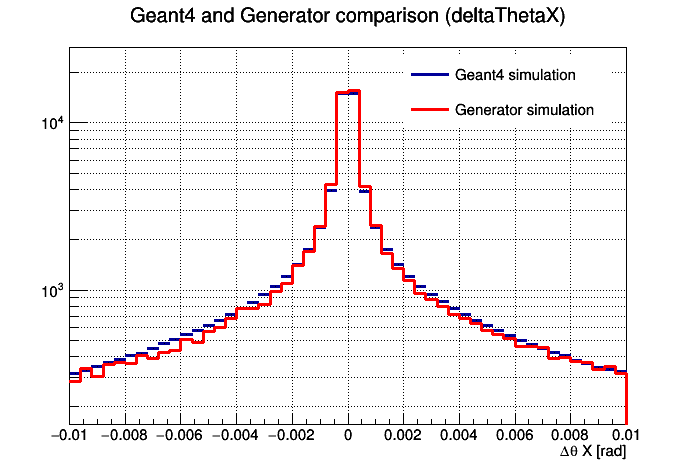
\includegraphics[width=4.2cm, height=3.2cm]{figs/deltaThetaX-17p2vs17p2.png}
\end{minipage}

\end{frame}

\begin{frame}{Pipes geometries}
\justifying
Once validated, 12 different Monte-Carlo files have been generated with our Generator with 10 to 50.000 events each, for different pipe geometries, having an outer radius of 20cm and inner radii ranging from 16.8 to 19.0cm. \vfill

\begin{figure}[htbp]
\centering
\begin{minipage}[b]{.49\textwidth}
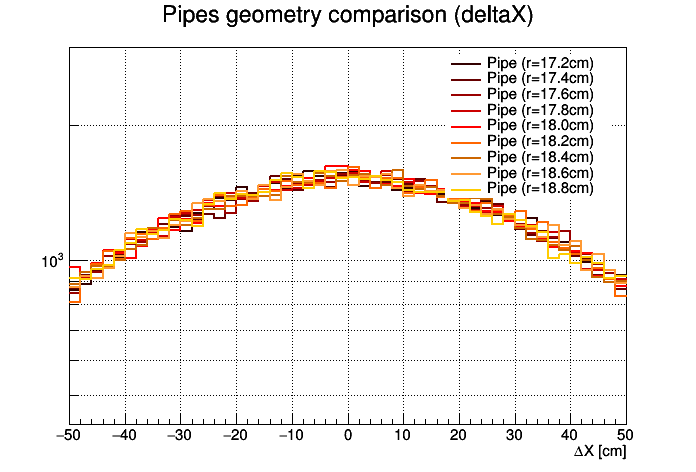
\includegraphics[width=6cm, height=4.8cm]{figs/deltaX.png}
\end{minipage}\hfill
\begin{minipage}[b]{.49\textwidth}
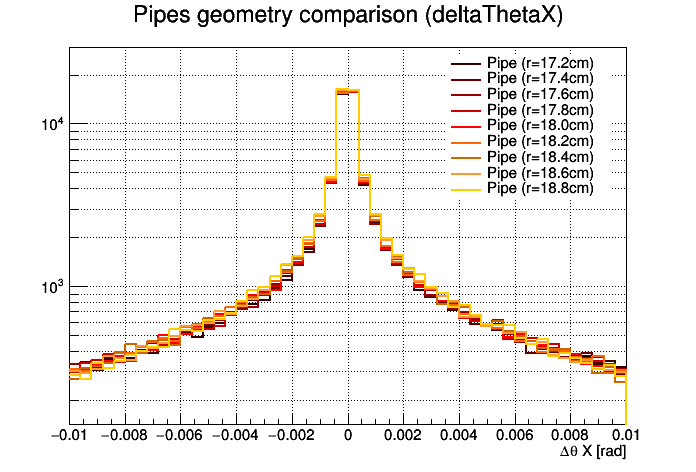
\includegraphics[width=6cm, height=4.8cm]{figs/deltaThetaX.png}
\end{minipage}\hfill
\label{fig:gemComp}
\end{figure} \vfill

It took 8 seconds to produce 50.000 events with our Generator, more than \textbf{two orders of magnitude faster} than a complete Geant4 simulation. \vfill
\end{frame}

\begin{frame}{Kernel density functions}
\justifying
Since the likelihood needs to be computed for every single event of the input simulation file by performing another computing extensive loop, the $n_{\text{iter}}$ parameter is kept as small as possible using the kernel density estimation method. \vfill
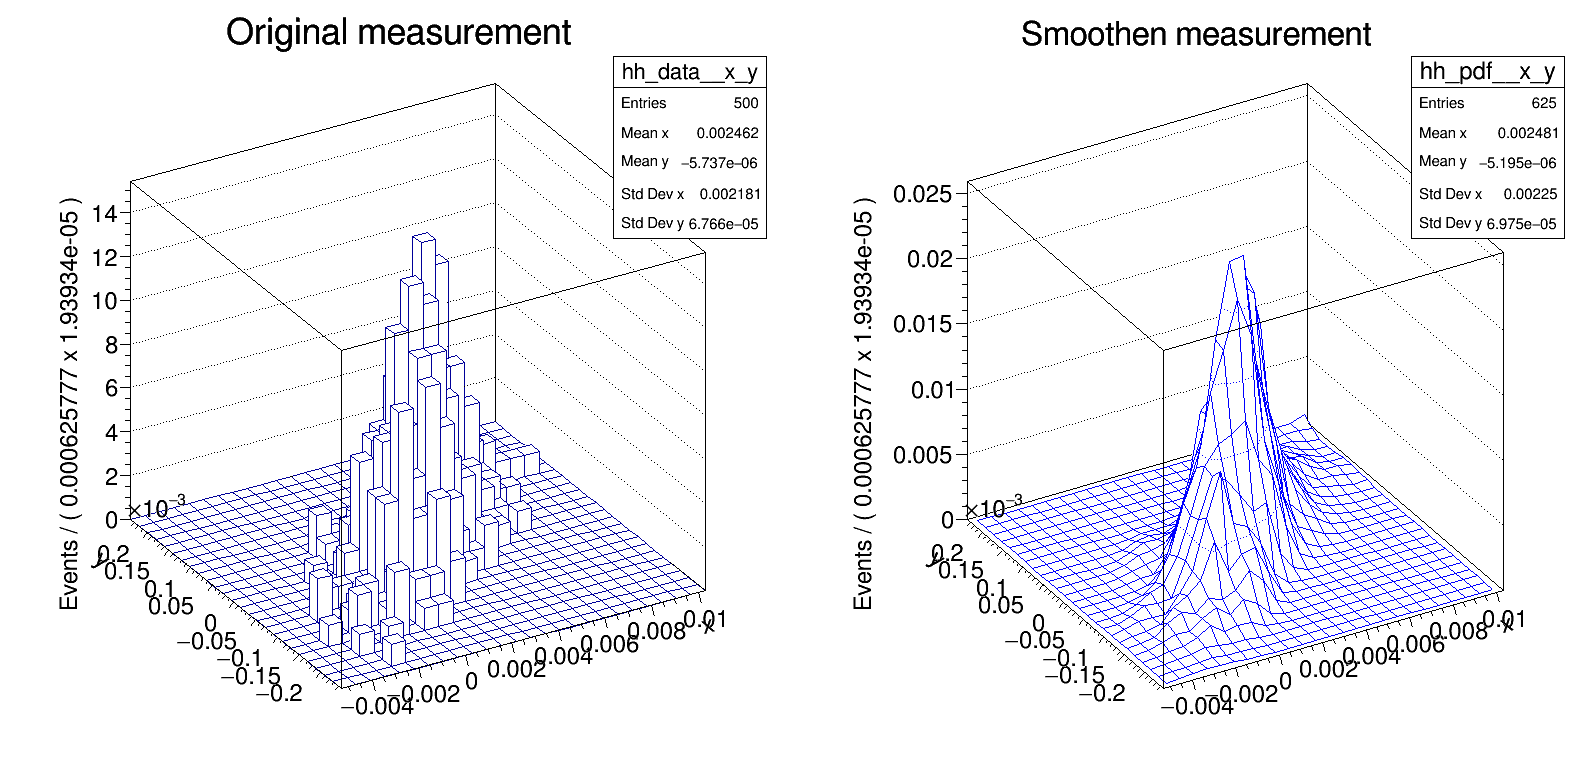
\includegraphics[width=12cm, height=5.5cm]{figs/plot_kernelx.png} \vfill
\end{frame}

\begin{frame}{Likelihood curves}
\justifying
Finally, we estimated the value of the total likelihood obtained for different pipe geometries, characterized by different inner radii, ranging from 16.6 to 19.0cm, by steps of 0.2cm. \vfill

The idea was to plot the likelihood obtained comparing one by one the generated file with the different geometries available and try to figure out which pipe geometry, in the x-axis, is more likely to give rise to the file considered. \vfill

\begin{minipage}[c]{.32\textwidth}
\begin{exampleblock}{} \begin{center}$r = 17.0$cm\end{center} \end{exampleblock}
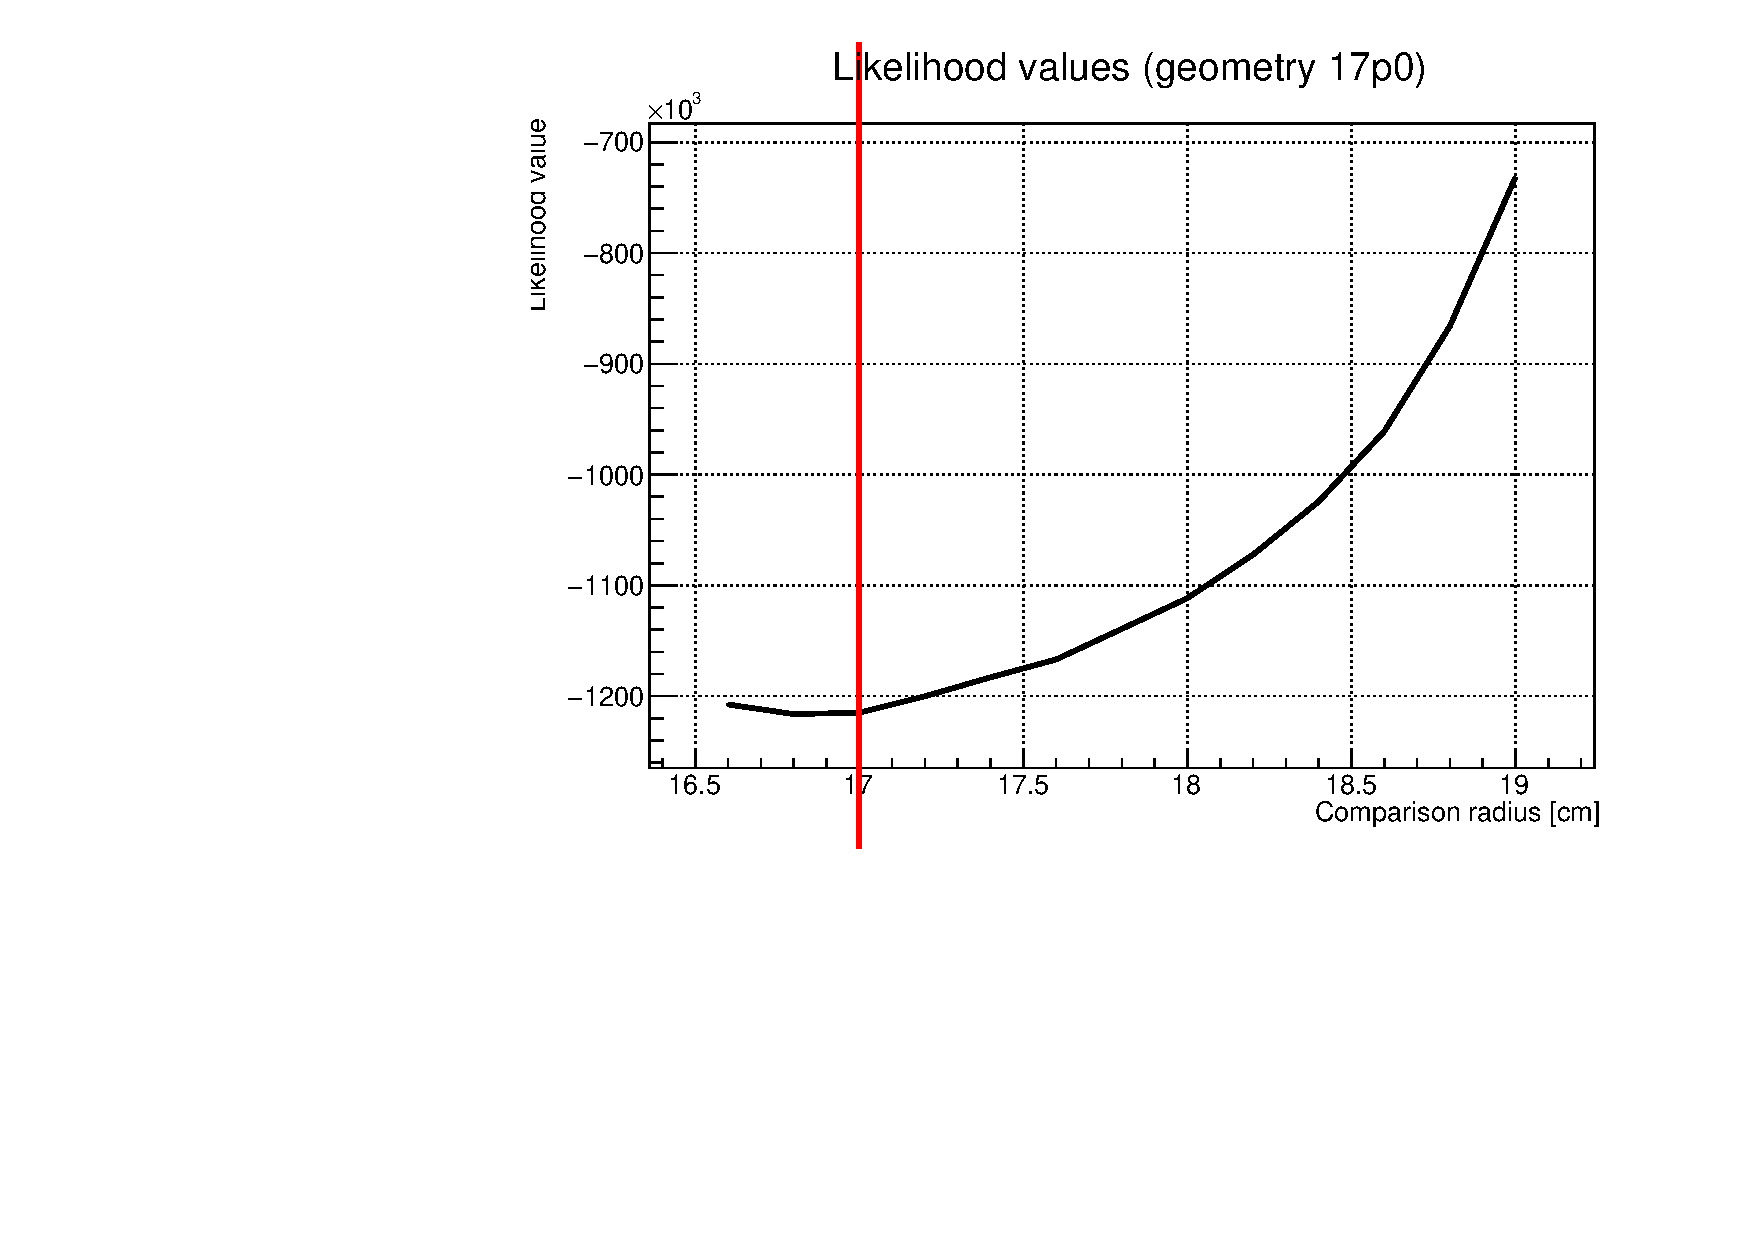
\includegraphics[width=4.2cm, height=3.2cm]{figs/likelihood100HighStat/likelihood17p0.pdf} 
\end{minipage}
\begin{minipage}[c]{.32\textwidth}
\begin{exampleblock}{} \begin{center}$r = 18.0$cm\end{center} \end{exampleblock}
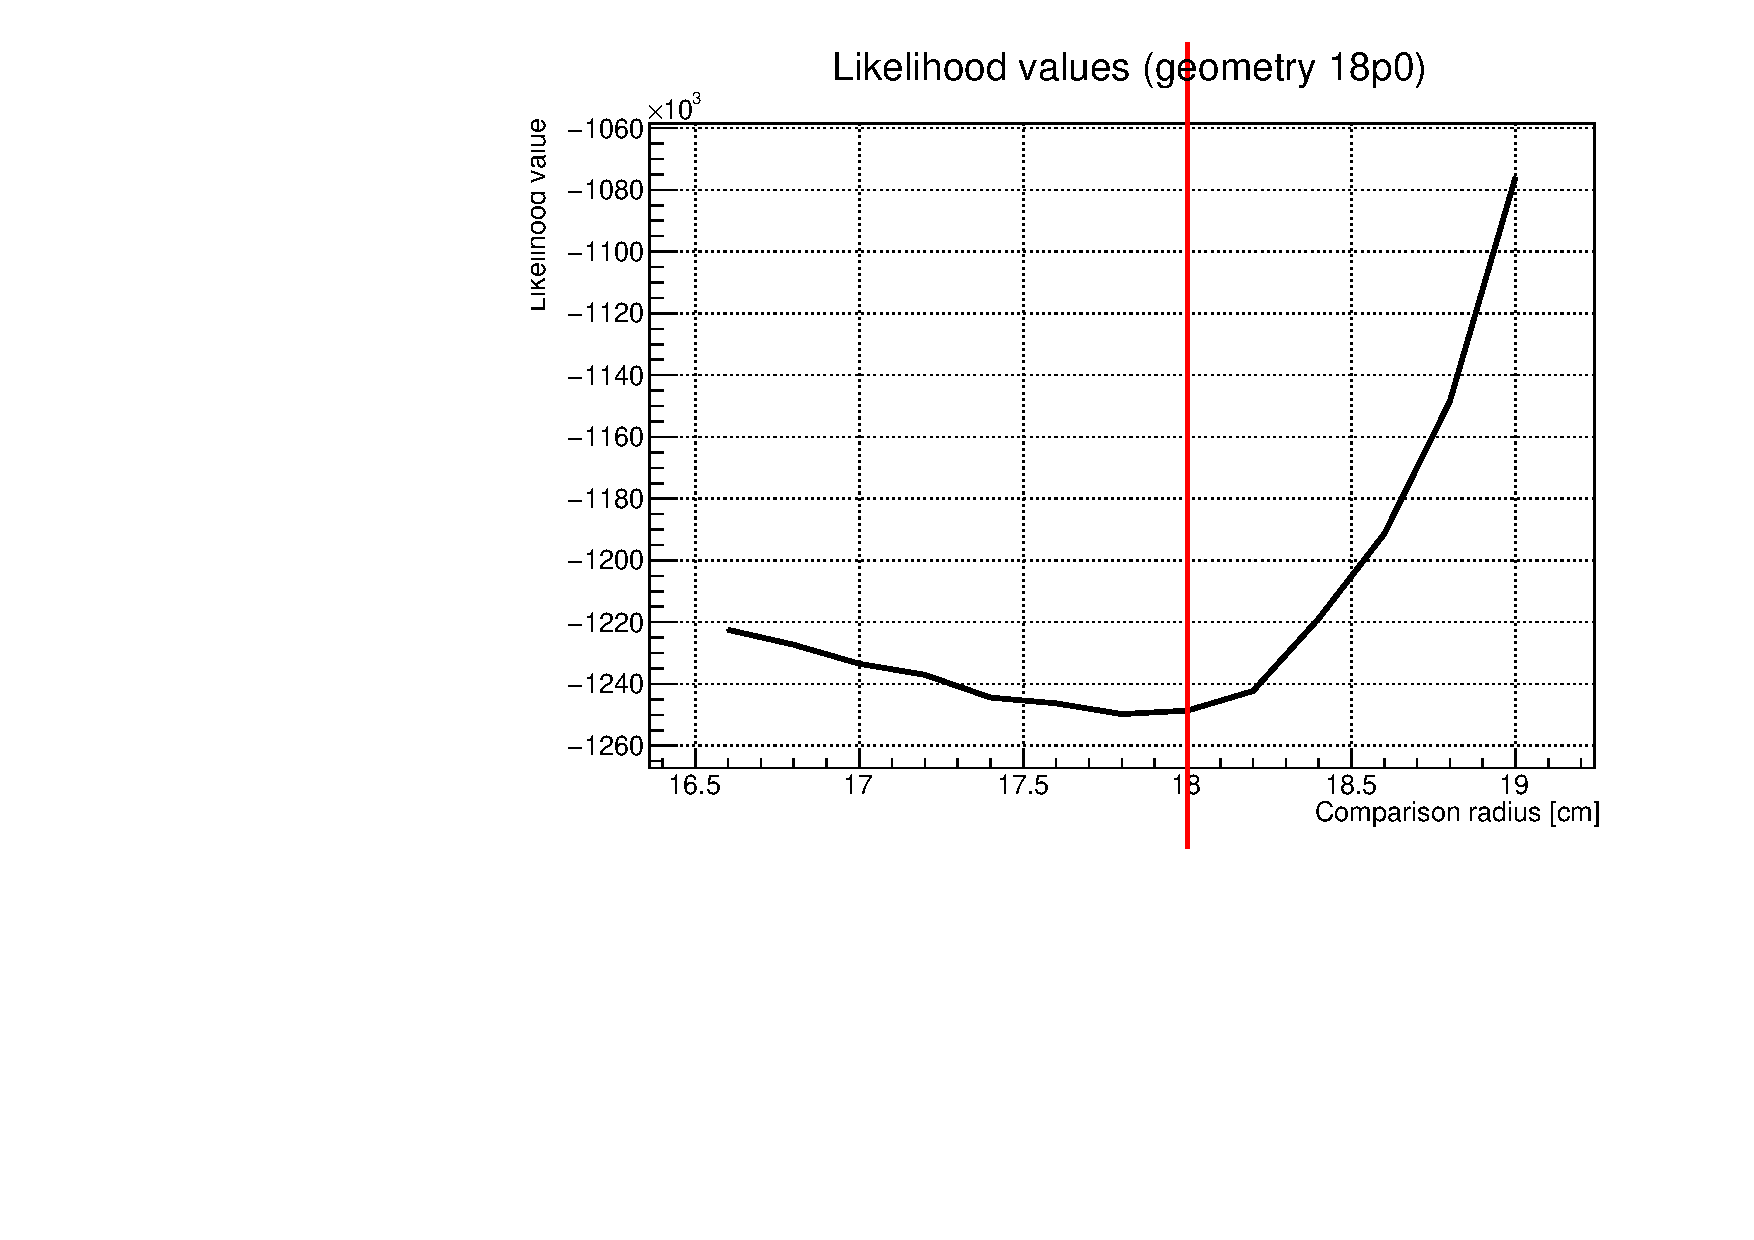
\includegraphics[width=4.2cm, height=3.2cm]{figs/likelihood100HighStat/likelihood18p0.pdf} 
\end{minipage}
\begin{minipage}[c]{.32\textwidth}
\begin{exampleblock}{} \begin{center}$r = 19.0$cm\end{center} \end{exampleblock}
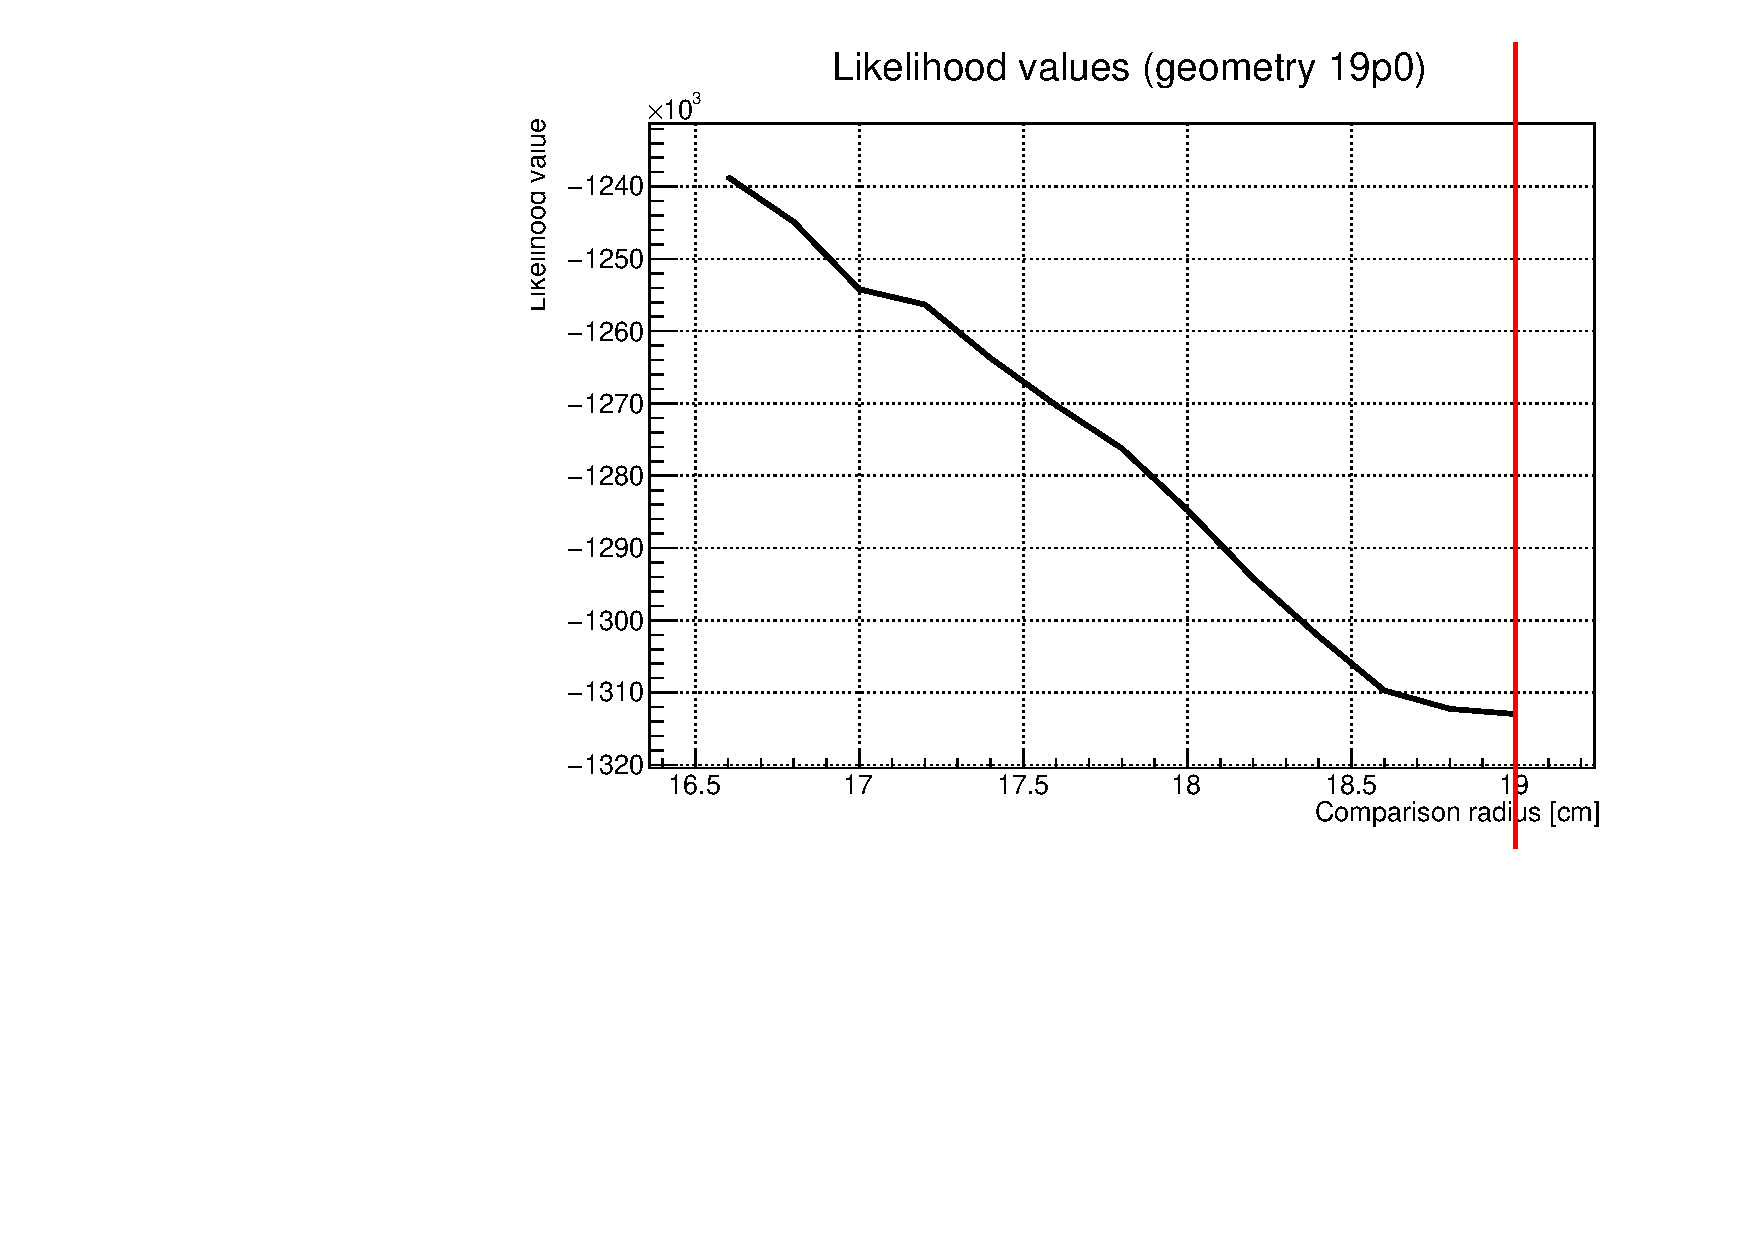
\includegraphics[width=4.2cm, height=3.2cm]{figs/likelihood100HighStat/likelihood19p0.pdf} 
\end{minipage} \vfill

We do observe the minimum exactly where it is supposed to be for most of the geometries, as seen in the backup. \vfill
\end{frame}

\begin{frame}{Likelihood curves}
\justifying
We also estimated the impact of the number of simulated events $n_{\text{MC}}$ and the number of likelihood computation iterations $n_{\text{iter}}$ on the likelihood curves, for the $r = 18.0$cm geometry. \vfill

\begin{minipage}[c]{.32\textwidth}
\begin{exampleblock}{} \begin{center}$n_\text{iter}$ = 100 \\ $n_\text{MC}$ = 10.000 \end{center} \end{exampleblock} \vspace{5pt}
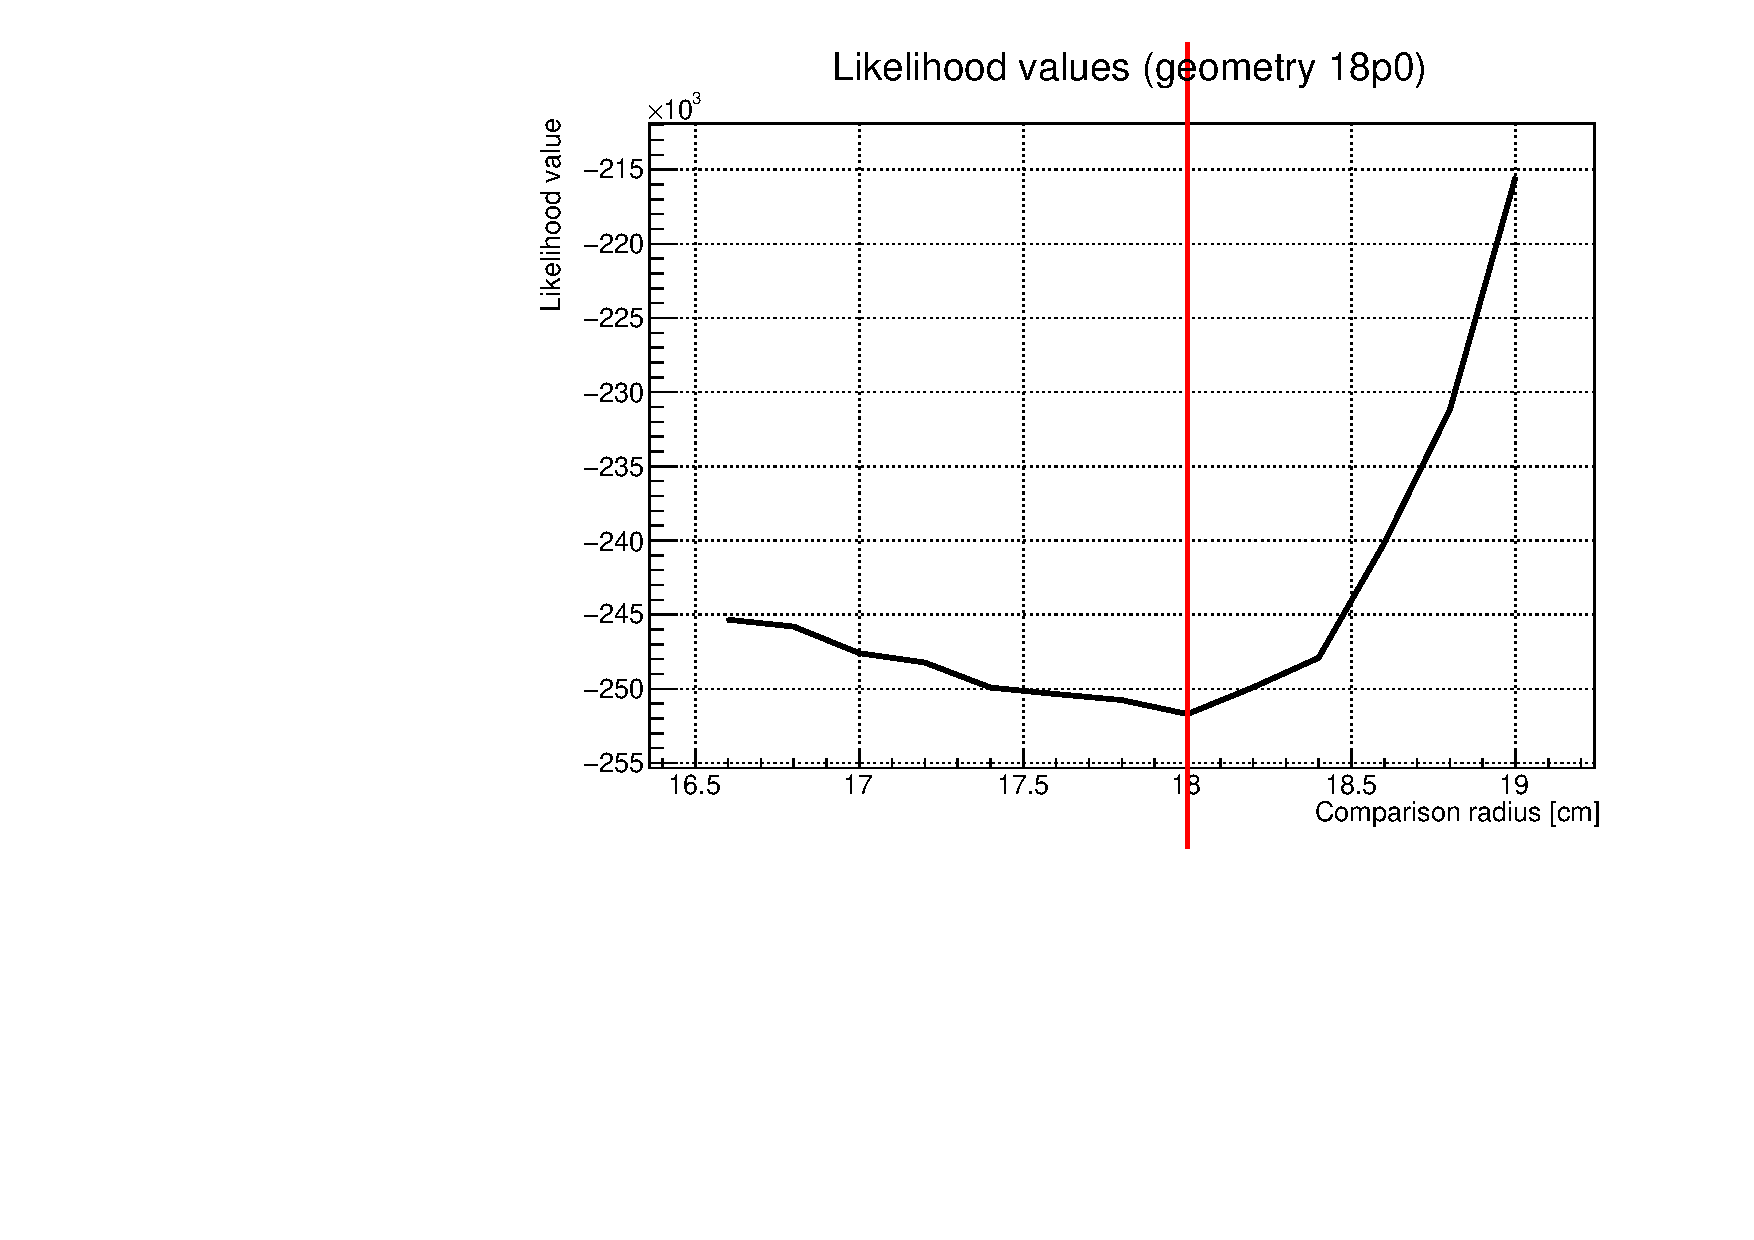
\includegraphics[width=4.2cm, height=3.2cm]{figs/likelihood100LowStat/likelihood18p0.pdf} 
\end{minipage}
\begin{minipage}[c]{.32\textwidth}
\begin{exampleblock}{} \begin{center}$n_\text{iter}$ = 100 \\ $n_\text{MC}$ = 50.000\end{center} \end{exampleblock} \vspace{5pt}
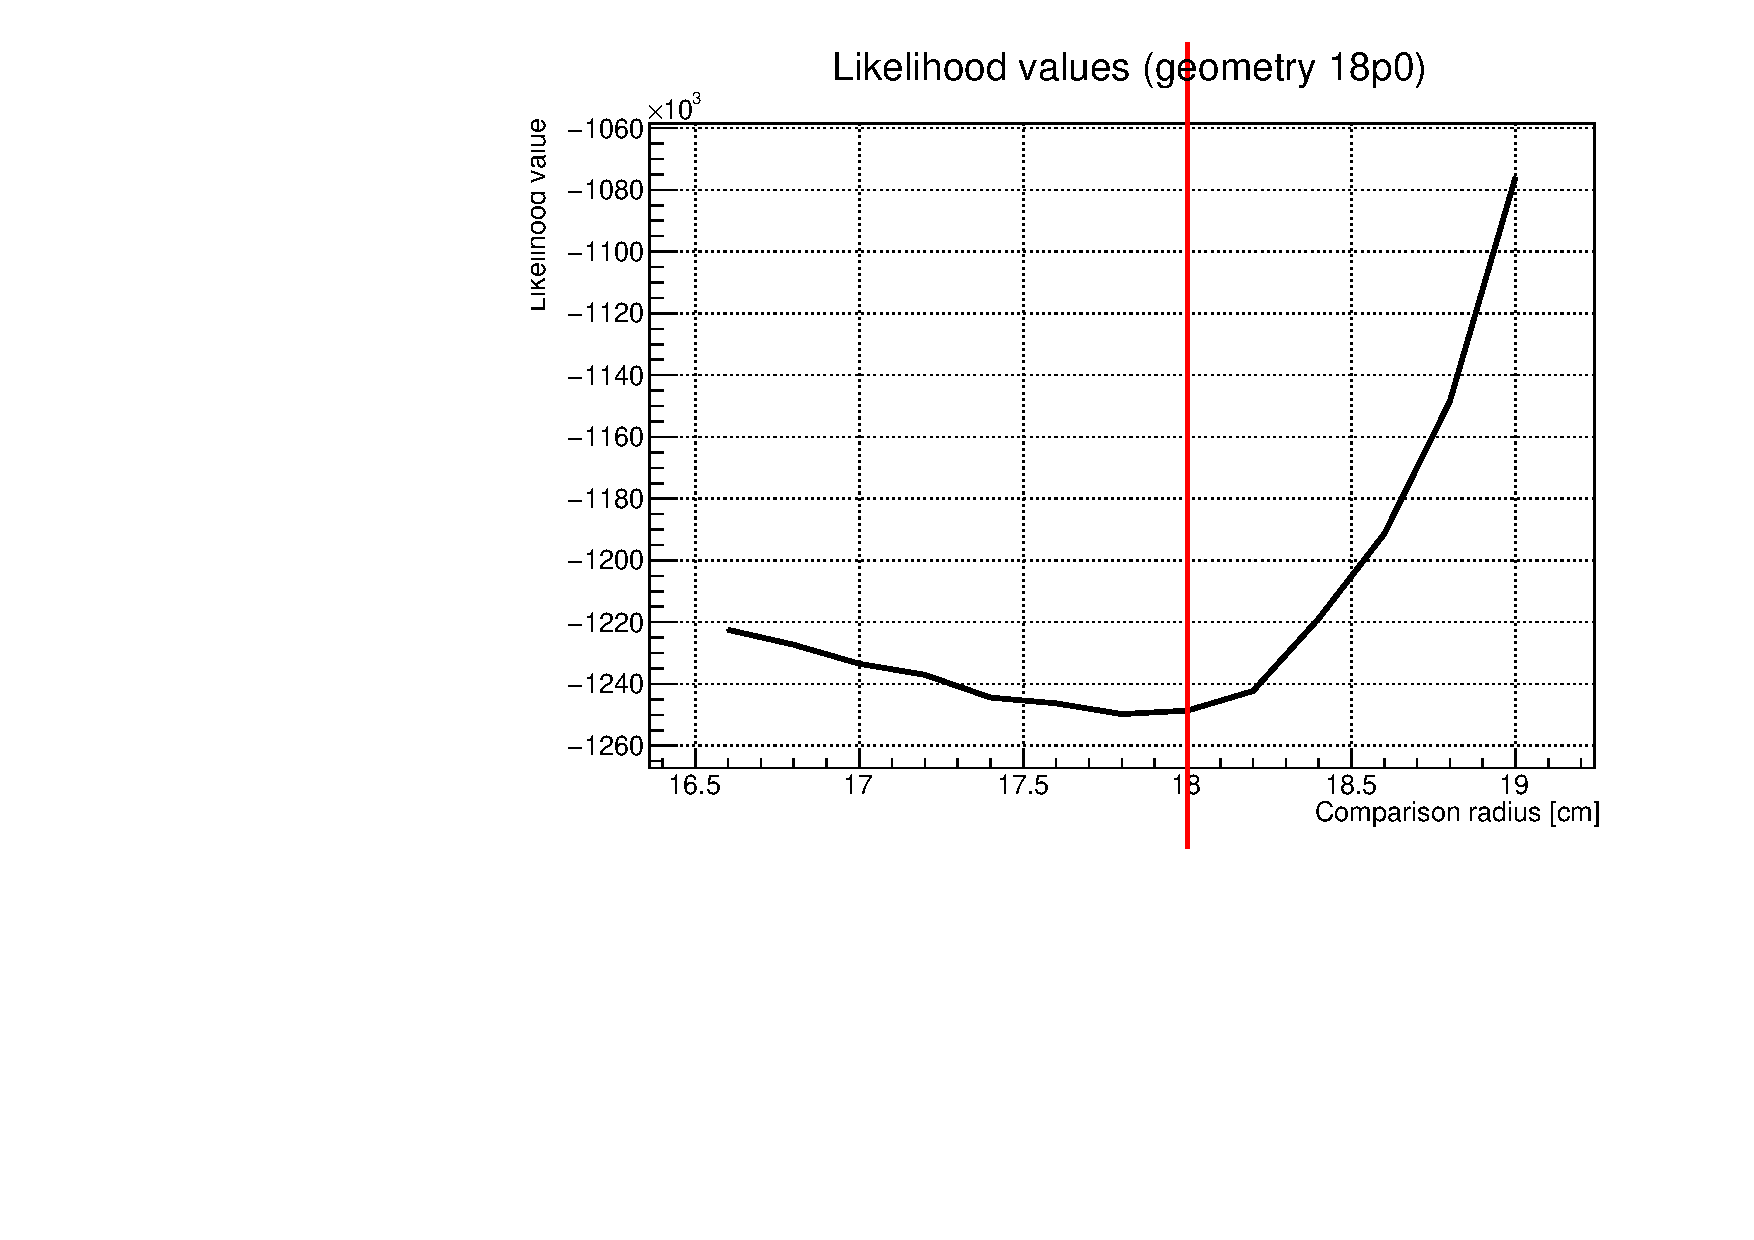
\includegraphics[width=4.2cm, height=3.2cm]{figs/likelihood100HighStat/likelihood18p0.pdf} 
\end{minipage}
\begin{minipage}[c]{.32\textwidth}
\begin{exampleblock}{} \begin{center}$n_\text{iter}$ = 250 \\ $n_\text{MC}$ = 10.000 \end{center} \end{exampleblock} \vspace{5pt}
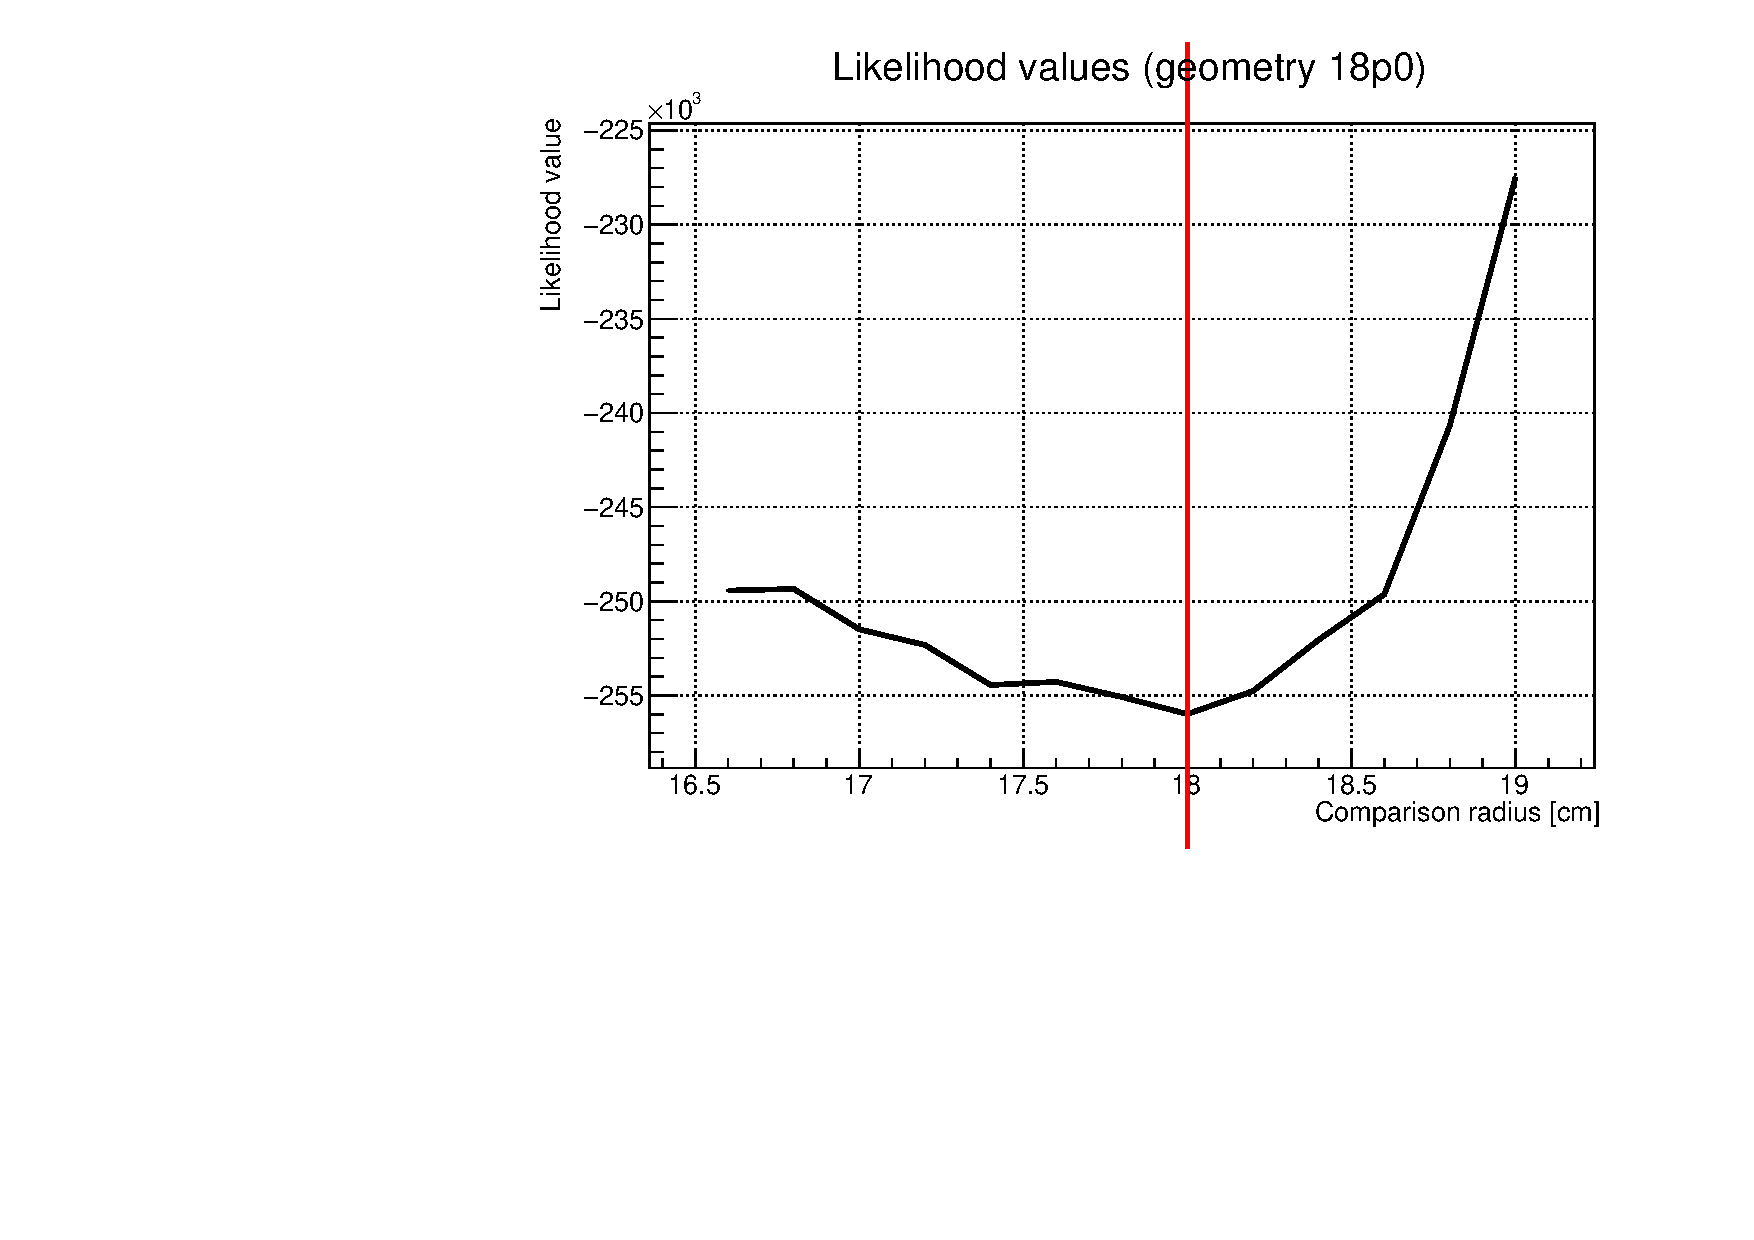
\includegraphics[width=4.2cm, height=3.2cm]{figs/likelihood250LowStat/likelihood18p0.pdf} 
\end{minipage} \vfill

In this case, it does seem that increasing the number of simulated events improve quite a lot the results (note that 10.000 events correspond to 1 minute of data taking only). \vfill
\end{frame}










%Conclusions
\begin{frame}{Conclusions}
\justifying
In conclusion, we developed a new framework allowing us to:
\begin{itemize}
\justifying
\item Quickly generate thousands of Monte-Carlo experiments for different pipe geometries without relying on Geant4
\item Compare the output measurement distributions expected at the bottom detector after propagating a muon through our Volume, using 	our own Propagator
\item Compute the likelihood of a given measurement with respect to different pipe geometries, in order to find a way to estimate the thickness of a steel pipe by studying the deviation of incident cosmic muons
\item And plot all the results obtained.
\end{itemize} \vfill

\begin{exampleblock}{}
\justifying
With this framework, we were able to determine the thickness of such pipes with \textbf{a precision of the order of the millimiter} by considering 10.000 events, which is equivalent to 1 minute of data taking only, therefore solving the initial problem solved. 
\end{exampleblock} \vfill

This exercise is only a first approach to the problem, and different improvements can be considered to \textbf{improve and/or generalize the results obtained}. \vfill
\end{frame}










%Back up
\begin{frame}{}
	\centering
	\huge{\textbf{\color{mycolor} Thank you  \color{black}}} \newline
	\LARGE{\textbf{\color{mycolor} for your attention! \color{black}}} \vfill
	\LARGE{\textbf{\color{mycolor} Backup slides \color{black}}}
\end{frame}

\appendix
	\backupbegin
	
\begin{frame}{Ionization}
\justifying
Ionization happens when the  incident muon gives some of its energy to the electrons of the absorber, as described by the Bethe-bloch formula. \vfill

\begin{equation*}
\label{eq:BB}
- \Bigl \langle \frac{dE}{dx} \Bigr \rangle = K z^2 \frac{Z}{A} \frac{1}{\beta^2} \left [\frac{1}{2} \ln \left (\frac{2 m_e c^2 \beta^2 \gamma^2 W_{\text{max}}}{I^2} - \beta^2 - \frac{\delta(\beta \gamma)}{2} \right ) \right ]
\end{equation*} \vfill

The \textbf{mass stopping power} of material depends on:
\begin{itemize}
	\item The charge number of incident particle $z$
	\item The atomic mass and charge of absorber $A$ and $Z$
	\item The relativistic factors $\beta$ and $\gamma$
	\item The maximum possible energy transfer to an electron in a single collision $W_{\text{max}}$
	\item And the mean excitation energy $I$.
\end{itemize} \vfill
\end{frame}

\begin{frame}{Ionization}
\justifying
Cosmic muons have an energy of the order of the GeV and are therefore referred to as minimum ionizing particles, so ionization is not considered in this work.
\begin{center}
	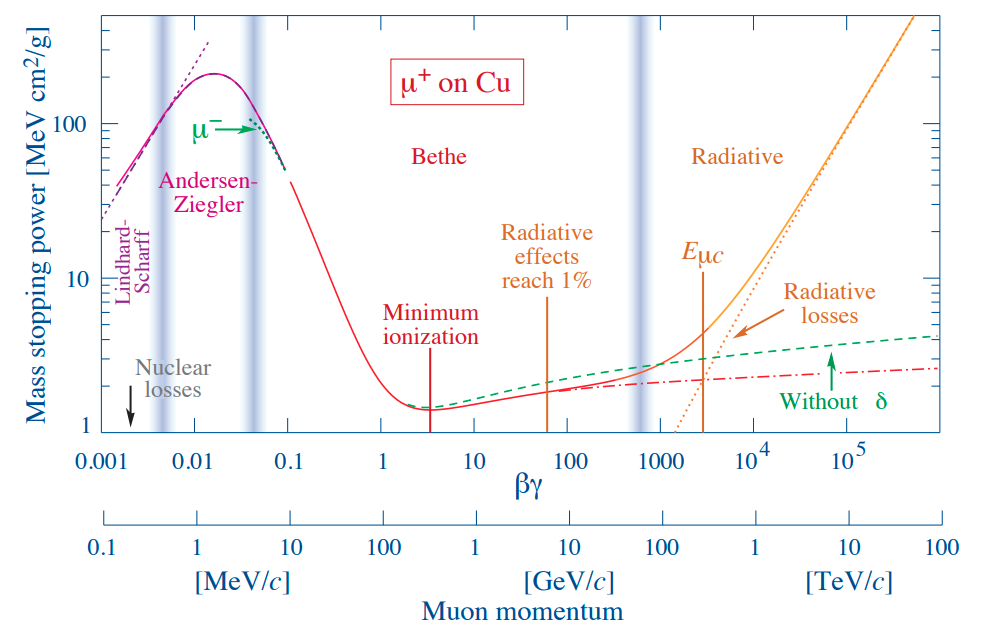
\includegraphics[width=10cm, height=6cm]{figs/BB.png}
	\end{center}
\end{frame}

\begin{frame}{Multiple Coulomb scattering}
\justifying
Inducing a \alert{\textbf{stochastic deviation}} whose central angular deviation can be described by a Gaussian of width $\theta_0$ under our experimental conditions.

\begin{equation*}
\label{eq:Moliere}
\theta_0 = \frac{13.6 \text{ MeV}}{\beta c p} z \sqrt{\frac{x}{X_0}} \left [1 + 0.038 \ln \left (\frac{x z^2}{X_0 \beta^2} \right ) \right ]
\end{equation*}

\begin{center}
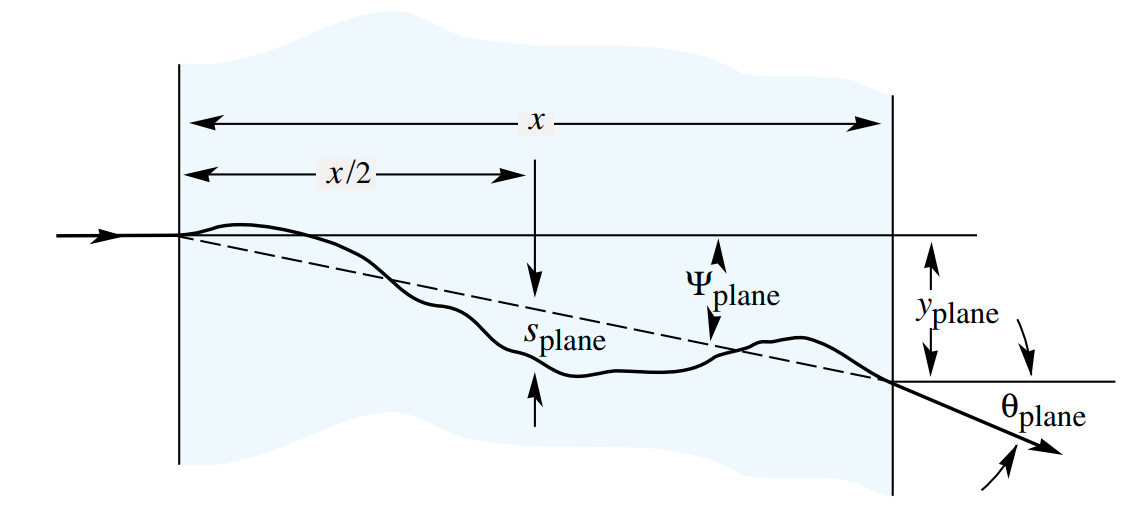
\includegraphics[width=8cm, height=3.5cm]{figs/moliere.png}
\end{center} \vfill

Highly correlated deviation parameters ($\rho_{\theta_\text{plane}, y_\text{plane}}=\sqrt{3}/2$). The pairs ($\theta_\text{plane}$, $y_\text{plane}$) are approximately distributed by a bi-dimensional Gaussian distribution with a given covariance:

\begin{equation}
\text{Cov}(\theta_\text{plane}, y_\text{plane}) = \begin{bmatrix}
\theta^2_0 & \frac{\theta_0^2x}{2} \\
\frac{\theta_0^2x}{2} & \frac{\theta_0^2x^2}{3} 
\end{bmatrix}
\end{equation} \vfill
\end{frame}

\begin{frame}{Muon detectors}
\justifying
\begin{minipage}[c]{.58\textwidth}
\justifying
Multiwire proportional chambers use an array of high-voltage wires, placed within a chamber filled with a gas, in which an electric field is created. \\ \vspace{10pt}
A muon crosses the detector leaves small electric charges behind, collected by the wires while leaving a signal. The combination of the signals on the different wires give us information regarding the muon.
\end{minipage} \hfill
\begin{minipage}[c]{.39\textwidth}
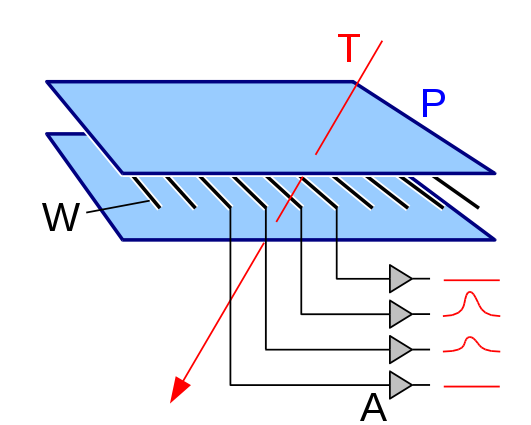
\includegraphics[width=4.2cm, height=3.5cm]{figs/wireChambers.png}
\end{minipage} \hfill \vfill

Most important parameters of a muon detector:
\begin{itemize}
\justifying
\item The \textbf{spatial resolution}, ideally as small as possible
\item The \textbf{acceptance}, related to the size of the detector
\item The \textbf{efficiency}, which should be high to make the measurement reliable and fast.
\end{itemize}
\end{frame}

\begin{frame}{Experimental setup}
\justifying
\begin{minipage}[c]{.50\textwidth}
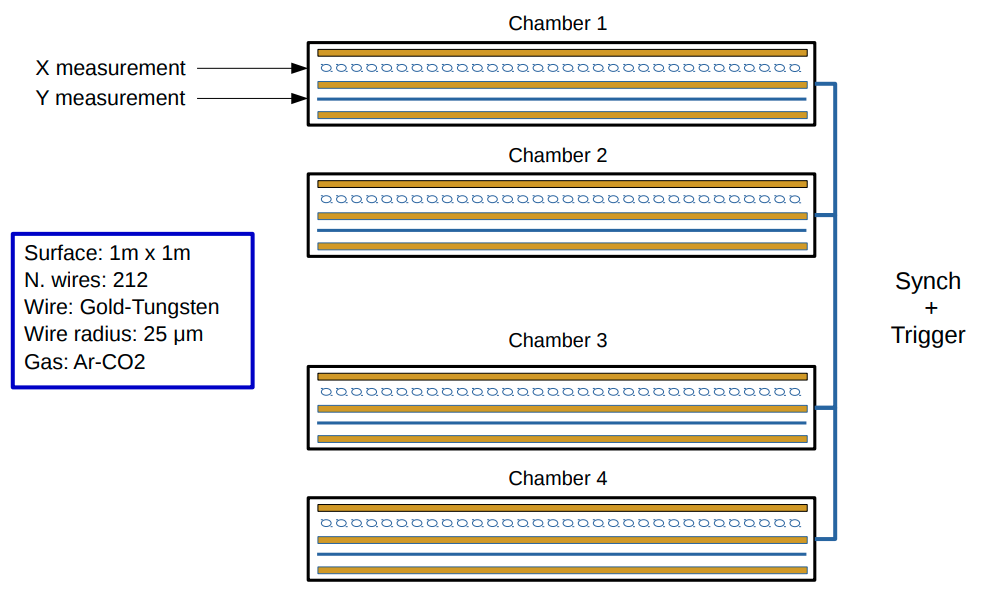
\includegraphics[width=5.5cm, height=3.7cm]{figs/muonChambers.png}
\end{minipage} \hfill
\begin{minipage}[c]{.49\textwidth}
\justifying
Quite simple experimental setup:
\begin{itemize}
\justifying
\item Two $1m^2$ detectors placed below and above the object under investigation
\item Two chambers in each detector, to measure the position and direction of muons along the x and y axes
\item Each chamber is filled with a mixture of Argon and CO$_2$
\item More than 200 wires separated by 4mm make up each chamber
\end{itemize}
\end{minipage} \hfill  \vfill

The data is collected from a USB stick and goes through a complete \textbf{\alert{reconstruction process}} before being available in a rootfile, as detailed in the backup. \vfill
\end{frame}

\begin{frame}{Data flow}
\begin{center}
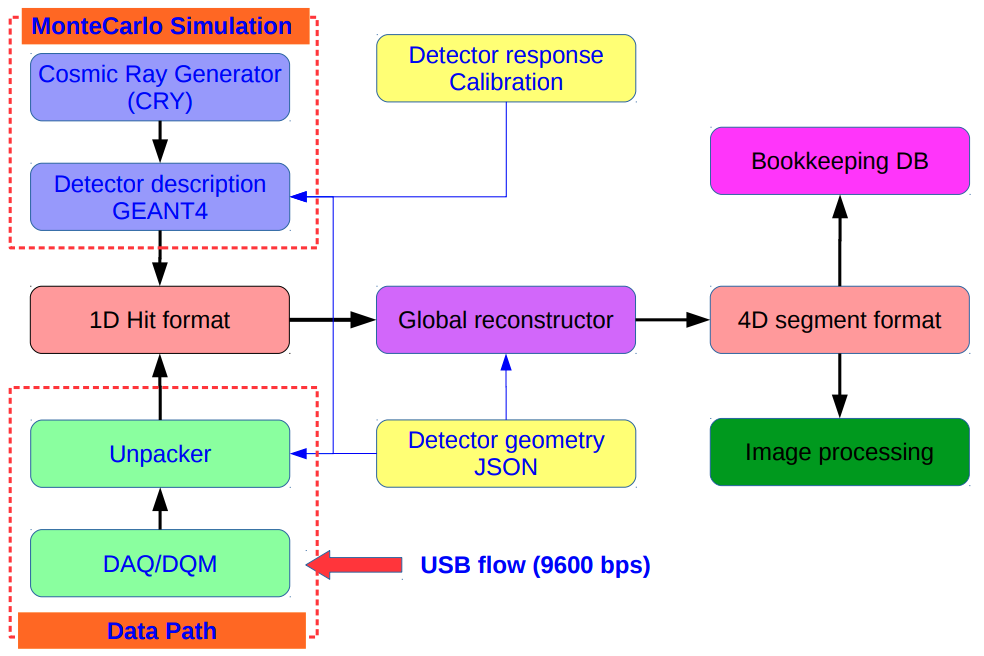
\includegraphics[width=7.5cm, height=6cm]{figs/dataFlow.png}
\end{center}
\end{frame}

\begin{frame}{Positional and angular deviation parameters}
\justifying
Main parameters used throughout this work:

\begin{equation*}
\label{eq:deviationPos}
\begin{dcases}
\Delta \text{x} = x_2 + d (v_{x2} - x_1)  \\
\Delta \text{y} = y_2 + d (v_{y2} - y_1)
\end{dcases}
\end{equation*}

\begin{equation*}
\label{eq:deviationDir}
\begin{dcases}
\Delta \theta_x = \arctan \left ({\frac{v_{x2}}{v_{z2}}} \right ) - \arctan \left ({\frac{v_{x1}}{v_{z1}}} \right ) \\
\Delta \theta_y = \arctan \left ({\frac{v_{y2}}{v_{z2}}} \right ) - \arctan \left ({\frac{v_{y1}}{v_{z1}}} \right )
\end{dcases}
\end{equation*} \vfill

Bi-dimensional histograms ($\Delta$x vs $\Delta \theta_x$ and $\Delta$y vs $\Delta \theta_y$) are filled with these values, smoothened and used for the computation of the likelihood. \vfill
\end{frame}

%\begin{frame}{Generator}
%\justifying
%The Generator is a C++ set of functions, built in order to generate Monte-Carlo simulations reproducing the actual experiment for a given geometry and to avoid relying too much on Geant4, which is quite slow. \vfill
%
%Pre-generated CRY information is then read and simply propagated through the Volume considered, using our PipeReconstructor, in order to simulate such experiments. \vfill
%\end{frame}

\begin{frame}{Generator validation}

\vspace{-5pt}
\begin{minipage}[c]{.32\textwidth}
\begin{exampleblock}{} \begin{center}Bottom X position\end{center} \end{exampleblock}
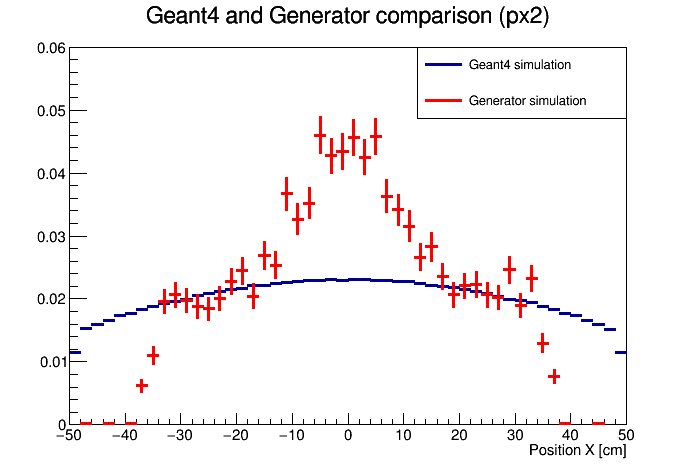
\includegraphics[width=4.2cm, height=3.2cm]{figs/px2-17p2vs17p2.png} 
\end{minipage}
\begin{minipage}[c]{.32\textwidth}
\begin{exampleblock}{} \begin{center}$\Delta_x$ parameter\end{center} \end{exampleblock}
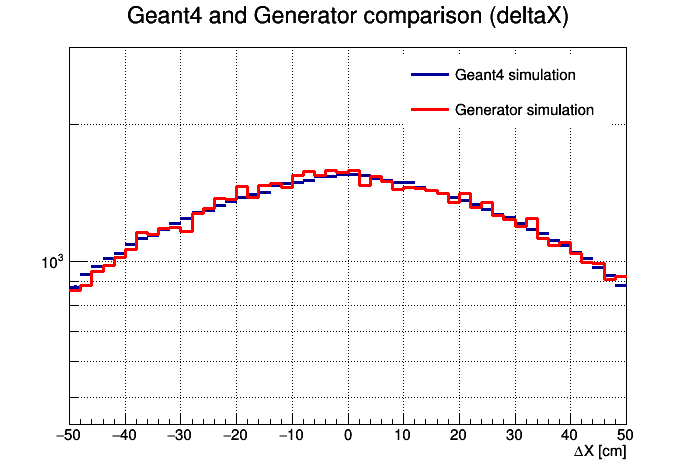
\includegraphics[width=4.2cm, height=3.2cm]{figs/deltaX-17p2vs17p2.png}
\end{minipage}
\begin{minipage}[c]{.32\textwidth}
\begin{exampleblock}{} \begin{center}$\Delta \theta_x$ parameter\end{center} \end{exampleblock}
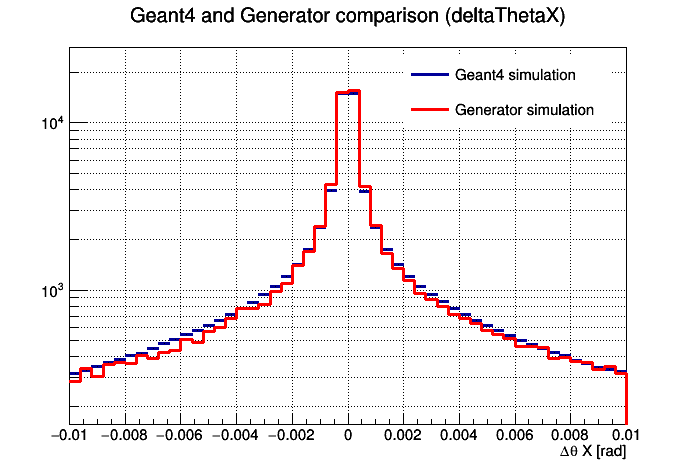
\includegraphics[width=4.2cm, height=3.2cm]{figs/deltaThetaX-17p2vs17p2.png}
\end{minipage} \vspace{-8pt}

\begin{minipage}[c]{.32\textwidth}
\begin{exampleblock}{} \begin{center}Bottom Y position\end{center} \end{exampleblock}
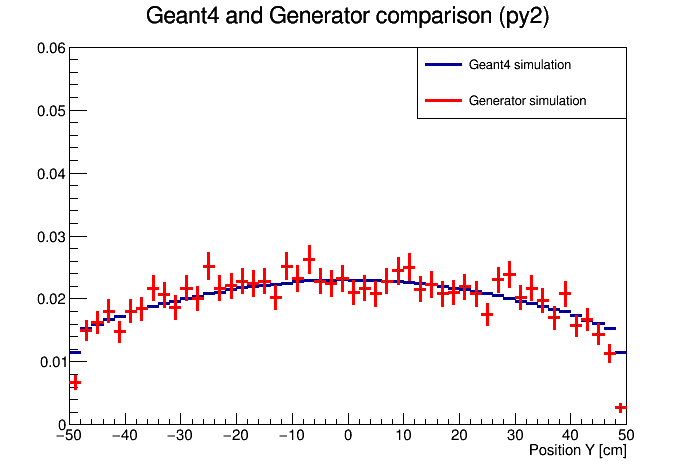
\includegraphics[width=4.2cm, height=3.2cm]{figs/py2-17p2vs17p2.png} 
\end{minipage}
\begin{minipage}[c]{.32\textwidth}
\begin{exampleblock}{} \begin{center}$\Delta_y$ parameter\end{center} \end{exampleblock}
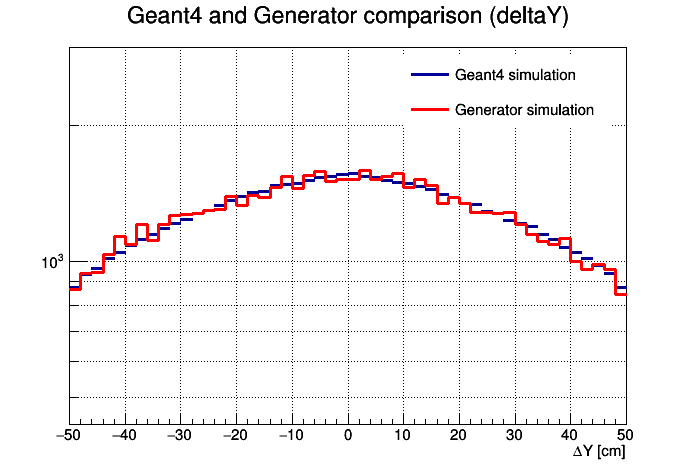
\includegraphics[width=4.2cm, height=3.2cm]{figs/deltaY-17p2vs17p2.png}
\end{minipage}
\begin{minipage}[c]{.32\textwidth}
\begin{exampleblock}{} \begin{center}$\Delta \theta_y$ parameter\end{center} \end{exampleblock}
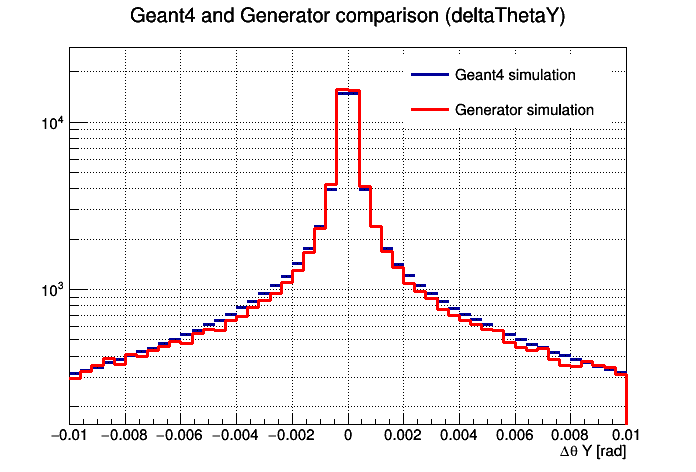
\includegraphics[width=4.2cm, height=3.2cm]{figs/deltaThetaY-17p2vs17p2.png}
\end{minipage} \vfill
\end{frame}

\begin{frame}{Pipes geometries}
The same comparison has been performed along the Y-axis. \vfill

\begin{figure}[htbp]
\centering
\begin{minipage}[b]{.49\textwidth}
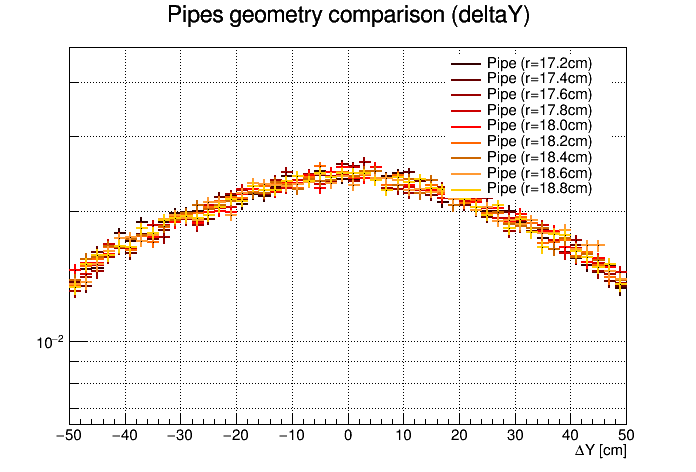
\includegraphics[width=6cm, height=4.8cm]{figs/deltaY.png}
\end{minipage}\hfill
\begin{minipage}[b]{.49\textwidth}
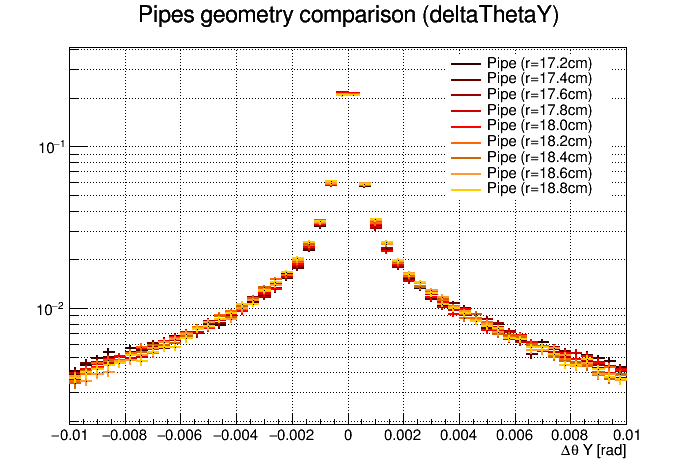
\includegraphics[width=6cm, height=4.8cm]{figs/deltaThetaY.png}
\end{minipage}\hfill
\end{figure} \vfill
\end{frame}

\begin{frame}{Likelihood curves (10.000 events, 100 iterations)}
\justifying
\begin{minipage}[c]{.32\textwidth}
\begin{exampleblock}{} \begin{center}$r = 16.8$cm\end{center} \end{exampleblock}
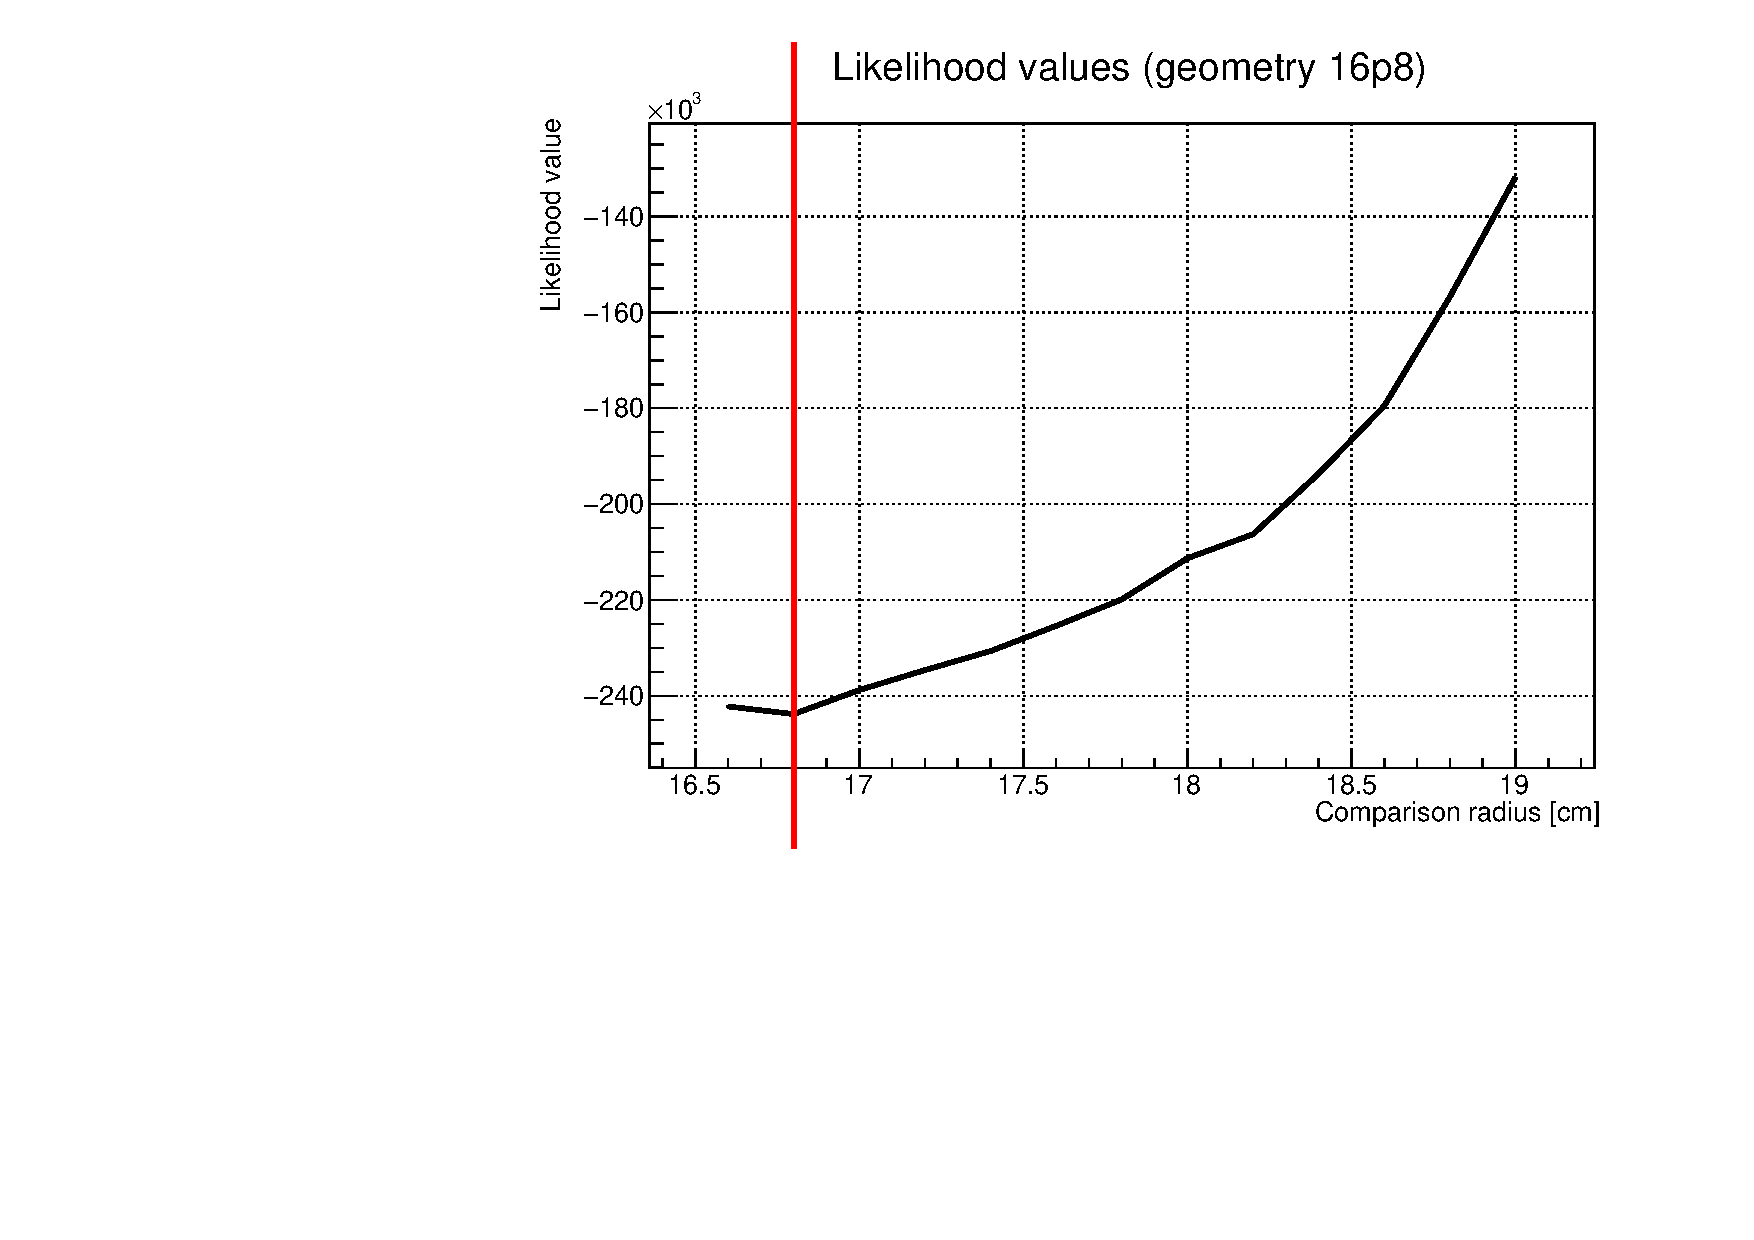
\includegraphics[width=4.2cm, height=3.2cm]{figs/likelihood100LowStat/likelihood16p8.pdf} 
\end{minipage}
\begin{minipage}[c]{.32\textwidth}
\begin{exampleblock}{} \begin{center}$r = 17.0$cm\end{center} \end{exampleblock}
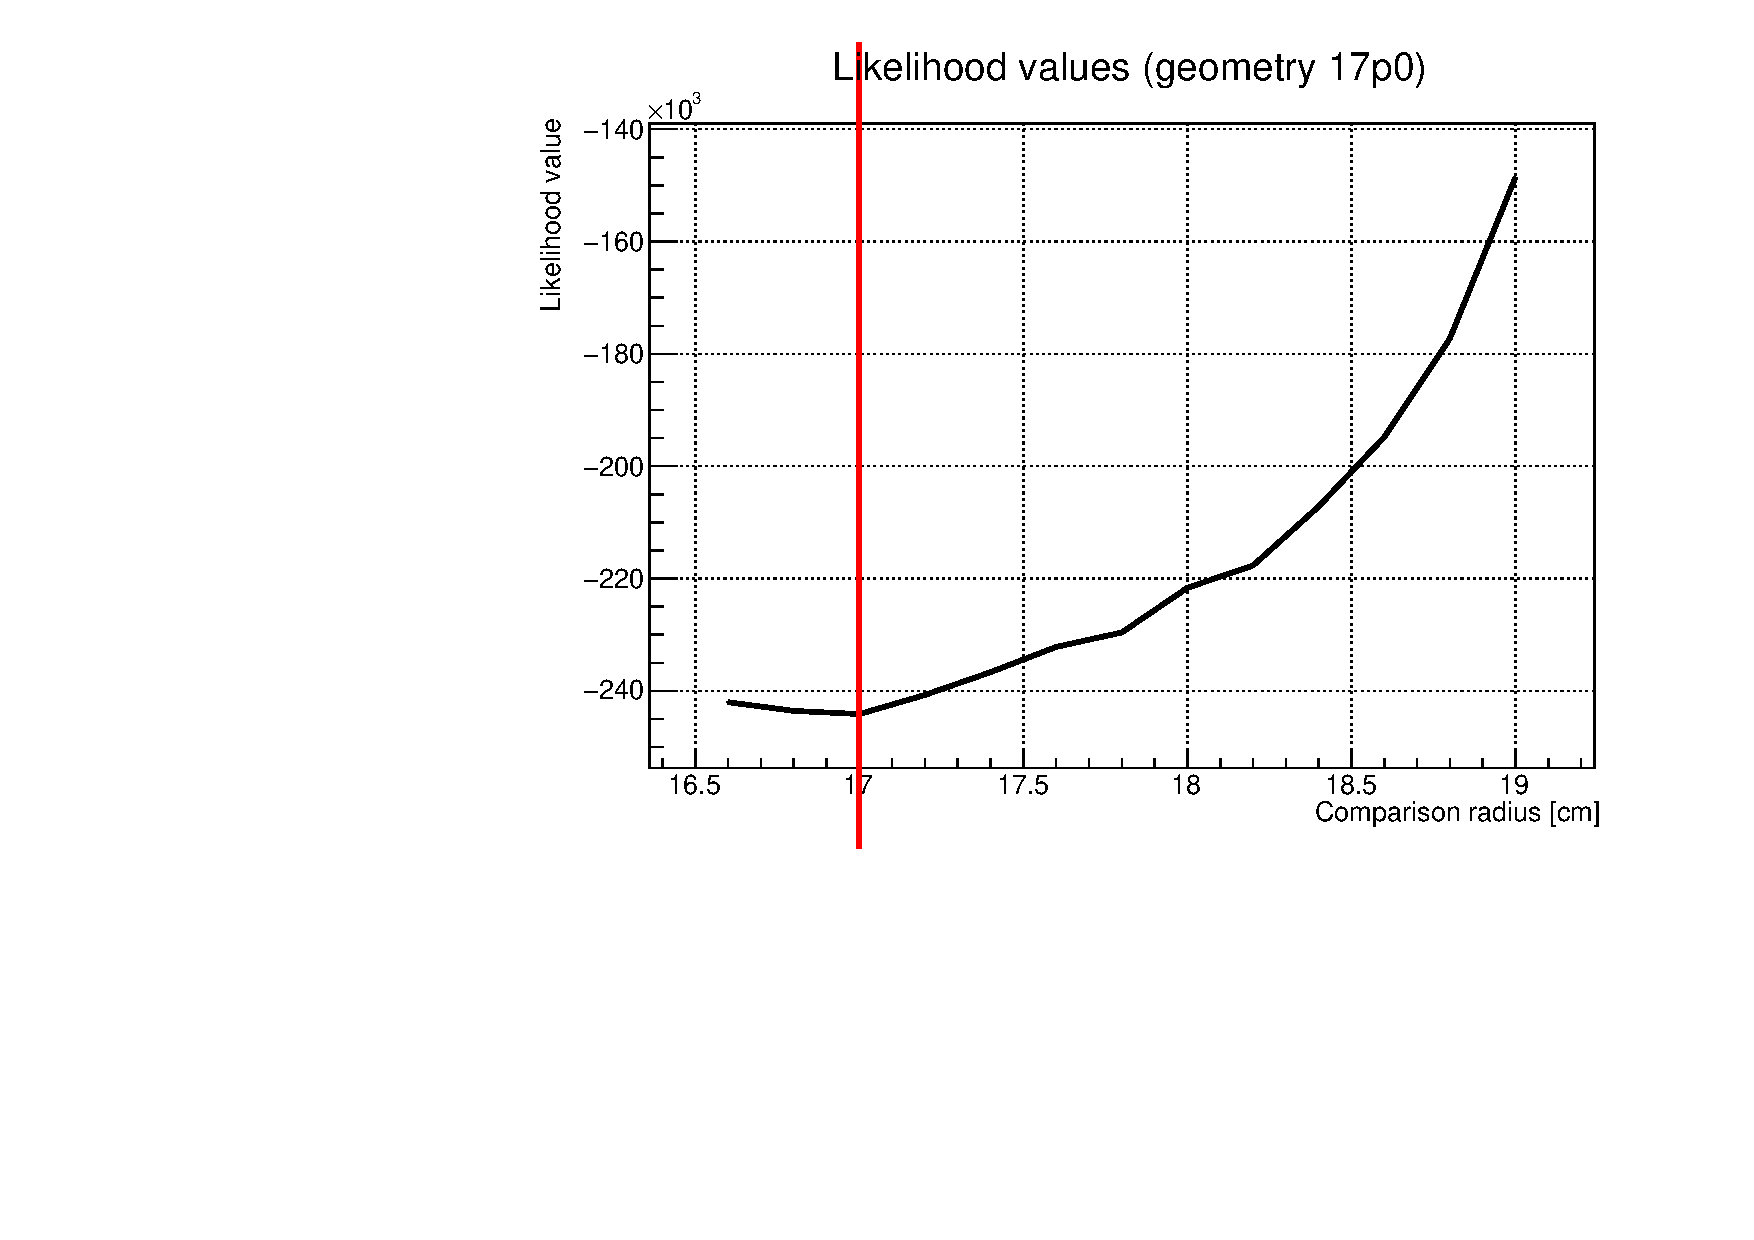
\includegraphics[width=4.2cm, height=3.2cm]{figs/likelihood100LowStat/likelihood17p0.pdf} 
\end{minipage}
\begin{minipage}[c]{.32\textwidth}
\begin{exampleblock}{} \begin{center}$r = 17.2$cm\end{center} \end{exampleblock}
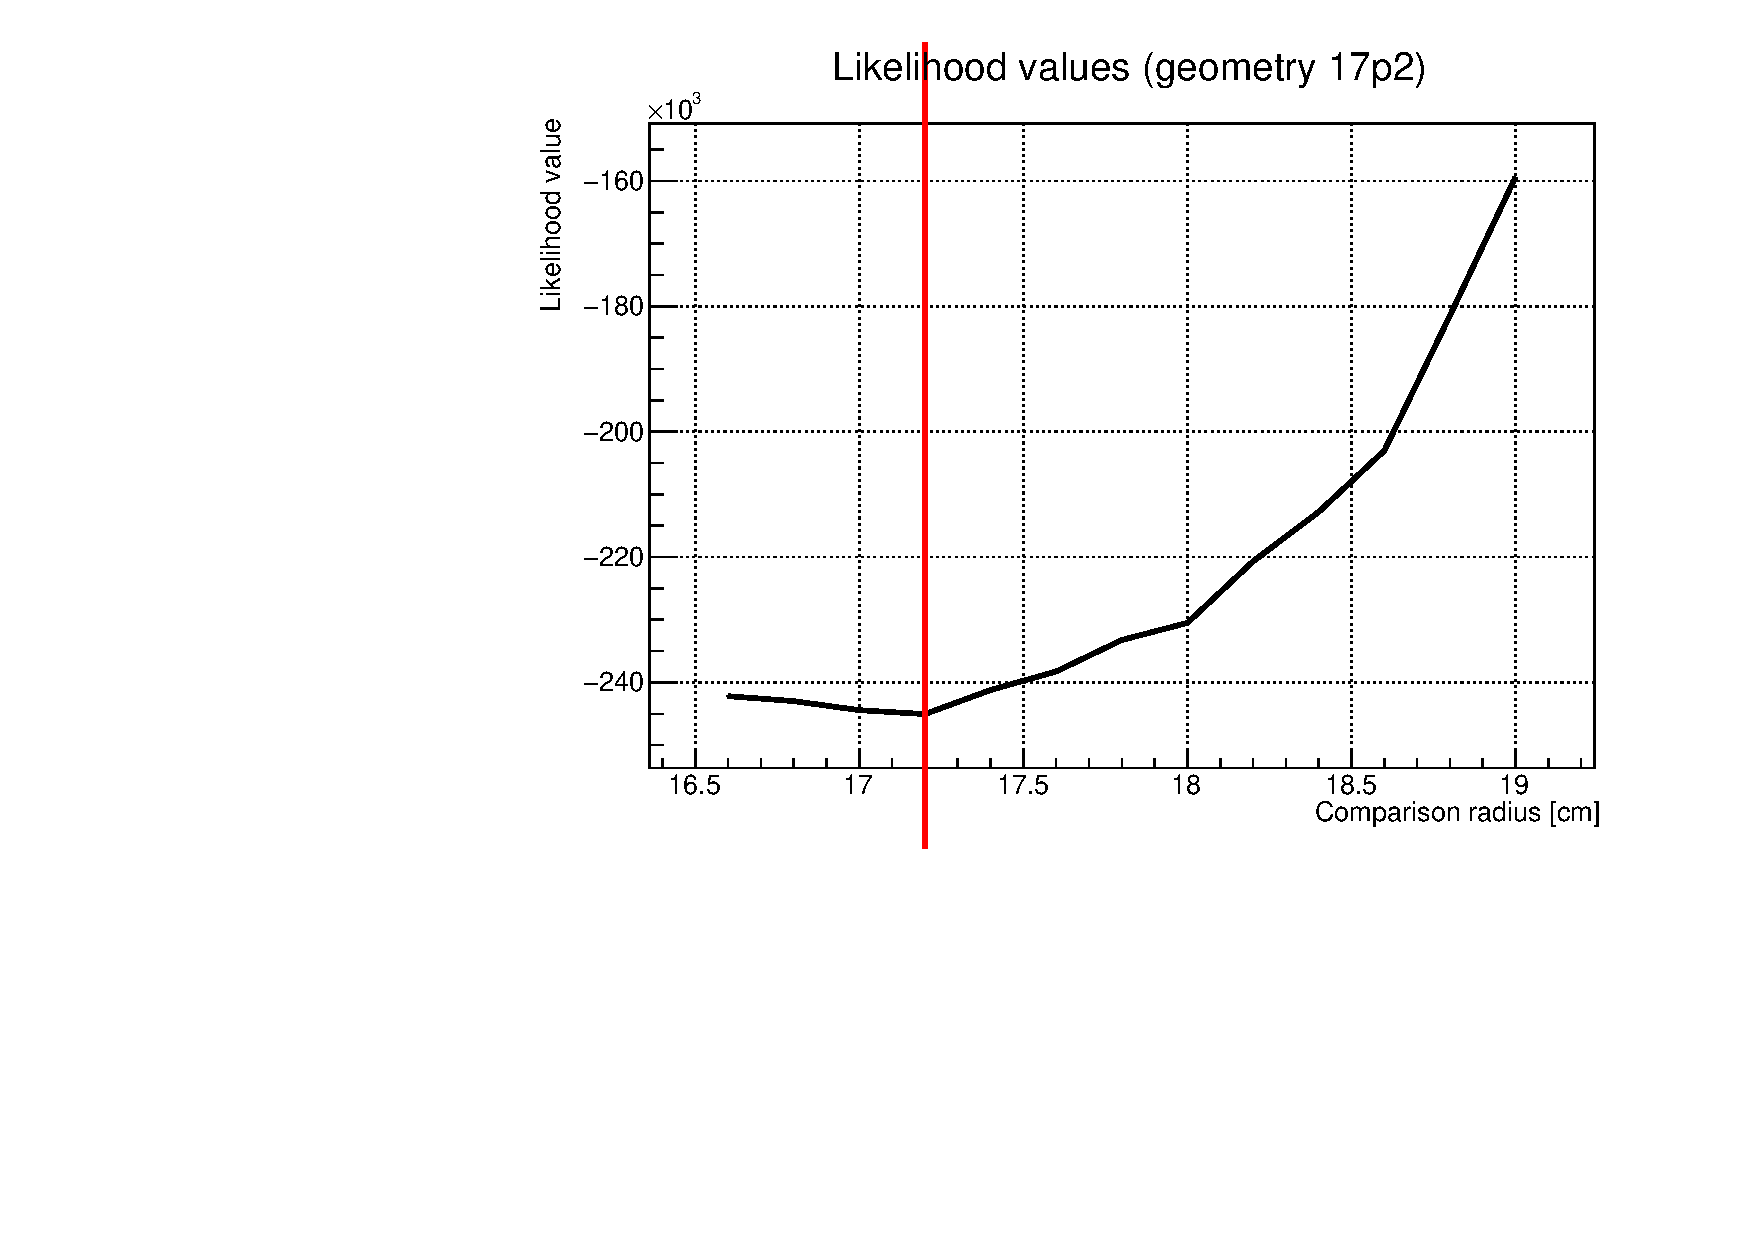
\includegraphics[width=4.2cm, height=3.2cm]{figs/likelihood100LowStat/likelihood17p2.pdf} 
\end{minipage}

\vspace{-5pt}
\begin{minipage}[c]{.32\textwidth}
\begin{exampleblock}{} \begin{center}$r = 17.4$cm\end{center} \end{exampleblock}
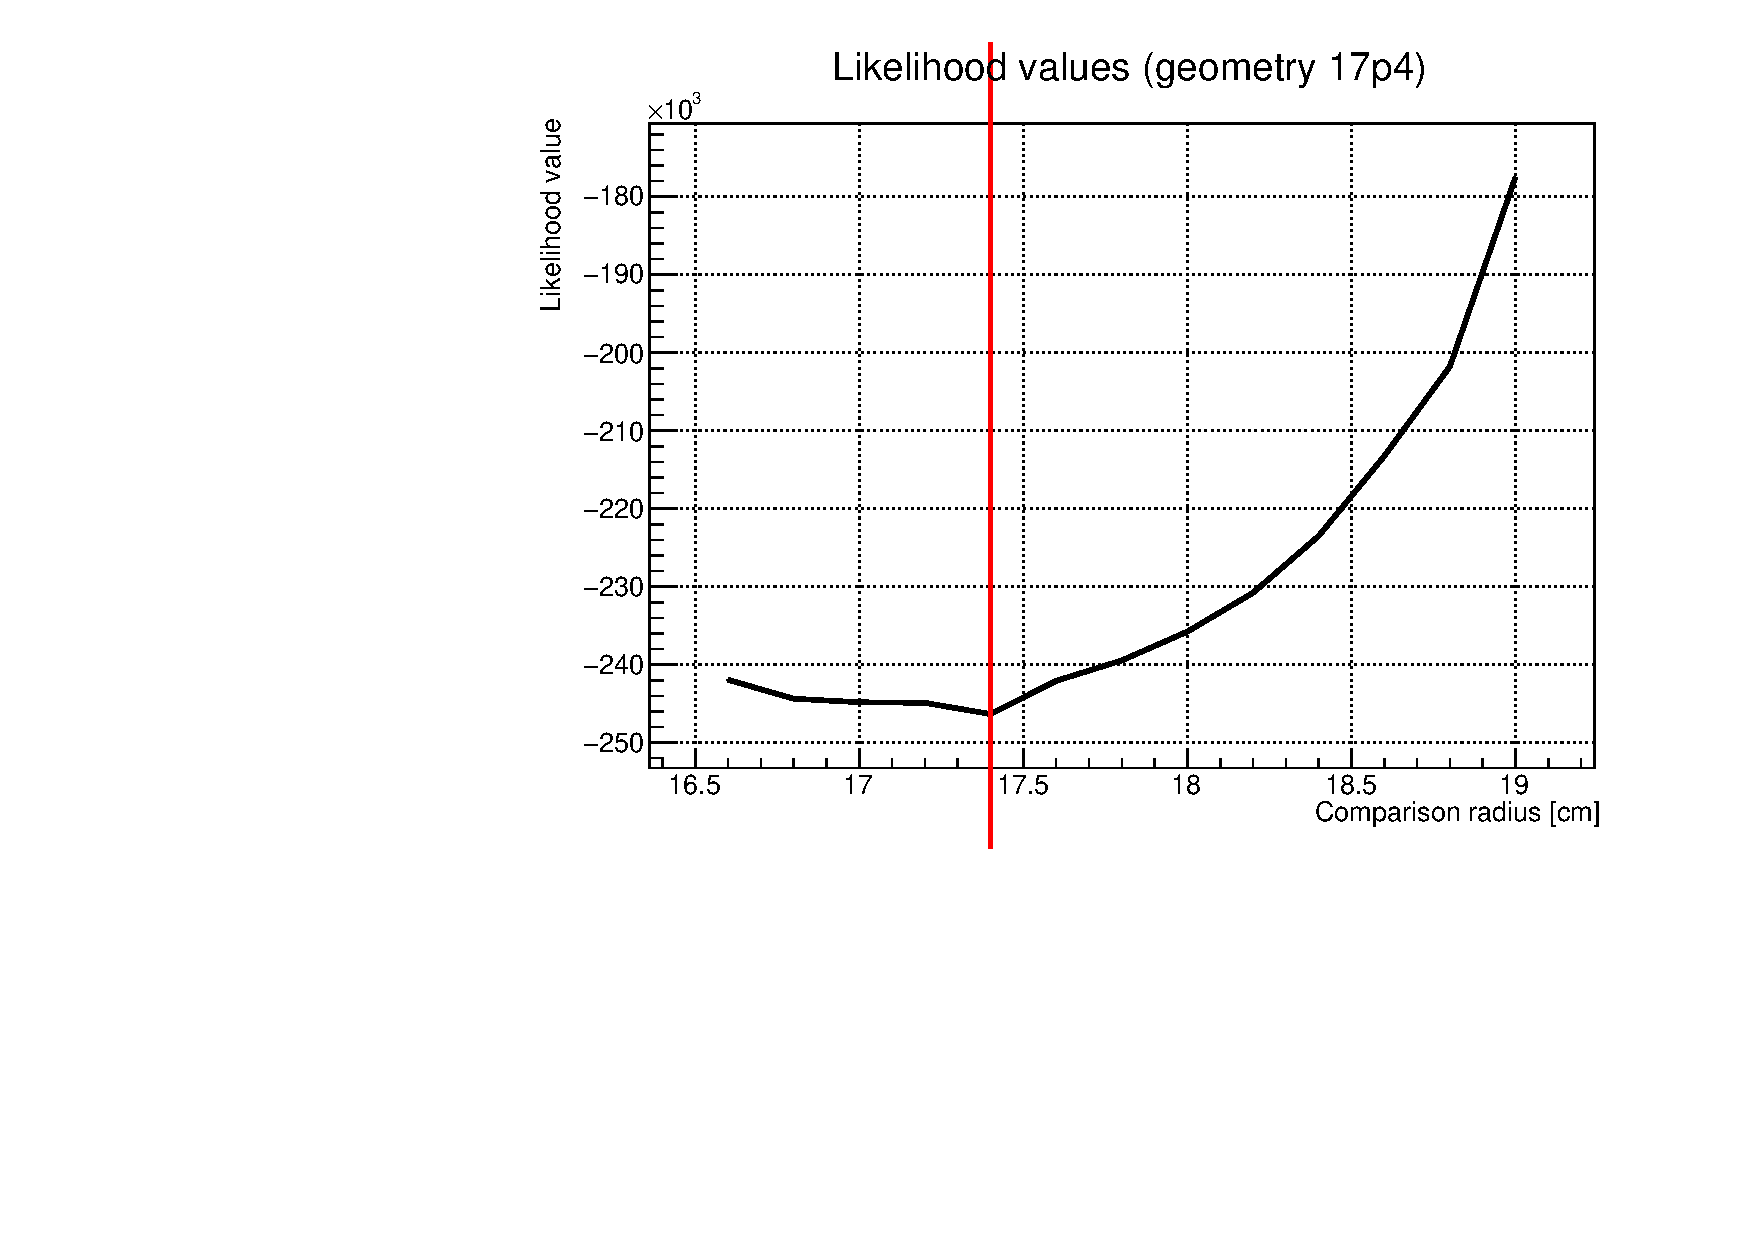
\includegraphics[width=4.2cm, height=3.2cm]{figs/likelihood100LowStat/likelihood17p4.pdf} 
\end{minipage}
\begin{minipage}[c]{.32\textwidth}
\begin{exampleblock}{} \begin{center}$r = 17.6$cm\end{center} \end{exampleblock}
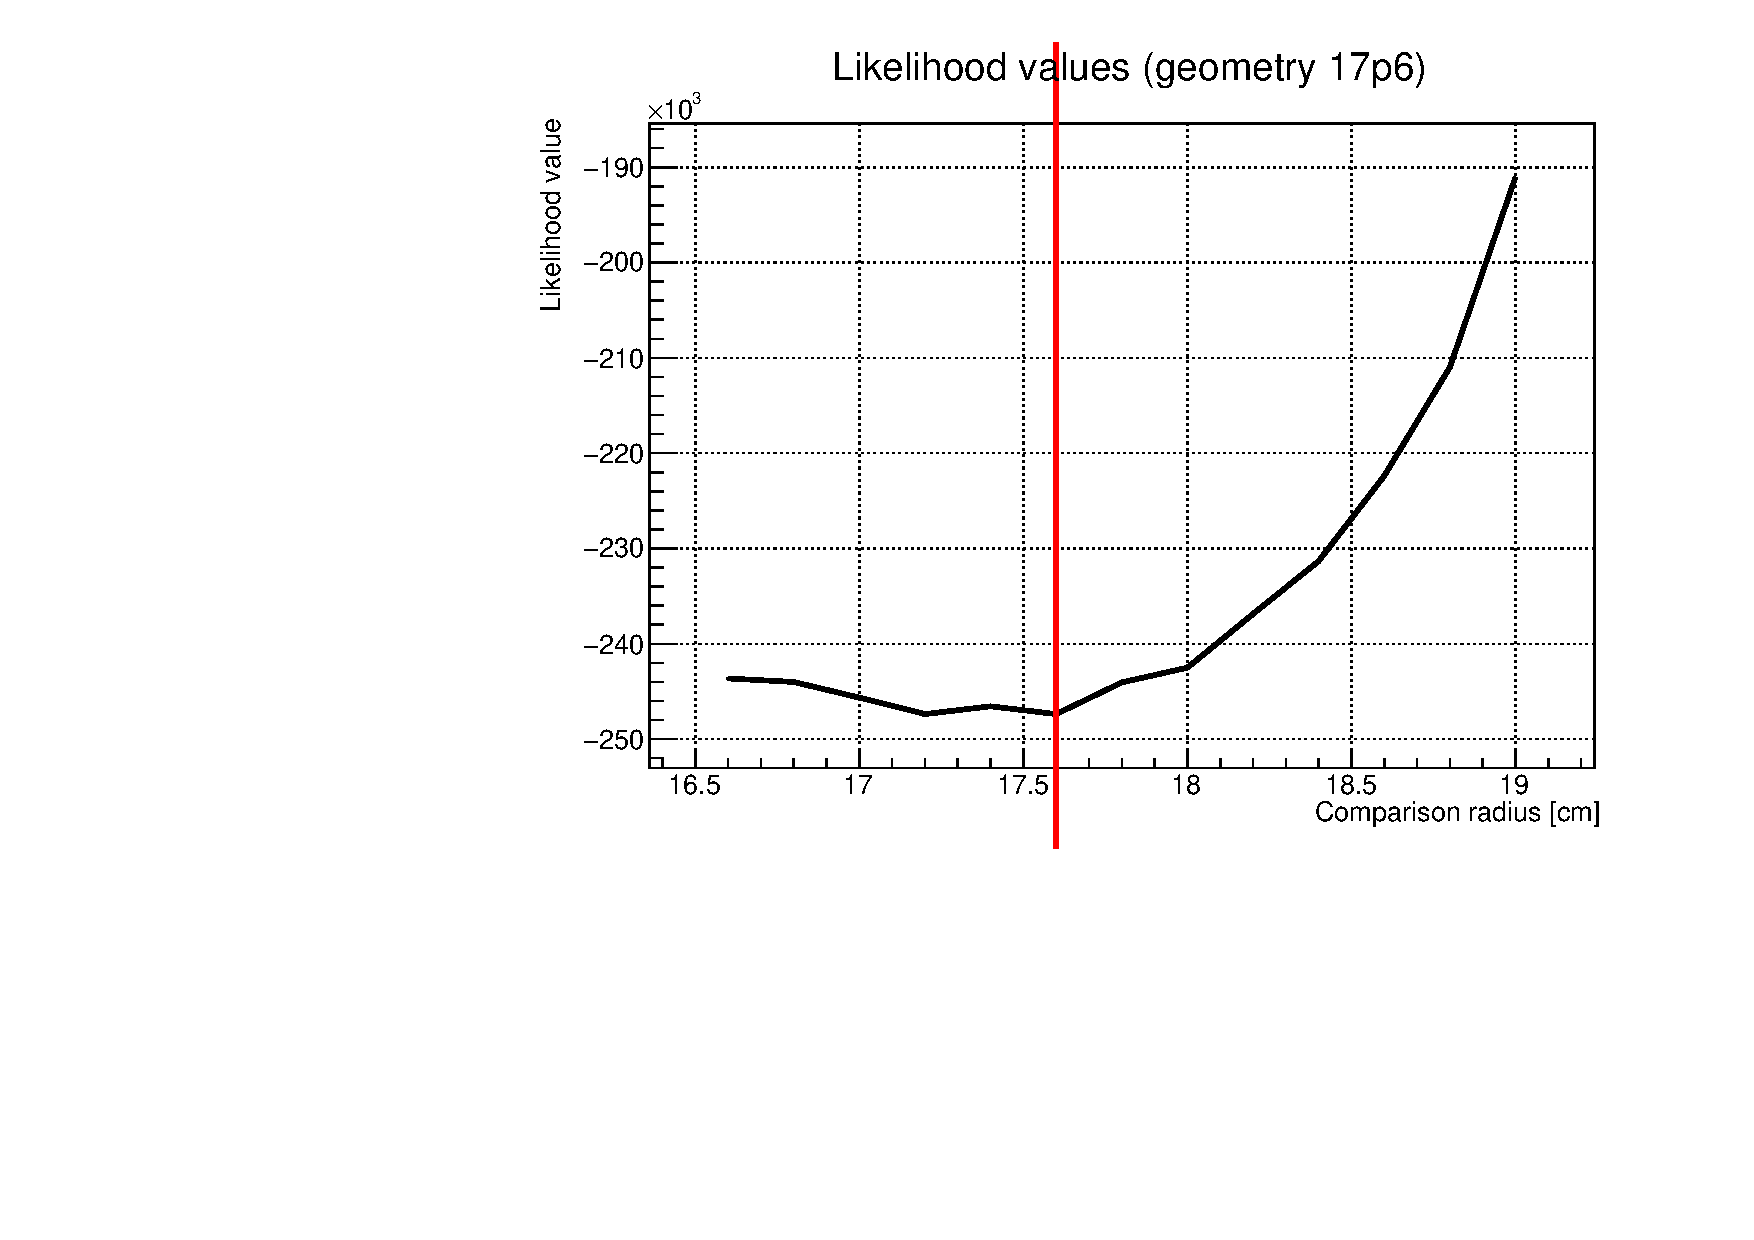
\includegraphics[width=4.2cm, height=3.2cm]{figs/likelihood100LowStat/likelihood17p6.pdf} 
\end{minipage}
\begin{minipage}[c]{.32\textwidth}
\begin{exampleblock}{} \begin{center}$r = 17.8$cm\end{center} \end{exampleblock}
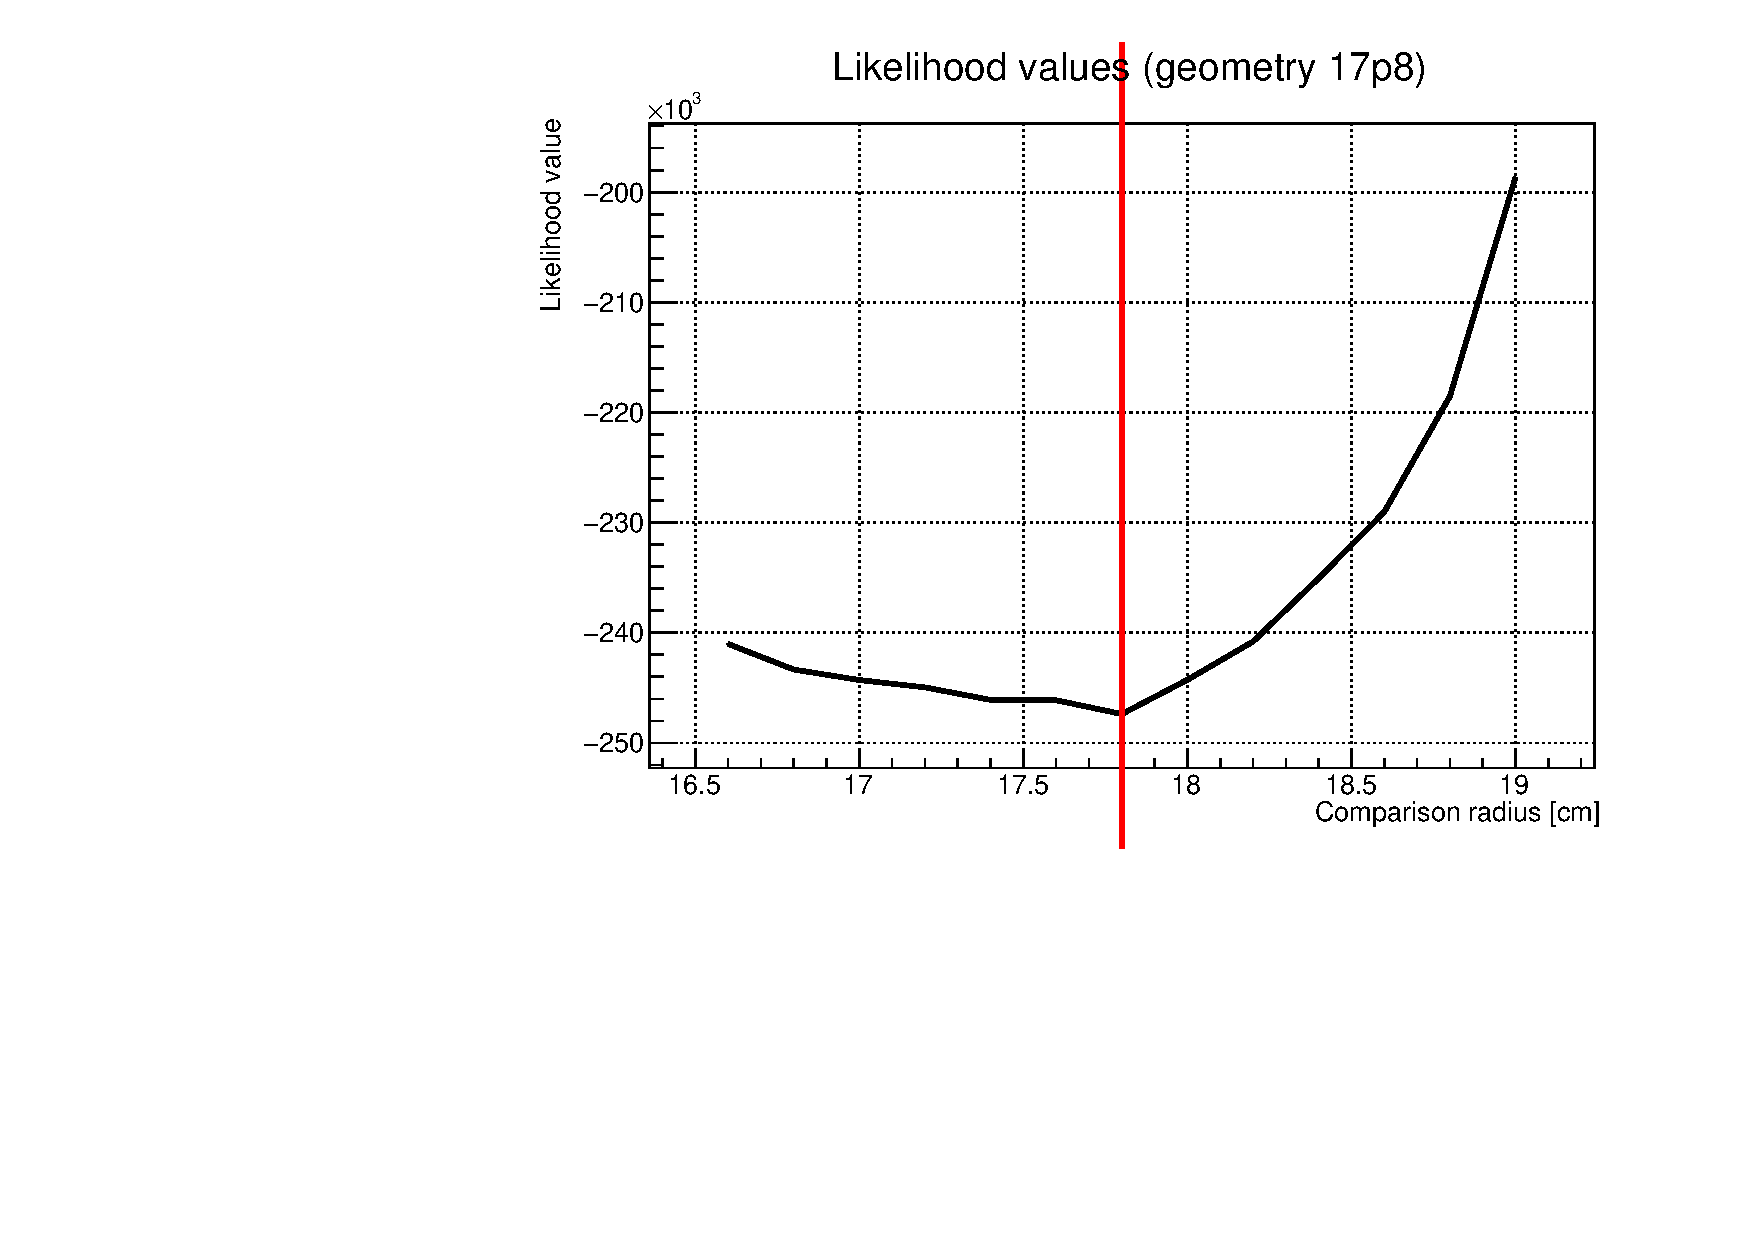
\includegraphics[width=4.2cm, height=3.2cm]{figs/likelihood100LowStat/likelihood17p8.pdf} 
\end{minipage}
\end{frame}

\begin{frame}{Likelihood curves (10.000 events, 100 iterations)}
\justifying
\begin{minipage}[c]{.32\textwidth}
\begin{exampleblock}{} \begin{center}$r = 18.0$cm\end{center} \end{exampleblock}
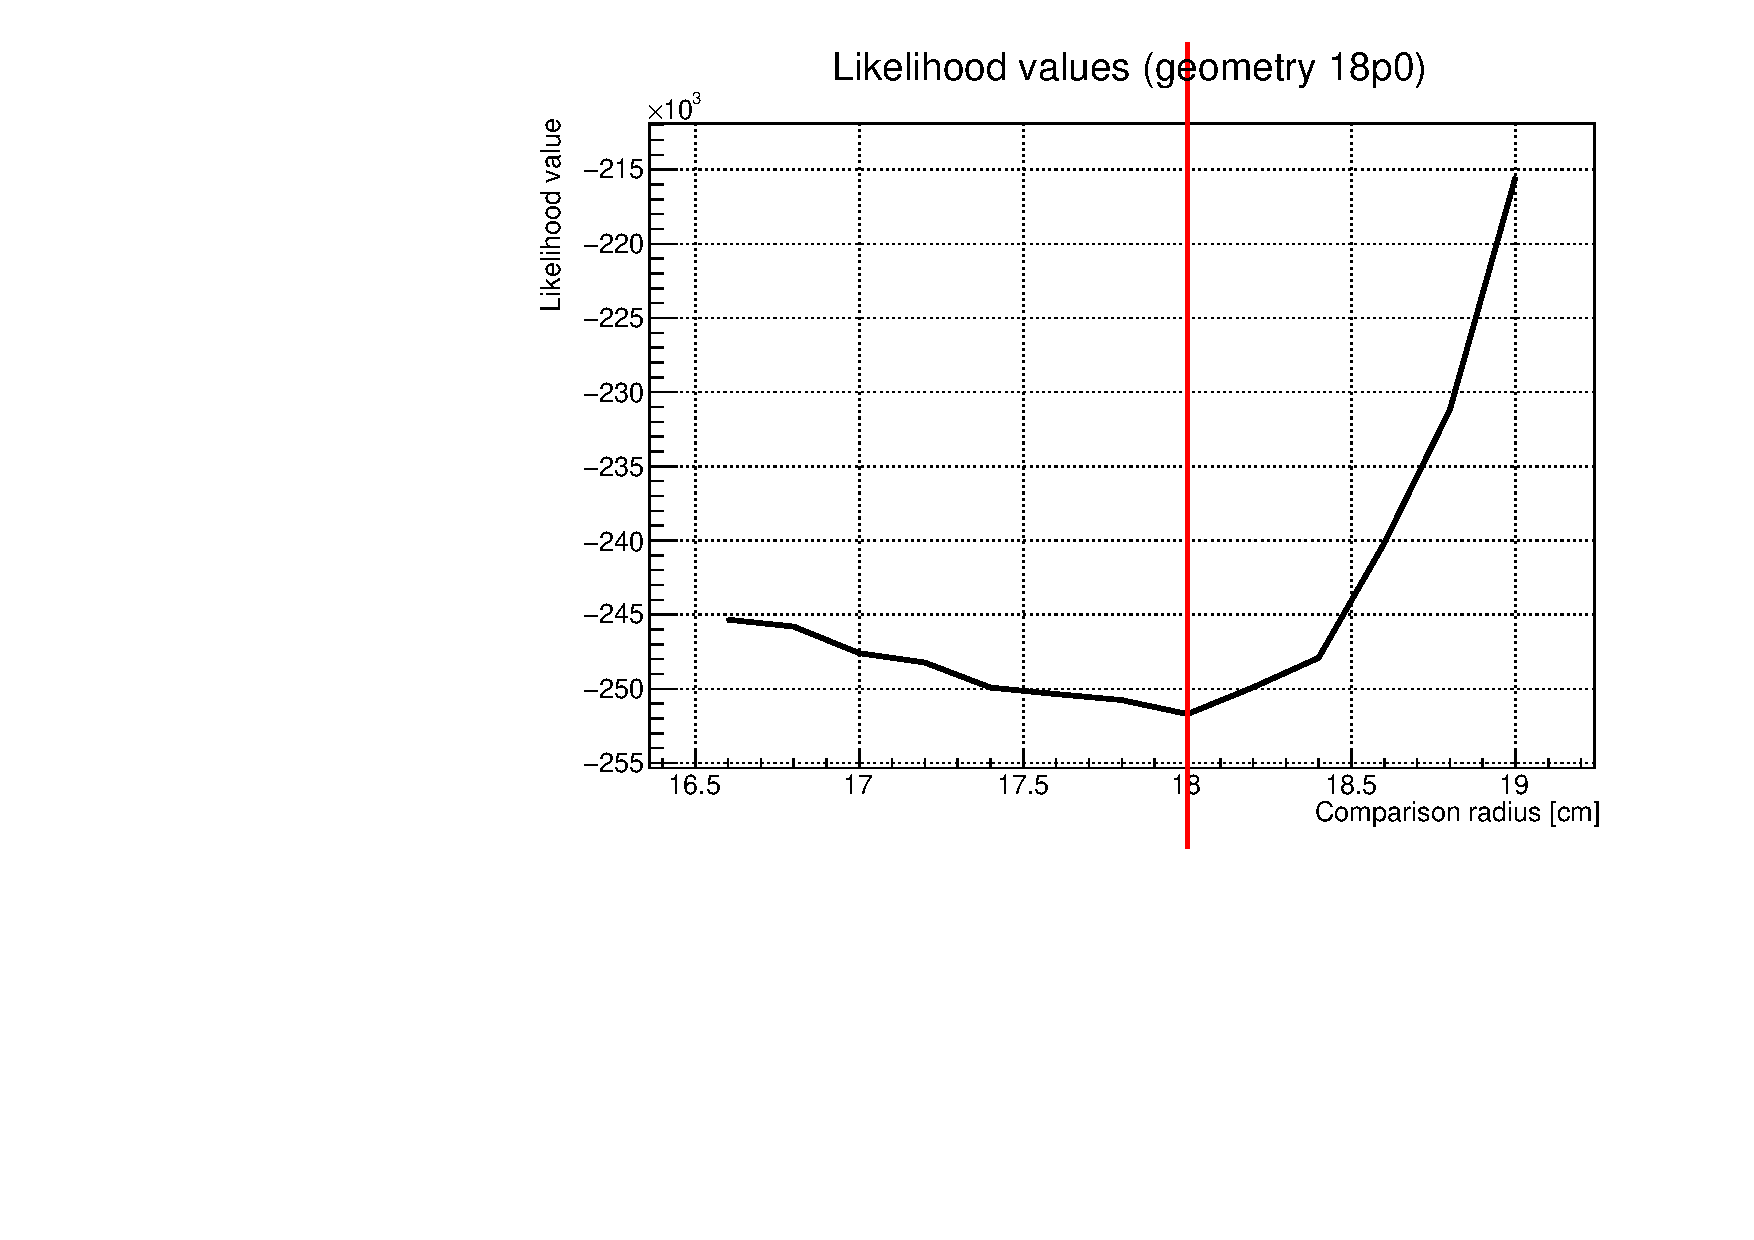
\includegraphics[width=4.2cm, height=3.2cm]{figs/likelihood100LowStat/likelihood18p0.pdf} 
\end{minipage}
\begin{minipage}[c]{.32\textwidth}
\begin{exampleblock}{} \begin{center}$r = 18.2$cm\end{center} \end{exampleblock}
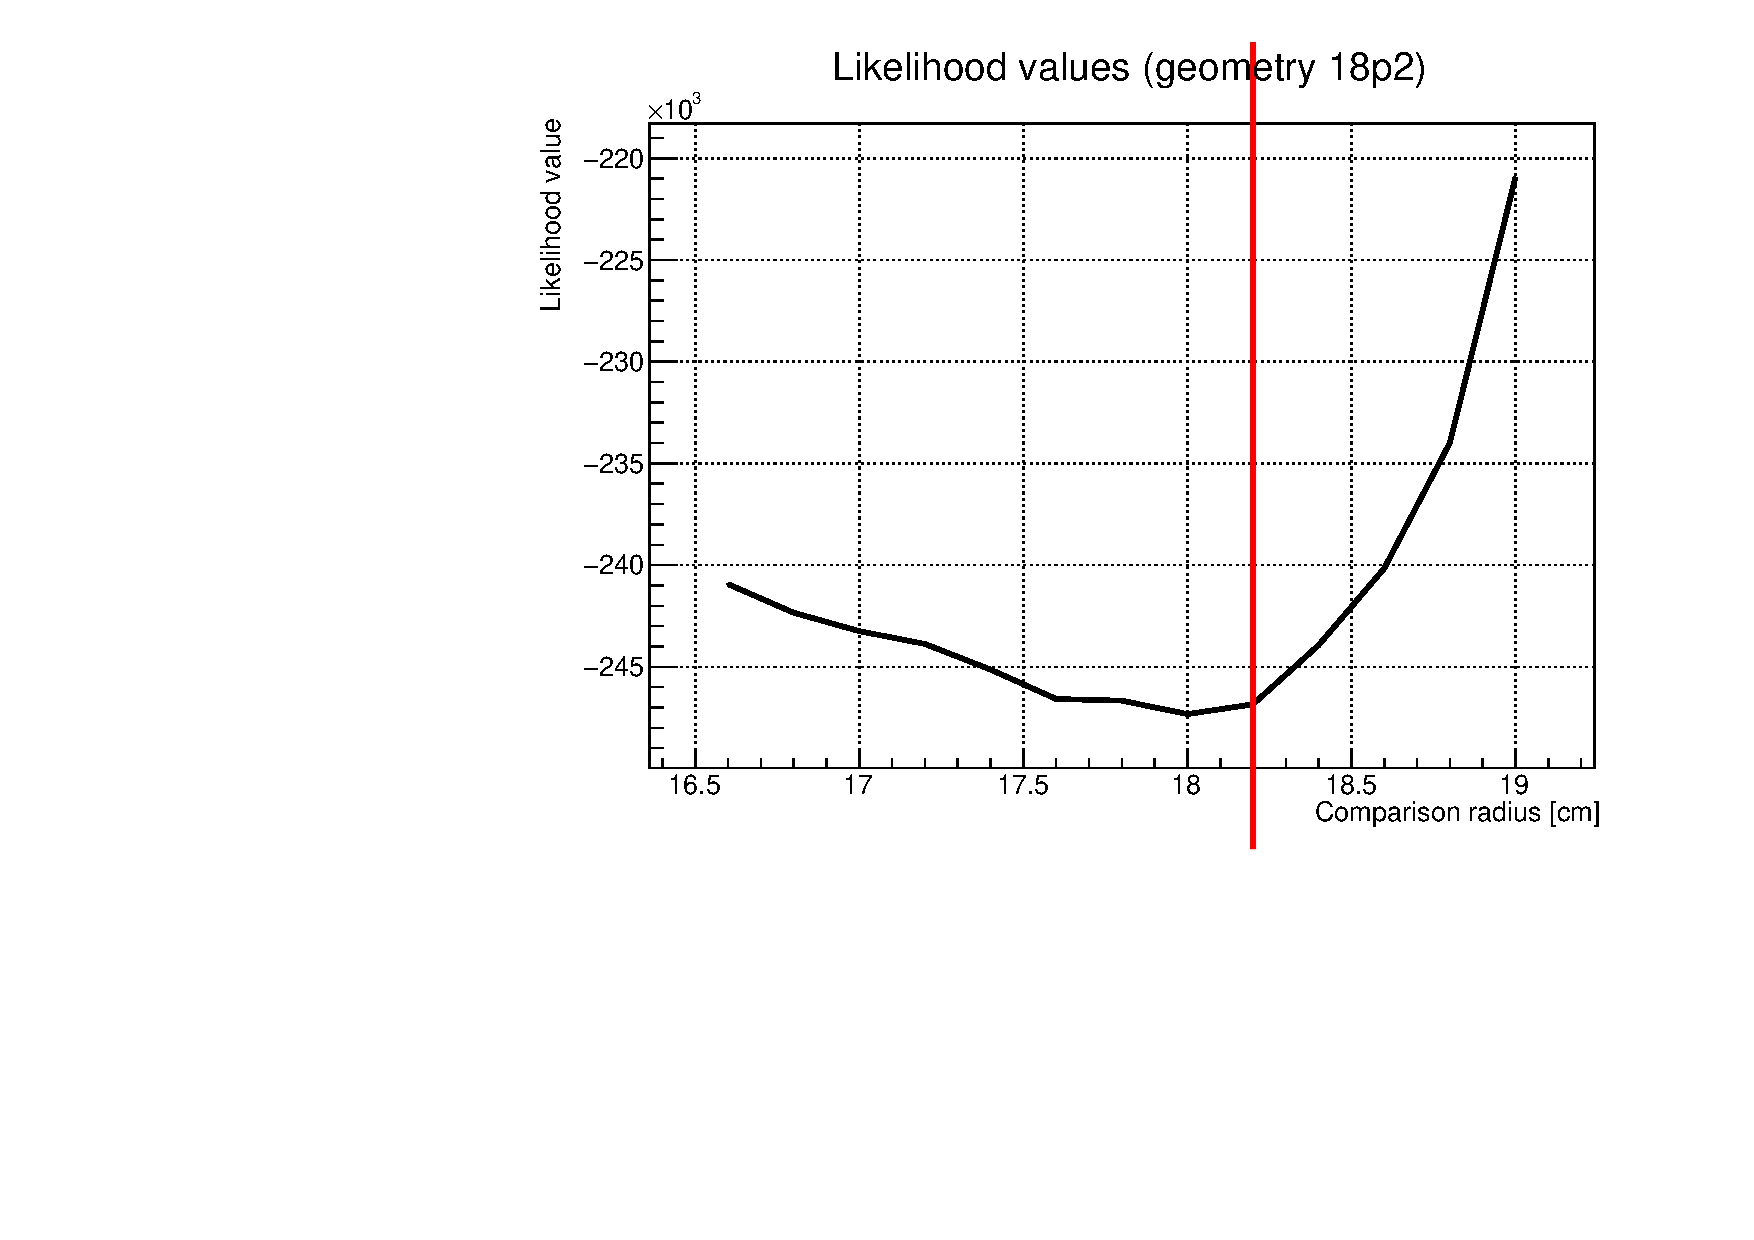
\includegraphics[width=4.2cm, height=3.2cm]{figs/likelihood100LowStat/likelihood18p2.pdf} 
\end{minipage}
\begin{minipage}[c]{.32\textwidth}
\begin{exampleblock}{} \begin{center}$r = 18.4$cm\end{center} \end{exampleblock}
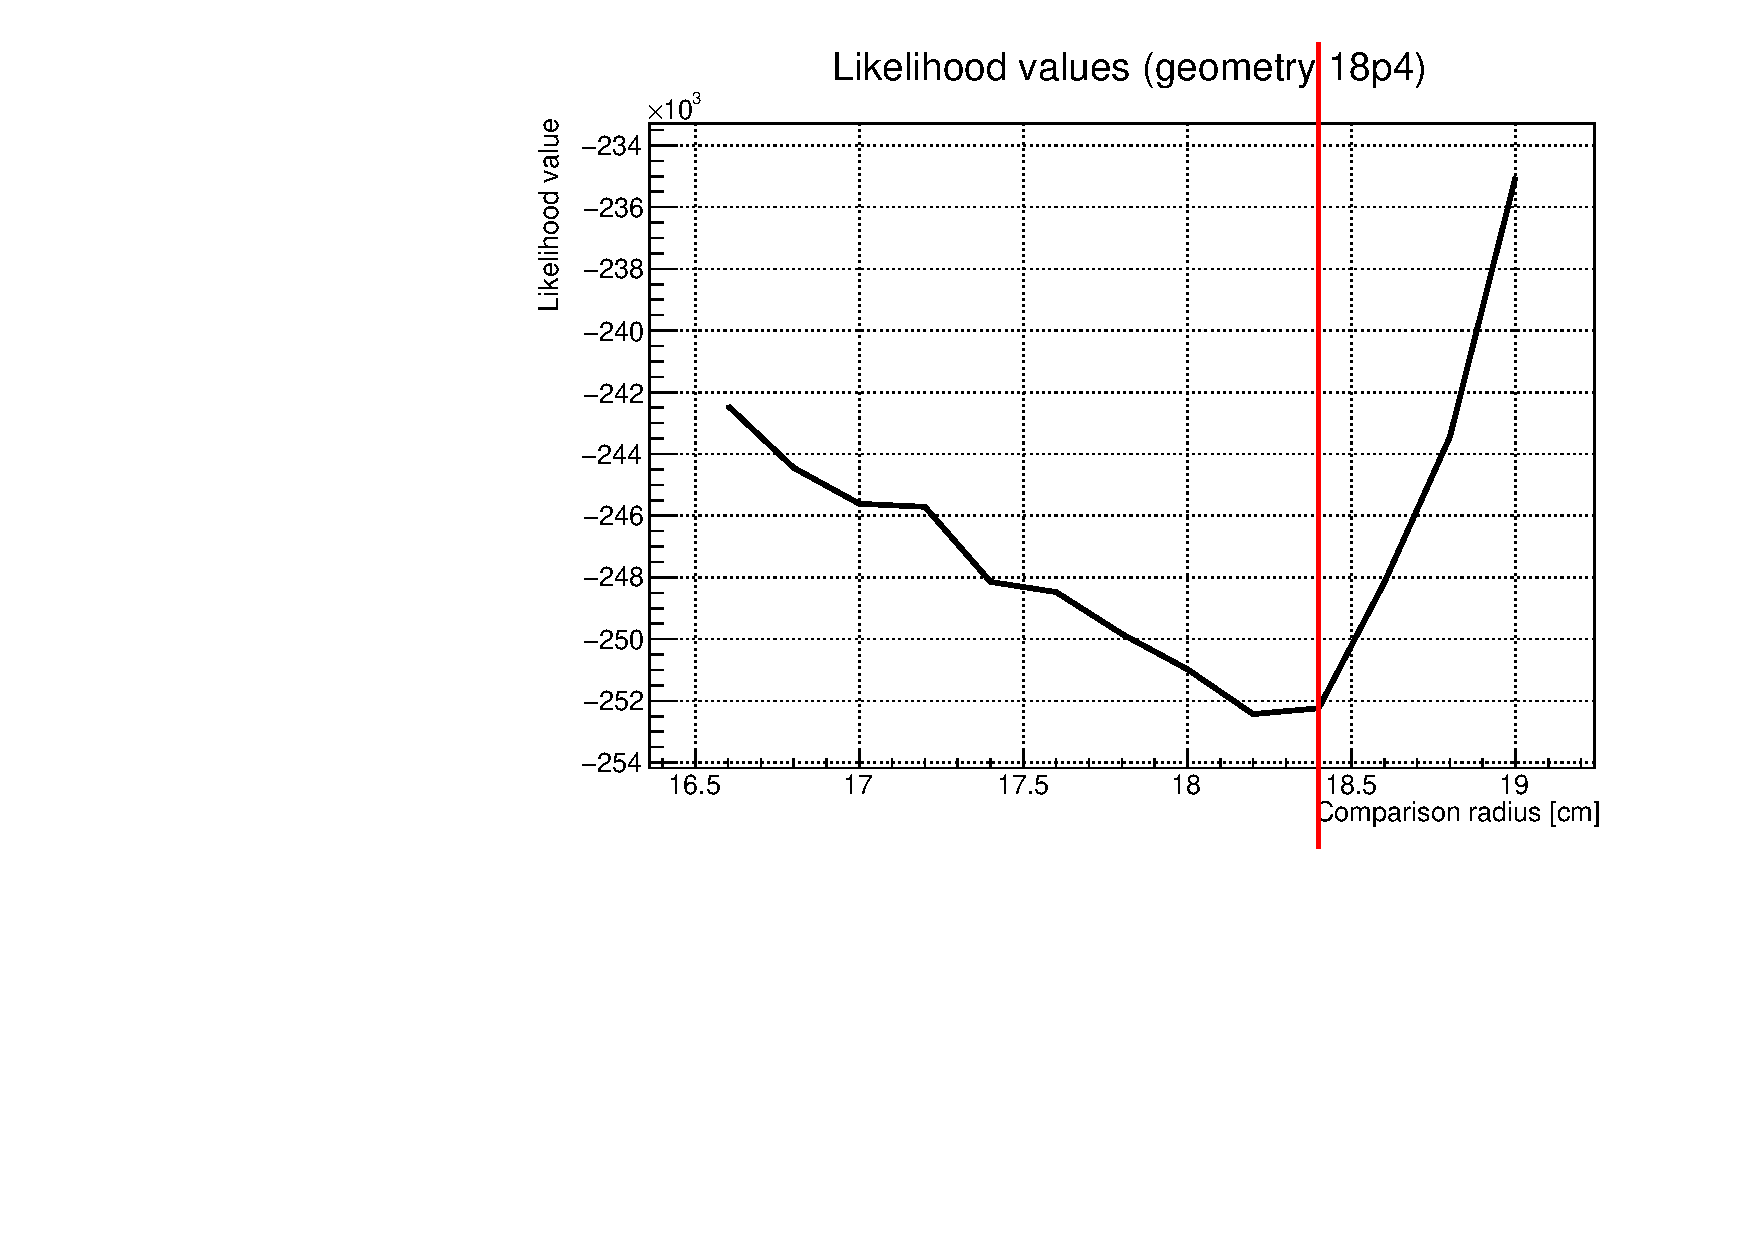
\includegraphics[width=4.2cm, height=3.2cm]{figs/likelihood100LowStat/likelihood18p4.pdf} 
\end{minipage}

\vspace{-5pt}
\begin{minipage}[c]{.32\textwidth}
\begin{exampleblock}{} \begin{center}$r = 18.6$cm\end{center} \end{exampleblock}
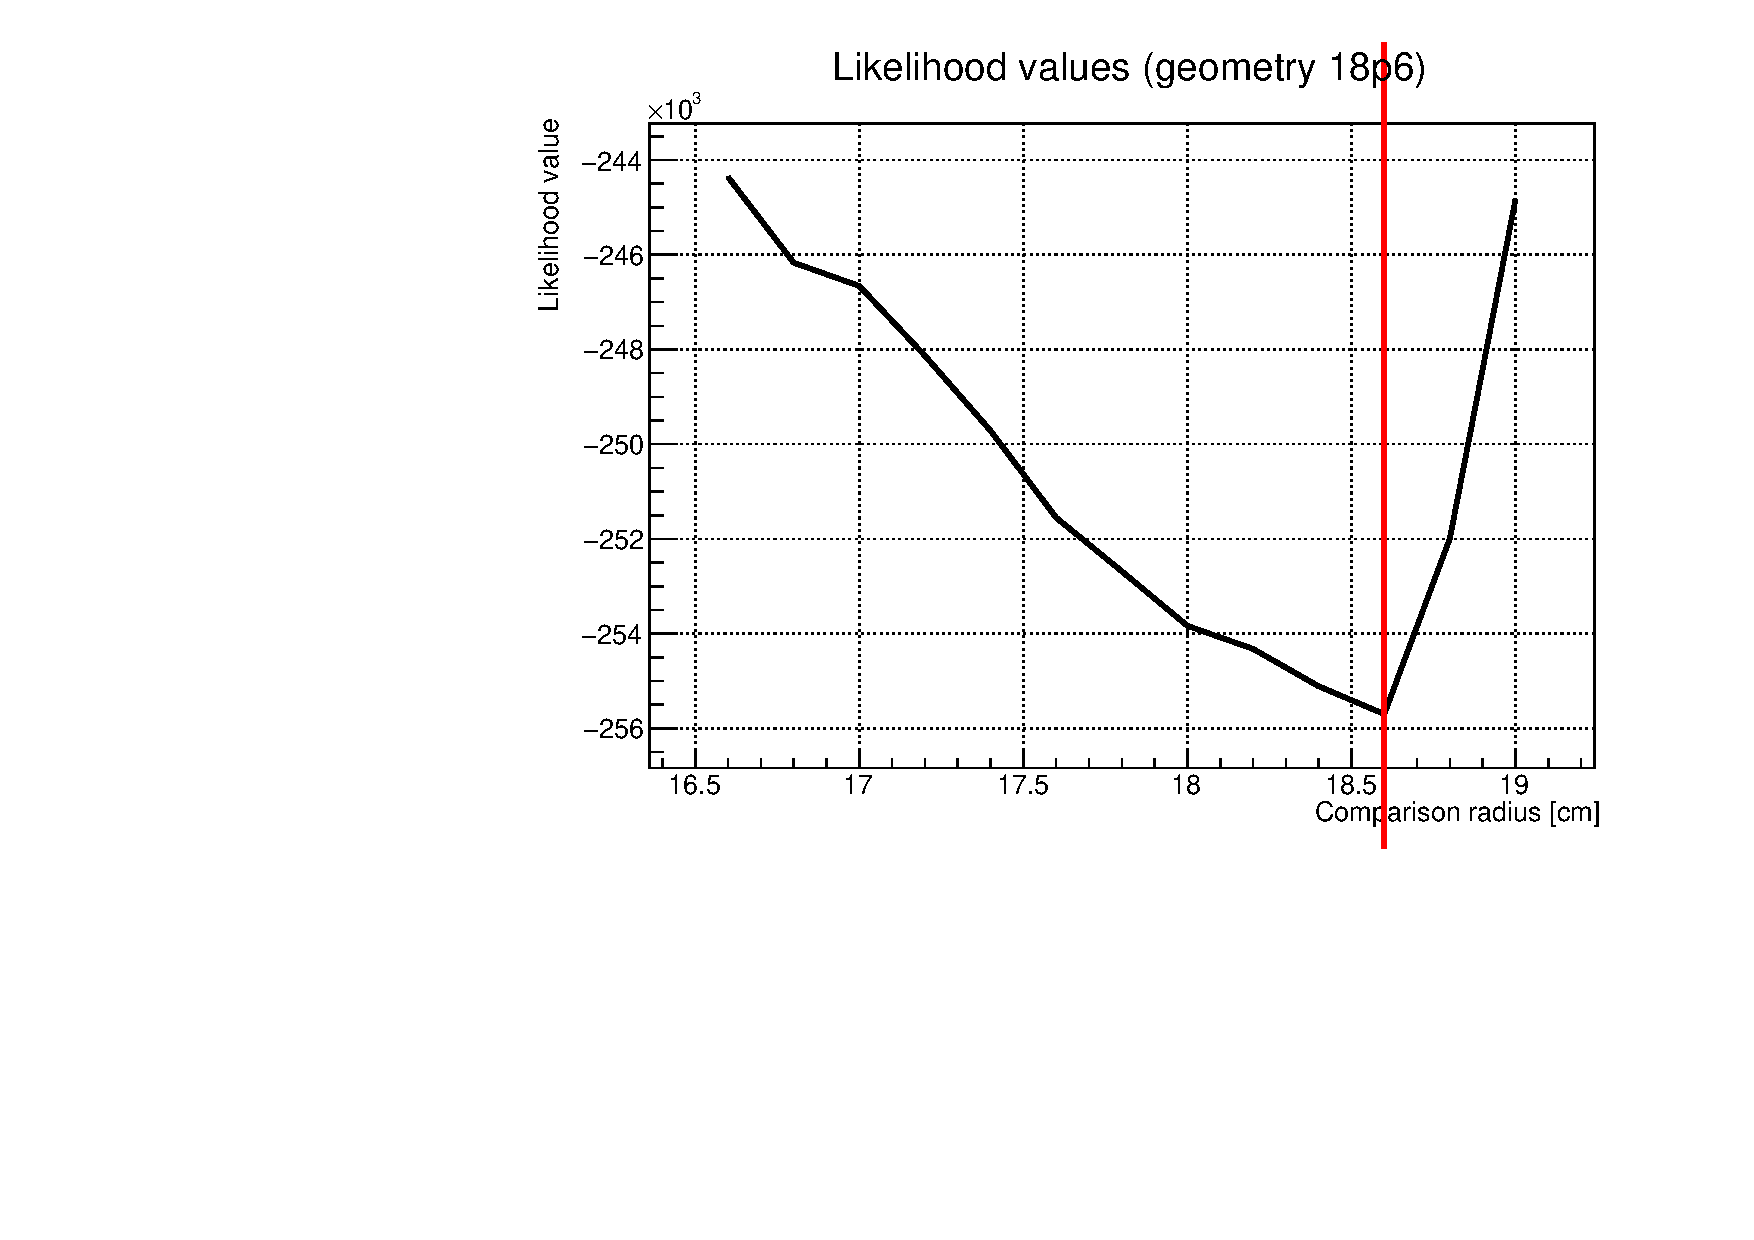
\includegraphics[width=4.2cm, height=3.2cm]{figs/likelihood100LowStat/likelihood18p6.pdf} 
\end{minipage}
\begin{minipage}[c]{.32\textwidth}
\begin{exampleblock}{} \begin{center}$r = 18.8$cm\end{center} \end{exampleblock}
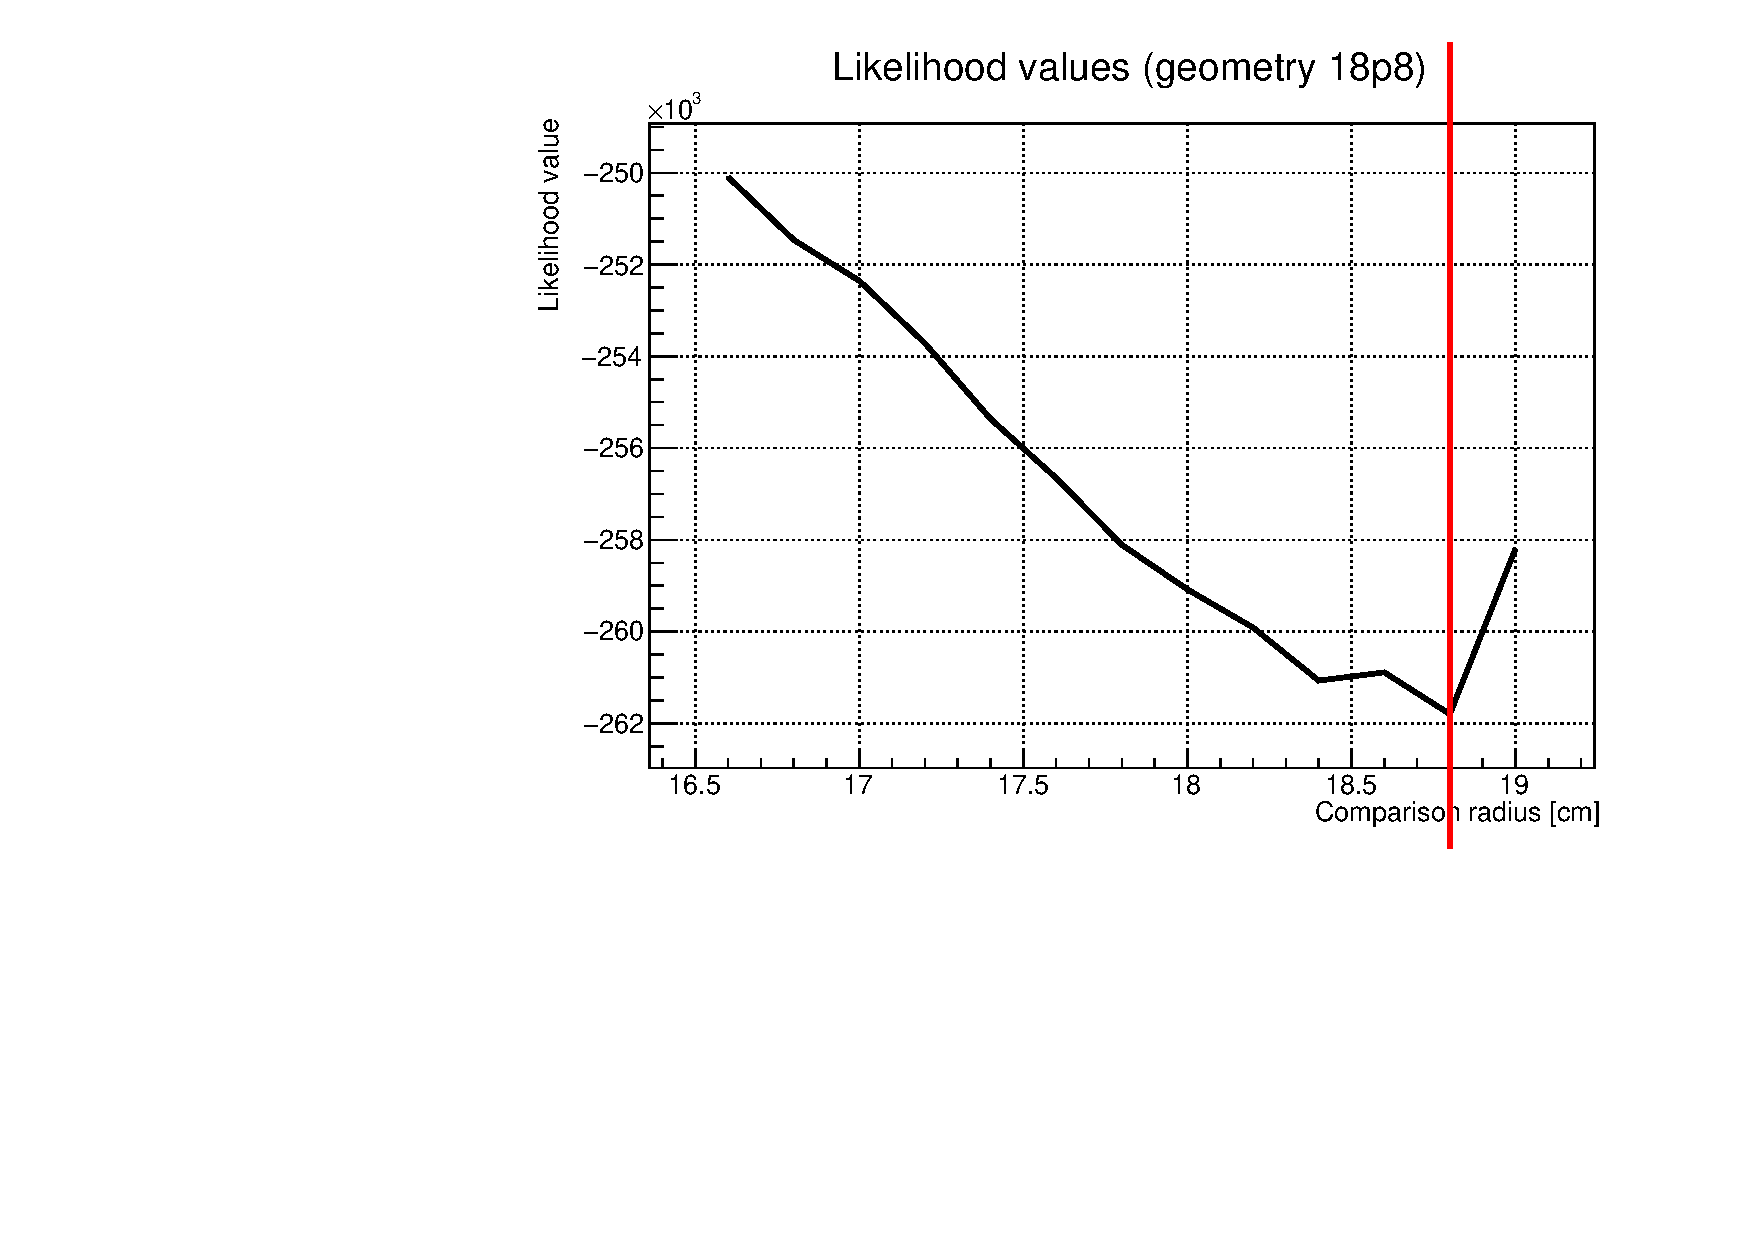
\includegraphics[width=4.2cm, height=3.2cm]{figs/likelihood100LowStat/likelihood18p8.pdf} 
\end{minipage}
\begin{minipage}[c]{.32\textwidth}
\begin{exampleblock}{} \begin{center}$r = 19.0$cm\end{center} \end{exampleblock}
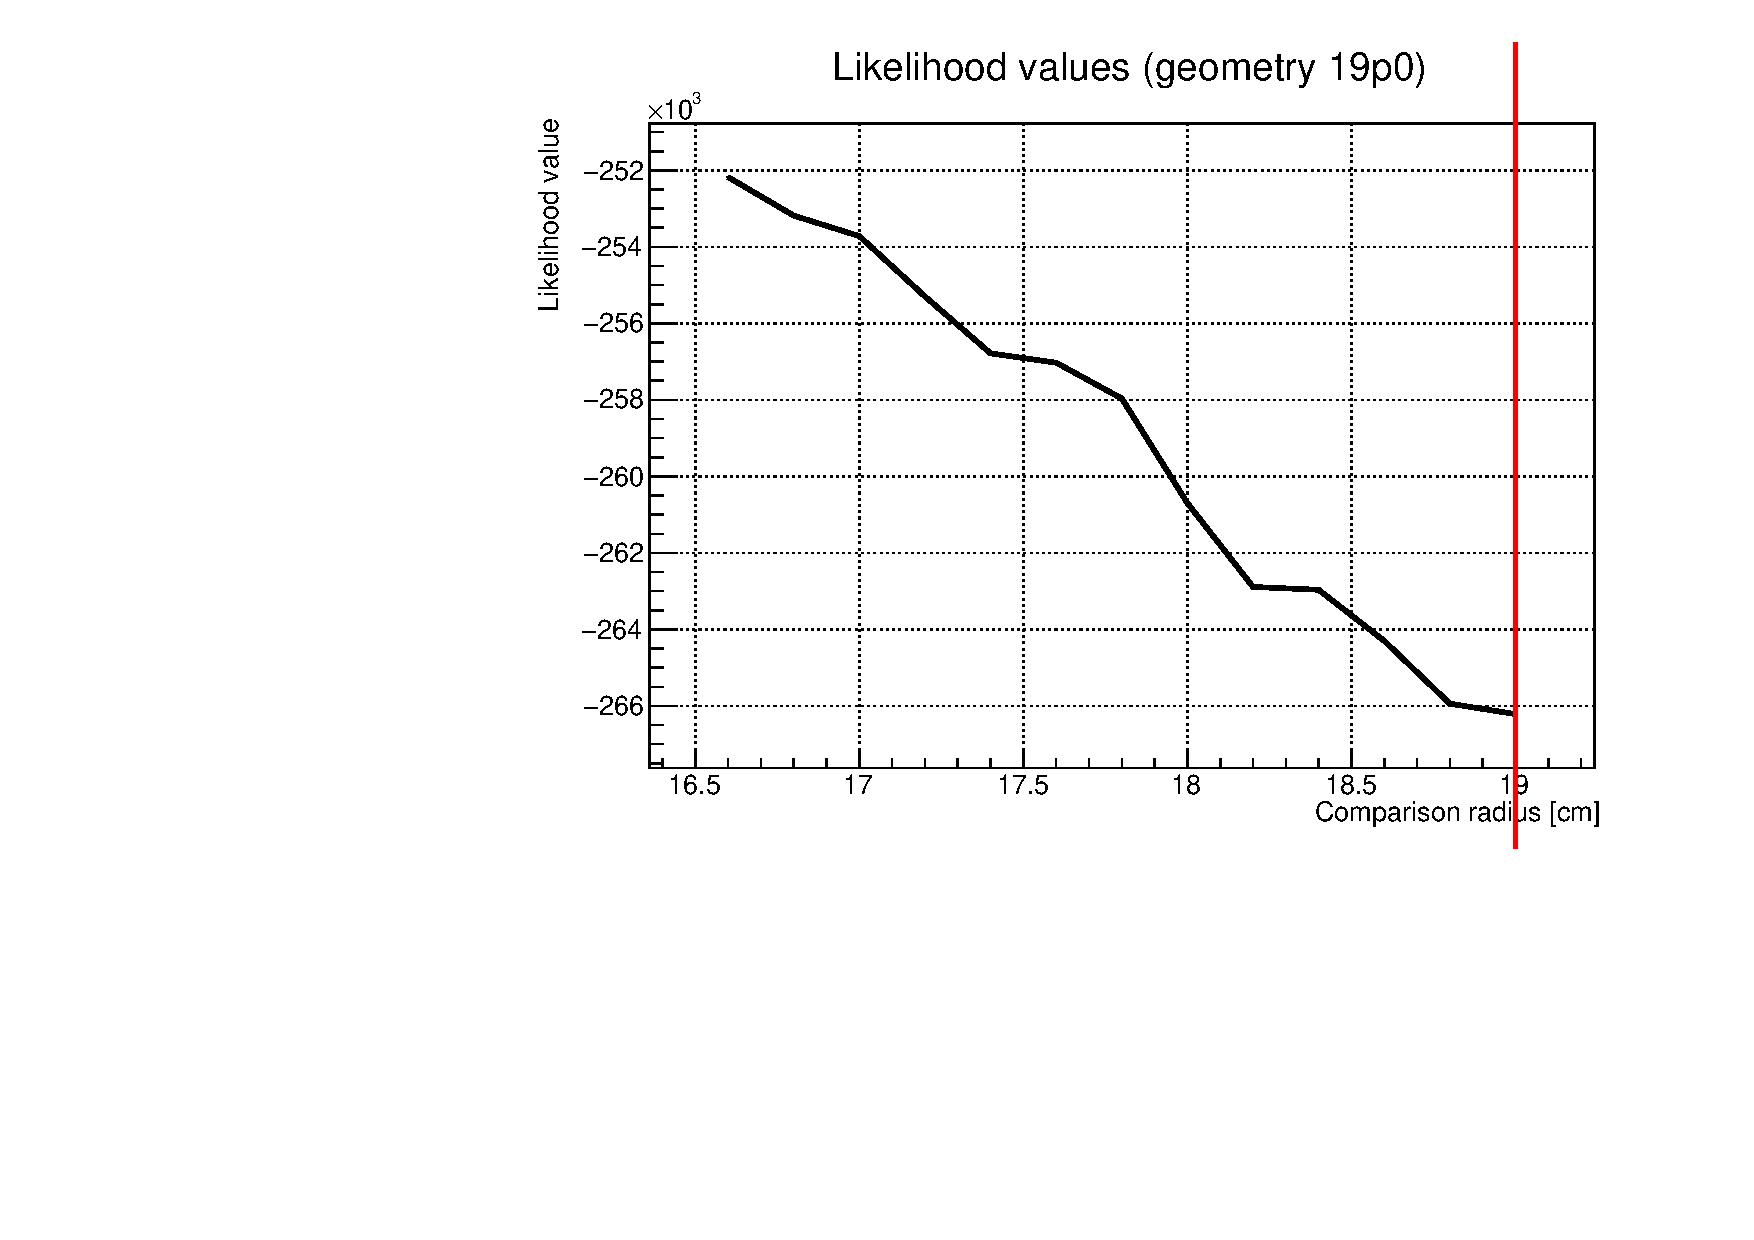
\includegraphics[width=4.2cm, height=3.2cm]{figs/likelihood100LowStat/likelihood19p0.pdf} 
\end{minipage}
\end{frame}

\begin{frame}{Likelihood curves (50.000 events, 100 iterations)}
\justifying
\begin{minipage}[c]{.32\textwidth}
\begin{exampleblock}{} \begin{center}$r = 16.8$cm\end{center} \end{exampleblock}
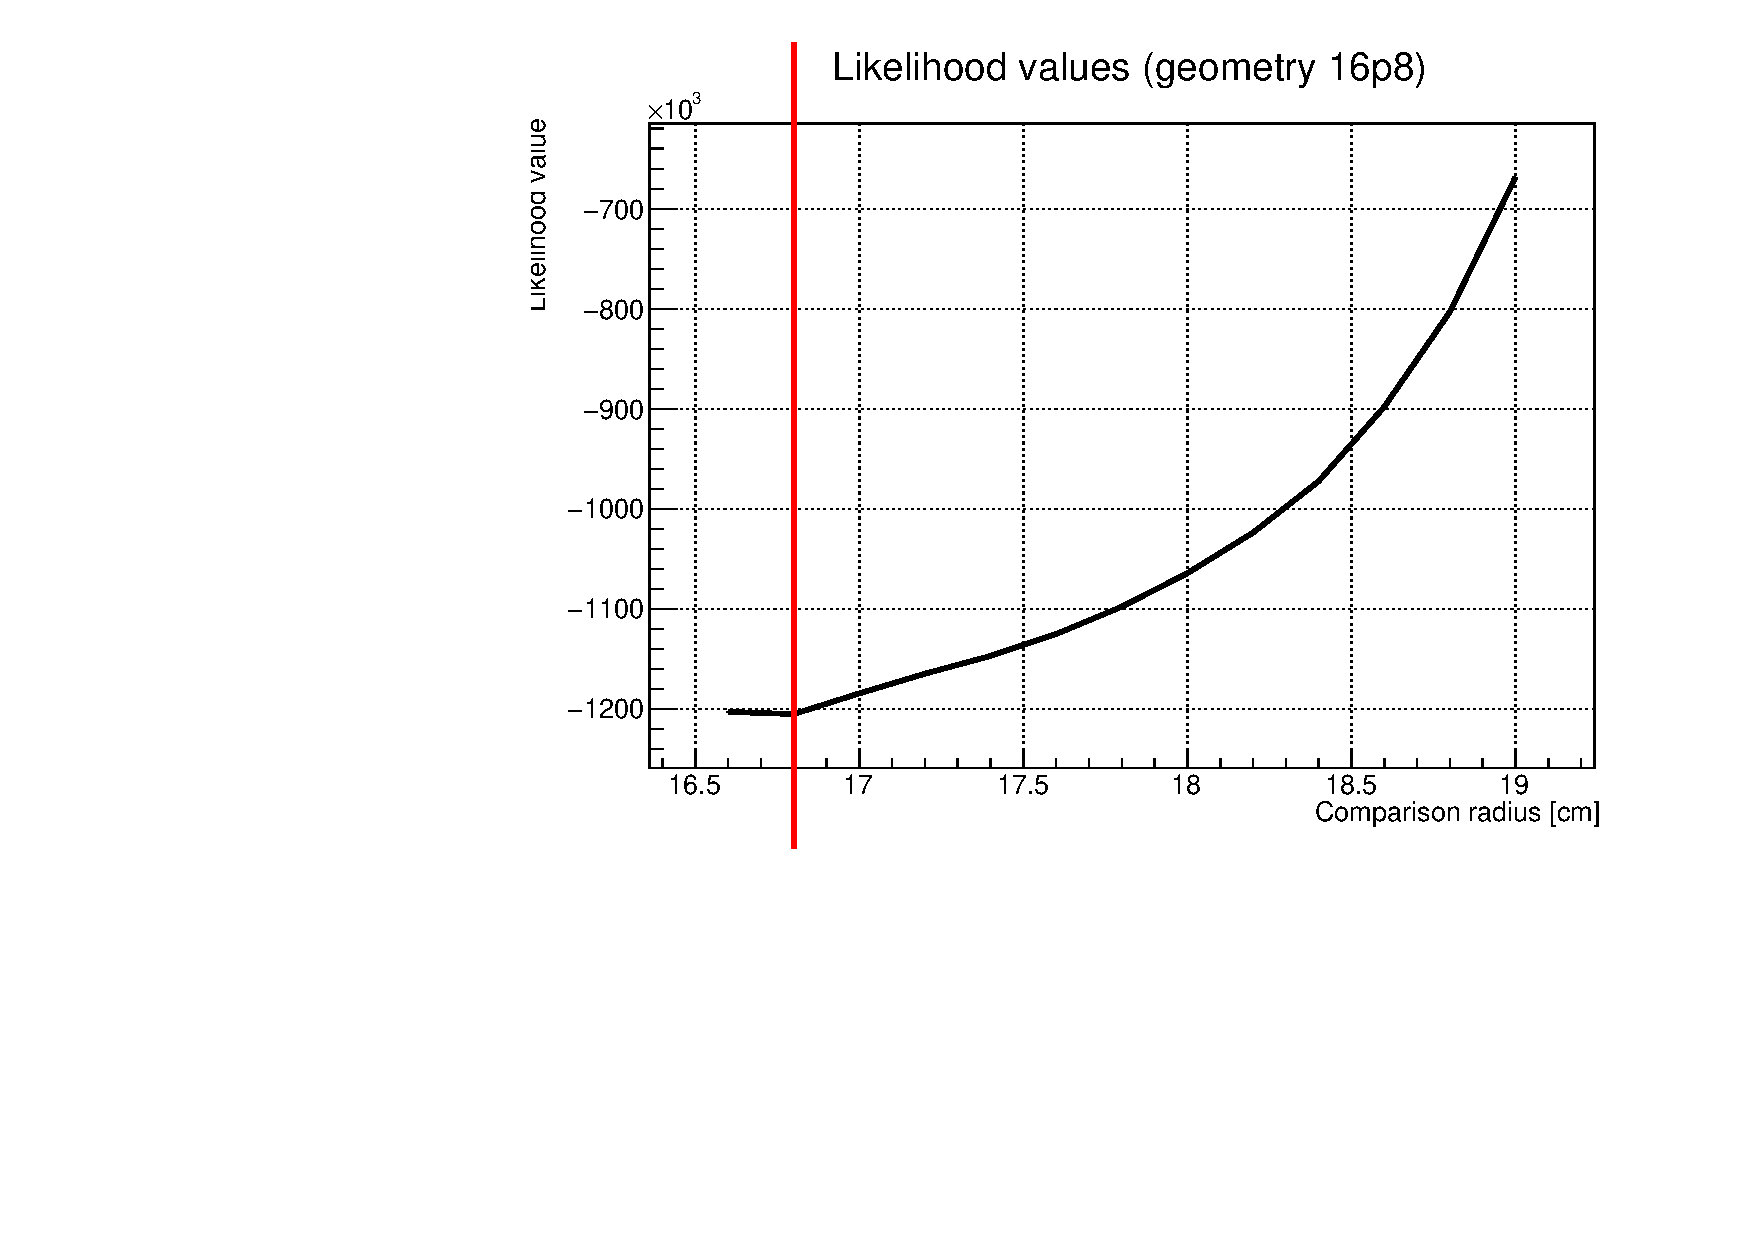
\includegraphics[width=4.2cm, height=3.2cm]{figs/likelihood100HighStat/likelihood16p8.pdf} 
\end{minipage}
\begin{minipage}[c]{.32\textwidth}
\begin{exampleblock}{} \begin{center}$r = 17.0$cm\end{center} \end{exampleblock}
\includegraphics[width=4.2cm, height=3.2cm]{figs/likelihood100HighStat/likelihood17p0.pdf} 
\end{minipage}
\begin{minipage}[c]{.32\textwidth}
\begin{exampleblock}{} \begin{center}$r = 17.2$cm\end{center} \end{exampleblock}
\includegraphics[width=4.2cm, height=3.2cm]{figs/likelihood100HighStat/likelihood17p2.pdf} 
\end{minipage}

\vspace{-5pt}
\begin{minipage}[c]{.32\textwidth}
\begin{exampleblock}{} \begin{center}$r = 17.4$cm\end{center} \end{exampleblock}
\includegraphics[width=4.2cm, height=3.2cm]{figs/likelihood100HighStat/likelihood17p4.pdf} 
\end{minipage}
\begin{minipage}[c]{.32\textwidth}
\begin{exampleblock}{} \begin{center}$r = 17.6$cm\end{center} \end{exampleblock}
\includegraphics[width=4.2cm, height=3.2cm]{figs/likelihood100HighStat/likelihood17p6.pdf} 
\end{minipage}
\begin{minipage}[c]{.32\textwidth}
\begin{exampleblock}{} \begin{center}$r = 17.8$cm\end{center} \end{exampleblock}
\includegraphics[width=4.2cm, height=3.2cm]{figs/likelihood100HighStat/likelihood17p8.pdf} 
\end{minipage}
\end{frame}

\begin{frame}{Likelihood curves (50.000 events, 100 iterations)}
\justifying
\begin{minipage}[c]{.32\textwidth}
\begin{exampleblock}{} \begin{center}$r = 18.0$cm\end{center} \end{exampleblock}
\includegraphics[width=4.2cm, height=3.2cm]{figs/likelihood100HighStat/likelihood18p0.pdf} 
\end{minipage}
\begin{minipage}[c]{.32\textwidth}
\begin{exampleblock}{} \begin{center}$r = 18.2$cm\end{center} \end{exampleblock}
\includegraphics[width=4.2cm, height=3.2cm]{figs/likelihood100HighStat/likelihood18p2.pdf} 
\end{minipage}
\begin{minipage}[c]{.32\textwidth}
\begin{exampleblock}{} \begin{center}$r = 18.4$cm\end{center} \end{exampleblock}
\includegraphics[width=4.2cm, height=3.2cm]{figs/likelihood100HighStat/likelihood18p4.pdf} 
\end{minipage}

\vspace{-5pt}
\begin{minipage}[c]{.32\textwidth}
\begin{exampleblock}{} \begin{center}$r = 18.6$cm\end{center} \end{exampleblock}
\includegraphics[width=4.2cm, height=3.2cm]{figs/likelihood100HighStat/likelihood18p6.pdf} 
\end{minipage}
\begin{minipage}[c]{.32\textwidth}
\begin{exampleblock}{} \begin{center}$r = 18.8$cm\end{center} \end{exampleblock}
\includegraphics[width=4.2cm, height=3.2cm]{figs/likelihood100HighStat/likelihood18p8.pdf} 
\end{minipage}
\begin{minipage}[c]{.32\textwidth}
\begin{exampleblock}{} \begin{center}$r = 19.0$cm\end{center} \end{exampleblock}
\includegraphics[width=4.2cm, height=3.2cm]{figs/likelihood100HighStat/likelihood19p0.pdf} 
\end{minipage}
\end{frame}

\begin{frame}{Likelihood curves (10.000 events, 250 iterations)}
\justifying
\begin{minipage}[c]{.32\textwidth}
\begin{exampleblock}{} \begin{center}$r = 16.8$cm\end{center} \end{exampleblock}
\includegraphics[width=4.2cm, height=3.2cm]{figs/likelihood250LowStat/likelihood16p8.pdf} 
\end{minipage}
\begin{minipage}[c]{.32\textwidth}
\begin{exampleblock}{} \begin{center}$r = 17.0$cm\end{center} \end{exampleblock}
\includegraphics[width=4.2cm, height=3.2cm]{figs/likelihood250LowStat/likelihood17p0.pdf} 
\end{minipage}
\begin{minipage}[c]{.32\textwidth}
\begin{exampleblock}{} \begin{center}$r = 17.2$cm\end{center} \end{exampleblock}
\includegraphics[width=4.2cm, height=3.2cm]{figs/likelihood250LowStat/likelihood17p2.pdf} 
\end{minipage}

\vspace{-5pt}
\begin{minipage}[c]{.32\textwidth}
\begin{exampleblock}{} \begin{center}$r = 17.4$cm\end{center} \end{exampleblock}
\includegraphics[width=4.2cm, height=3.2cm]{figs/likelihood250LowStat/likelihood17p4.pdf} 
\end{minipage}
\begin{minipage}[c]{.32\textwidth}
\begin{exampleblock}{} \begin{center}$r = 17.6$cm\end{center} \end{exampleblock}
\includegraphics[width=4.2cm, height=3.2cm]{figs/likelihood250LowStat/likelihood17p6.pdf} 
\end{minipage}
\begin{minipage}[c]{.32\textwidth}
\begin{exampleblock}{} \begin{center}$r = 17.8$cm\end{center} \end{exampleblock}
\includegraphics[width=4.2cm, height=3.2cm]{figs/likelihood250LowStat/likelihood17p8.pdf} 
\end{minipage}
\end{frame}

\begin{frame}{Likelihood curves (10.000 events, 250 iterations)}
\justifying
\begin{minipage}[c]{.32\textwidth}
\begin{exampleblock}{} \begin{center}$r = 18.0$cm\end{center} \end{exampleblock}
\includegraphics[width=4.2cm, height=3.2cm]{figs/likelihood250LowStat/likelihood18p0.pdf} 
\end{minipage}
\begin{minipage}[c]{.32\textwidth}
\begin{exampleblock}{} \begin{center}$r = 18.2$cm\end{center} \end{exampleblock}
\includegraphics[width=4.2cm, height=3.2cm]{figs/likelihood250LowStat/likelihood18p2.pdf} 
\end{minipage}
\begin{minipage}[c]{.32\textwidth}
\begin{exampleblock}{} \begin{center}$r = 18.4$cm\end{center} \end{exampleblock}
\includegraphics[width=4.2cm, height=3.2cm]{figs/likelihood250LowStat/likelihood18p4.pdf} 
\end{minipage}

\vspace{-5pt}
\begin{minipage}[c]{.32\textwidth}
\begin{exampleblock}{} \begin{center}$r = 18.6$cm\end{center} \end{exampleblock}
\includegraphics[width=4.2cm, height=3.2cm]{figs/likelihood250LowStat/likelihood18p6.pdf} 
\end{minipage}
\begin{minipage}[c]{.32\textwidth}
\begin{exampleblock}{} \begin{center}$r = 18.8$cm\end{center} \end{exampleblock}
\includegraphics[width=4.2cm, height=3.2cm]{figs/likelihood250LowStat/likelihood18p8.pdf} 
\end{minipage}
\begin{minipage}[c]{.32\textwidth}
\begin{exampleblock}{} \begin{center}$r = 19.0$cm\end{center} \end{exampleblock}
\includegraphics[width=4.2cm, height=3.2cm]{figs/likelihood250LowStat/likelihood19p0.pdf} 
\end{minipage}
\end{frame}

\begin{frame}{Future improvements}
\justifying
This exercise is only a first approach to the problem, and different improvements can be considered to \textbf{improve and/or generalize the results obtained}:
\begin{itemize}
\justifying
\item Consider more general geometries that a pipe, or perform the likelihood minimization with respect to additional parameters, not only the thickness of the pipe
\item The analysis can be repeated using actual data collected by the detector
\item We could also consider the ionization process to improve these results
\item The interaction between the detector and the cosmic muons could be considered in our Generator to make it more reliable and precise
\item A further analysis estimating the Hessian of the likelihoods and the impact of systematic uncertainties would definitely improve the algorithm
\item Finally, we have been limited computionally in this case, taking a few hours to produce a single plot with few statistics. Accessing to computers with higher capacities will be extremely interesting to improve the results obtained.
\end{itemize}
\end{frame}

\backupend


 \end{document}